%%%*******************************************************************************
%  Classe Latex UEFS PPGM, Version 1.0.1 13/09/2021
%
%  Define as normas e estilo das dissertações e teses do PPGM-UEFS
%
%  Author : Gilney Zebende
%  Contribuição : João Paulo Just Peixoto <joao.just@ifba.edu.br,just1982@gmail.com>
%%%-------------------------------------------------------------------------------

%%%-------------------------------------------------------------------------------
%  DOCUMENTAÇÃO COM EXEMPLOS
%%%*******************************************************************************

%%%-------------------------------------------------------------------------------
%%% Thesis default options
%%%-------------------------------------------------------------------------------
%\documentclass[subook]{Classes/PPGM-UEFS}
%\documentclass[sureport]{Classes/PPGM-UEFS}

%%%-------------------------------------------------------------------------------
%%% Thesis custom options
%%%-------------------------------------------------------------------------------

%%% Fancy page headings
%\documentclass[fancyheadings, subook]{Classes/PPGM-UEFS}
%\documentclass[fancyheadings, sureport]{Classes/PPGM-UEFS}

%%% Fancy chapters and sections headings
%\documentclass[fancychapter, subook]{Classes/PPGM-UEFS}
%\documentclass[fancychapter, sureport]{Classes/PPGM-UEFS}

%%% Fancy page , chapters and sections headings
%\documentclass[fancyheadings, fancychapter, subook]{Classes/PPGM-UEFS}
\documentclass[fancyheadings, fancychapter, sureport]{PPGM-UEFS}


%%%-------------------------------------------------------------------------------
%%% Thesis Commands (ONLY with fancy page headings)
%%%-------------------------------------------------------------------------------

%%%Page header line width
%\footlinewidth{value}

%%%Page footer line width
%\headlinewidth{value}

%%%Page header and footer line width
%\headingslinewidth{value}

%%%Page header and footer lines without text
%\headingslinesonly

%%%The default line width is 0.3pt.
%%%Set the value to 0pt to remove the page header and/or footer line

%%%-------------------------------------------------------------------------------
%%% SUThesis Supported Graphic Formats
%%%-------------------------------------------------------------------------------
% The figures formats supported depend upon the selected output file
% Include your figure without the extention, the SUThesis will automatically
% search the predefined `Figures' directory tree for the right file format.
%
% - The pdfLaTEX (PDF) supports graphics inclusions in PDF, JPG, PNG, and
%   MetaPost (with .mps extention) formats.
%
% - The Latex (DVI) supports graphics inclusions in EPS and PS formats.
%%%-------------------------------------------------------------------------------


%%%-------------------------------------------------------------------------------
%%% Árvore de diretório PPGM-UEFS
%%%-------------------------------------------------------------------------------
%  Diretorio
%       \Classes        (requerido)
%       \Figures        (requerido) --------------------------------->
%       \Figures\PDF    (opcional)
%       \Figures\JPG    (opcional) Figuras nestas pastas
%       \Figures\PNG    (opcional) são buscadas automaticamente
%       \Figures\MPS    (opcional) pela classe PPGM-UEFS.
%       \Figures\EPS    (opcional)
%       \Figures\PS     (opcional) <--------------------------------
%       \Tables         (requerido)
%       \Others         (requerido)
%       \Chapters       (requerido)
%       \Appendices     (opcional)
%       \References     (requerido)
%%%-------------------------------------------------------------------------------

%%%-------------------------------------------------------------------------------
%%% Funções auxiliares (não mude isso)
%%%-------------------------------------------------------------------------------
\newcommand{\nth}[2]{
    \foreach \x [count=\k] in #1 {
        \ifnum\k=#2
            \x
        \fi
    }
}

\makeatletter
\newcommand*\ppgmbancalist{}
\newcommand*\ppgmbancaextlist{}
\newcommand*\ppgmbanca[2]{
    \g@addto@macro\ppgmbancalist{{#1,#2},}
}
\newcommand*\ppgmbancaext[2]{
    \g@addto@macro\ppgmbancaextlist{{#1,#2},}
}
\makeatother

%%%-------------------------------------------------------------------------------
%%% Dados da tese/dissertação
%%%-------------------------------------------------------------------------------
\newif\ifdoutor
\newif\ifcoor

%% Primeiro indique se é uma tese de doutorado ou dissertação de mestrado:
\doutortrue     % Para tese de doutorado
%\doutorfalse   % Para dissertação de mestrado

%% Indique também se tem co-orientador
\coortrue       % Tenho co-orientador
%\coorfalse     % Não tenho co-orientador

%% Preencha as informações abaixo
\newcommand{\ppgmtitulo}       {Gerenciamento de crise nas cidades através de tecnologias de sensoriamento e modelagem de emergências}
\newcommand{\ppgmsubtitulo}    {Sub-título da Dissertação ou Tese}
\newcommand{\ppgmautor}        {João Paulo Just Peixoto}
\newcommand{\ppgmorientador}   {Daniel G. Costa}
\newcommand{\ppgmcoorientador} {Washington de J. S. da Franca Rocha}
\newcommand{\ppgmcooruniv}     {UNIVERSIDADE ESTADUAL DE FEIRA DE SANTANA} % Instituição do co-orientador
\newcommand{\ppgmpalavraschave}{cidades inteligentes, gerenciamento de crises, modelos urbanos, redes de sensores, internet das coisas}
\newcommand{\ppgmkeywords}     {smart cities, crisis management, urban models, sensor networks, internet of things}
\newcommand{\ppgmdia}          {28}
\newcommand{\ppgmmes}          {maio}
\newcommand{\ppgmano}          {2023}
\newcommand{\ppgmcidade}       {Feira de Santana, BA}

%% Indique os membros internos da banca (nome e instituição)
% É possível acrescentar membros copiando o comando
%\ppgmbanca{Prof. Dr. Washington de J. S. da Franca Rocha}{\ppgmcooruniv}
\ppgmbanca{Profa. Dra. Rosângela Leal Santos}{\ppgmcooruniv}

%% Indique os membros externos da banca (nome e instituição)
\ppgmbancaext{Prof. Dr. Thiago C. Jesus}{UNIVERSIDADE ESTADUAL DE FEIRA DE SANTANA}
\ppgmbancaext{Prof. Dr. Eduardo Cambruzzi}{INSTITUTO FEDERAL DA BAHIA}


%%%-------------------------------------------------------------------------------
%%% Sumário do PDF
%%%-------------------------------------------------------------------------------
\ifdoutor
    \newcommand{\ppgmsubject}{Tese de Doutorado em Modelagem em Ciências da Terra e do Ambiente}
\else
    \newcommand{\ppgmsubject}{Dissertação de Mestrado em Modelagem em Ciências da Terra e do Ambiente}
\fi

\ifpdf
    \hypersetup{
                colorlinks  = true,
                pdftitle    = \ppgmtitulo,
                pdfauthor   = \ppgmautor,
                pdfsubject  = \ppgmsubject,
                pdfcreator  = PPGM-UEFS,
                pdfproducer = PDFLatex,
                pdfkeywords = \ppgmpalavraschave
    }
\fi

%%%-------------------------------------------------------------------------------
%%% Required packages
%%%-------------------------------------------------------------------------------
% - ifthen
% - setspace
% - amsmath
% - amsfonts
% - amssymb
% - amsthm
% - eucal
% - graphics
% - fancyhdr
%%%-------------------------------------------------------------------------------

%%%-------------------------------------------------------------------------------
%%% Optional packages
%%%-------------------------------------------------------------------------------
%\usepackage[latin1]{inputenc}
\usepackage[utf8]{inputenc}
\usepackage{longtable}
\usepackage{multirow}
\usepackage{lscape}
\usepackage{graphicx}
\usepackage{float,subfigure}
\usepackage{makecell}
\usepackage{tikz}
\usepackage{algorithm}
\usepackage{algorithmic}
\usepackage{listings}
\usepackage{lipsum}
\usepackage{caption}

% Múltiplas referências
\usepackage[backend=biber,style=abnt,giveninits,repeatfields,extrayear]{biblatex}
\addbibresource{Chapters/1-Survey/references.bib}
\addbibresource{Chapters/2-EDUs/references.bib}
\addbibresource{Chapters/3-CityZones/references.bib}

\usepackage[left=3cm,top=3cm,right=2cm,bottom=2cm]{geometry}
\usepackage{ifpdf}
% Tables and Figures Caption
\setlength{\LTcapwidth}{\textwidth}

%\newtheorem{theorem}{Teorema}
%\newtheorem{definition}[theorem]{Defini\c{c}\~ao}

\usepackage{hyperref}

% Traduz os títulos dos algoritmos
\makeatletter
\renewcommand{\ALG@name}{Algoritmo}
\renewcommand{\listalgorithmname}{Lista de  \ALG@name s}
\renewcommand{\algorithmicrequire}{\textbf{Entrada:}}
\renewcommand{\algorithmicensure}{\textbf{Saída:}}
\makeatother

%%%-------------------------------------------------------------------------------
%%% Documento raiz da tese/dissertação
%%%-------------------------------------------------------------------------------
\begin{document}
    %%----------------------------------------------------------------------------
    %% Página de título
    %%----------------------------------------------------------------------------
    % Informações da capa. Não é preciso mudar nada aqui.
    \university{UNIVERSIDADE ESTADUAL DE FEIRA DE SANTANA}
    \faculty{Programa de Pós-graduação em Modelagem em Ciências da Terra e do Ambiente}
    
    \ifdoutor
        \course{Doutorado em Modelagem em Ciências da Terra e do Ambiente}
        \typework{Tese de doutorado}
        \thesisdegreetitle{Doutor em Modelagem em Ciências Ambientais}
    \else
        \course{Mestrado em Modelagem em Ciências da Terra e do Ambiente}
        \typework{Dissertação de Mestrado}
        \thesisdegreetitle{Mestre em Ciências Ambientais}
    \fi
    
    \thesistitle{\ppgmtitulo}
    \hidevolume
    \thesisvolume{Volume 1 de 1}
    \thesisauthor{\ppgmautor}
    \thesisadvisor{\ppgmorientador}
    \ifcoor
        % Caso não queira exibir o nome do(a) co-orientador(a), habilite a linha abaixo:
        %\hidecoadvisor 
        \thesiscoadvisor{\ppgmcoorientador}
    \fi
    \thesismonthyear{\ppgmmes\space de \ppgmano}
    \maketitlepage

    %%----------------------------------------------------------------------------
    %% Inserir Folha de rosto, Nota de estilo, folha de assinaturas, dedicatória
    %%----------------------------------------------------------------------------
    % Comente qualquer linha que não queira inserir
    %==========================================================
%        Document: PPGM-UEFS
%        File....: FolhaRosto.TEX
%        Author..: Gilney Zebende, João Paulo Just Peixoto
%        Date....: 13 de setembro de 2021
%==========================================================
\begin{folharosto}

\begin{center}
\theauthor
\end{center}
\ \\
\ \\
\ \\
\ \\
\ \\
\begin{spacing}{2}
   \begin{center}
   {\LARGE {\bf \thetitle}}
   \end{center}
\end{spacing}
\ \\
\ \\
\ \\
\begin{flushright}

   \begin{list}{}{
      \setlength{\leftmargin}{4.5cm}
      \setlength{\rightmargin}{0cm}
      \setlength{\labelwidth}{0pt}
      \setlength{\labelsep}{\leftmargin}}

      \item \thetypework apresentada ao \thefaculty, Curso de \thecourse
      da \theuniversity, como requisito parcial para a obtenção do
      título de {\bf \thedegreetitle}.

    \begin{list}{}{
      \setlength{\leftmargin}{0cm}
      \setlength{\rightmargin}{0cm}
      \setlength{\labelwidth}{0pt}
      \setlength{\labelsep}{\leftmargin}}

      \item Área de conhecimento: Estudos Ambientais e Geotecnologias

      \item Orientador: Dr. \theadvisor
      \newline \hspace*{2.1cm}  {\footnotesize {\it \theuniversity}}
      
      \ifcoor
          \item Co-orientador: Dr. \thecoadvisor
          \newline \hspace*{2.1cm}  {\footnotesize \emph{\ppgmcooruniv}}
      \fi
      \end{list}
   \end{list}

\end{flushright}

\vspace*{\fill}

%\begin{spacing}{1.5}
   \begin{center}
   \ppgmcidade \par
   \theuniversity \par
   \ppgmano
   \end{center}
%\end{spacing}

\end{folharosto}

    %==========================================================
%        Document: PPGM-UEFS
%        File....: NotaEstilo.TEX
%        Author..: Gilney Zebende
%        Date....: 24 de abril de 2018
%==========================================================

\begin{notaestilo}
Esta \thetypeworkthree foi elaborada considerando as normas de estilo propostas e aprovadas pelo colegiado do \thefacultytwo e est\~ao dispon\'iveis no formato eletr\^onico (\url{http://ppgm.uefs.br/banco-de-dissertacoes}) ou no formato impresso para consulta. \\


\end{notaestilo}

    %==========================================================
%        Document: PPGM-UEFS
%        File....: FolhaAssinaturas.TEX
%        Author..: Gilney Zebende, João Paulo Just Peixoto
%        Date....: 14 de setembro de 2021
%==========================================================

\begin{folhaassinaturas}

%\thispagestyle{empty}

\def\signature#1#2{\parbox[b]{1in}{\smash{#1}\vskip12pt}
\hfill \parbox[t]{4in}{\shortstack{\vrule width 4in height
0.4pt\\\small#2}}}

\def\InstituicaoMembro#1#2{\parbox[b]{1in}{\smash{#1}\vskip12pt}
\hfill \parbox[t]{4in}{\shortstack{\vrule width 4in \\\small#2}}}

\def\signaturepage{%

    \begin{spacing}{1.5}
        \begin{center}
        {\LARGE \theuniversity} \\
        {\large \thefaculty} \\
        {\large \thecourse} \\
        \end{center}
    \end{spacing}

   \vskip 0.25in plus 0.4in minus 0.1in

    \begin{spacing}{1.0}
        \begin{sloppypar}
        A Banca Examinadora, constitu\'ida pelos professores listados abaixo, leu e recomenda a aprova\c{c}\~ao da
        \thetypeworktwo, intitulada ``\thetitle'',
        apresentada no dia \ppgmdia\space de \ppgmmes\space de \ppgmano, como requisito
        parcial para a obten\c{c}\~ao do t\'itulo de {\bf \thedegreetitle}.\\
        \end{sloppypar}
    \end{spacing}

    \def\sigskip{\vskip0.15in plus 0.2in minus 0.1in}
    \def\beginskip{\vskip0.3875in plus 0.2in minus 0.1in}

    \beginskip
    \signature{Orientador:}{Prof. Dr. \theadvisor} \\
    \InstituicaoMembro{}{\theuniversity} \\

    \ifcoor
        \sigskip
        \beginskip
        \signature{Co-Orientador:}{Prof. Dr. \thecoadvisor} \\
        \InstituicaoMembro{}{\ppgmcooruniv} \\
    \fi

    \foreach \i in \ppgmbancaextlist {
        \ifx\i\empty{}
        \else
            \sigskip
            \beginskip
            \signature{Membro externo da Banca:}{\nth{\i}{1}} \\
            \InstituicaoMembro{}{\nth{\i}{2}} \\
        \fi
    }
    
    \foreach \i in \ppgmbancalist {
        \ifx\i\empty{}
        \else
            \sigskip
            \beginskip
            \signature{Membro interno da Banca:}{\nth{\i}{1}} \\
            \InstituicaoMembro{}{\nth{\i}{2}} \\
        \fi
    }

    \vfill
    \newpage
    \setcounter{page}{3}
}
%*********************************************************************


\signaturepage


\end{folhaassinaturas}

    %==========================================================
%        Document: PPGM-UEFS
%        File....: Dedicatoria.TEX
%        Author..: Gilney Zebende, João Paulo Just Peixoto
%        Date....: 14 de setembro de 2021
%==========================================================

\begin{dedicatoria}
%\thispagestyle{empty}

\vspace*{\fill}

\begin{flushright}
Dedico este trabalho a...
\end{flushright}
\end{dedicatoria}

    %==========================================================
%        Document: PPGM-UEFS
%        File....: Agradecimentos.TEX
%        Author..: Gilney Zebende
%        Date....: 24 de abril de 2018
%==========================================================
% Neste arquivo de agradecimentos é preciso usar \\ para saltar parágrafos.

\begin{agradecimentos}

Agradeço ao Prof. Dr. Daniel G. Costa por ter sido um excelente orientador, desde a época do mestrado. Foi a partir das suas valiosas orientações, ensinamentos e conselhos que pude crescer como pesquisador e adquirir a prática da escrita de artigos. Agradeço também por suas ideias e sugestões, desde temas de artigos ao projeto do doutorado. Além disso, com sua ajuda pude alcançar um dos meus sonhos como acadêmico que era estudar por uma temporada no exterior, que foi possível através do período de doutorado sanduíche na FEUP. Muito obrigado.

Por falar em FEUP, agradeço também aos professores Dr. Paulo Portugal, que me recebeu para o doutorado sanduíche, e Dr. Francisco Vasques, que além de participar conosco nas pesquisas conseguiu viabilizar minha hospedagem na cidade do Porto.

Agradeço à minha família, minha esposa Alice e meu filho Gustavo, que aturaram meus momentos de concentração total, nos quais eu não podia me dedicar muito a eles como esperado e também por serem minha motivação de crescimento constante. Sem eles eu não teria tanto gás pra trabalhar.

Por fim, agradeço a todos do PPGM pelo excelente trabalho neste programa de pós-graduação. Através das aulas do doutorado pude melhorar ainda mais minha prática de pesquisa, além de conhecer novas ferramentas que acabaram sendo de grande valia durante minha pesquisa.

\noindent
\ppgmcidade, Brasil \hfill \theauthor\\
\ppgmdia\space de \ppgmmes\space de \ppgmano
\end{agradecimentos}


    %%----------------------------------------------------------------------------
    %% Resumo/abstract, sumário e siglas
    %%----------------------------------------------------------------------------
    % Comente qualquer linha que não queira inserir
    \begin{romanpagenumbers}
        % Resumo e abstract
        \begin{thesisresumo}

O crescimento dos grandes centros urbanos tem trazido novos desafios para o planejamento das cidades. O aumento demográfico, o alto tráfego de veículos, as constantes construções, o crescente número de centros comerciais, dentre outros fatores, trazem consigo o aumento do risco no dia a dia dos cidadãos. Emergências e crises podem ocorrer e, devido a essa grande concentração de pessoas e veículos, o resgate e a mitigação tornam-se novos desafios no mundo moderno. Esses desafios exigem o uso das tecnologias e aplicações de cidades inteligentes como soluções para o gerenciamento de crises em grandes centros urbanos. Diante deste problema, esta pesquisa de doutorado tem como objetivo estudar e desenvolver algoritmos, modelos e soluções para o gerenciamento de crises em cidades inteligentes, compreendendo as etapas de detecção, alerta e mitigação, de maneira a produzir uma metodologia generalista para os variados tipos de emergências possíveis em um centro urbano, contribuindo para alcançar as metas dos Objetivos de Desenvolvimento Sustentável da Agenda 2030 da Organização das Nações Unidas.\\

\textbf{Palavras Chaves:} \ppgmpalavraschave

\end{thesisresumo}

        \begin{thesisabastract}

The growth of big urban centers have brought new challenges in cities planning. The demographic growth, the high vehicles traffic, the constant new buildings, the rise of the number of commercial centers, among other factors, increase the risk in citizens daily living. Emergencies and crisis may happen and, because of the great concentration of people and vehicles, rescuing and mitigation become new challenges in the modern world. These challenges demand the use of smart cities technologies and applications as solutions for crisis management in big urban centers. In front of this problem, this doctorate research aims to study and develop algorithms, models and solutions for crisis management in smart cities, comprising detection, alerting and mitigation steps, in a way to produce a generalist mothodology for the various types of emergencies in an urban center, contributing to tackle the goals of Agenda 2030 Sustainable Development Goals of United Nation Organization.\\

\textbf{Keywords:} \ppgmkeywords

\end{thesisabastract}

        
        % Sumários
        \thesiscontents
        
        % Lista de quadros (remova se seu texto não possuir quadros)
        \listofquadro
        
        % Lista de algoritmos (remova se seu texto não possuir algoritmos)
        \listofalgorithms
        
        % Abreviações
        \begin{thesisabbreviations}
\begin{footnotesize}
\begin{longtable}[l]{p{2cm}l}

    %%% Lista de siglas e abreviações
    % Faça conforme o modelo:
    %
    % SIGLA \dotfill & Descrição da sigla \\
    AoI     \dotfill & Area of Interest \\
    AoM     \dotfill & Area of Mitigation \\
    % CAD     \dotfill & Computer-aided Design \\
    CSV     \dotfill & Comma Separated Values \\
    EDU     \dotfill & Event Detection Unit \\
    FCT     \dotfill & \textit{Fundação para a Ciência e a Tecnologia} (Foundation for Science and Technology) \\
    FEUP    \dotfill & \textit{Faculdade de Engenharia da Universidade do Porto} (Faculty of Engineering of University of Porto) \\
    FIFO    \dotfill & First In, First Out \\
    GIS     \dotfill & Geographic Information System \\
    IEEE    \dotfill & Institute of Electrical and Electronics Engineers \\
    IoT     \dotfill & Internet of Things \\
    JSON    \dotfill & JavaScript Object Notation \\
    % LABOTEC \dotfill & Laboratório de Tecnologia \\
    % LARA    \dotfill & Laboratório de Aplicações em Redes Avançado \\
    ML      \dotfill & Mitigation Level \\
    MZ      \dotfill & Mitigation Zone \\
    SDG     \dotfill & Sustainable Development Goals \\
    PoI     \dotfill & Point of Interest \\
    UEFS    \dotfill & \textit{Universidade Estadual de Feira de Santana} (State University of Feira de Santana) \\
    VANET   \dotfill & Vehicular Network \\
    WSN     \dotfill & Wireless Sensors Network \\

\end{longtable}
\end{footnotesize}
\end{thesisabbreviations}


        % Volta à numeração de página padrão
    \end{romanpagenumbers}

    %%----------------------------------------------------------------------------
    %% Inclui capítulos da tese/dissertação
    %%----------------------------------------------------------------------------
    \parskip=\baselineskip
    % Comente qualquer linha que não queira inserir
    % \include{Chapters/Capitulo01}
    % \include{Chapters/Capitulo02}
    % \include{Chapters/Capitulo03}
    % \include{Chapters/Capitulo04}
    % \include{Chapters/Capitulo05}
    % \include{Chapters/Capitulo06}
    % Caso precise de mais capítulos, basta criar novos arquivos e acrescentá-los
    % aqui seguindo o modelo acima
    \selectlanguage{english}
    %\begin{abstract}
%The rapid urbanization process in the last century has deeply changed the way we live and interact with each other. As most people now live in urban areas, cities are experiencing growing demands for more efficient and sustainable public services that may improve the perceived quality of life, specially with the anticipated impacts of climatic changes. In this already complex scenario with increasingly overcrowded urban areas, different types of emergency situations may happen anywhere and anytime, with unpredictable costs in human lives and economic losses. In order to cope with unexpected and potentially dangerous emergencies, smart cities initiatives have been developed in different cities, addressing multiple aspects of emergencies detection, alerting, and mitigation. In this context, this article surveys recent smart city solutions for crisis management, proposing definitions for emergencies-oriented systems and classifying them according to the employed technologies and provided services. Additionally, recent developments in the domains of Internet of Things, Artificial Intelligence and Big Data are also highlighted when associated to the management of urban emergencies, potentially paving the way for new developments while classifying and organizing them according to different criteria. Finally, open research challenges will be identified, indicating promising trends and research directions for the coming years.
%\end{abstract}

%\begin{keywords}
%Smart cities, Emergencies management, Internet of Things, Sustainable cities, Resilient cities.
%\end{keywords}

%%% 1 %%%%%%%%%%%%%%%%%
\chapter{Revisão}
\begin{refsection}
\section{Introduction}

The development of new communication technologies, data processing algorithms, and cyber physical systems has not only transformed the way we gather information and interact with each other, but also how cities have evolved in the last decade \cite{smartcities1,smartcities7}. Affordable high-bandwidth communication networks and miniaturized hardware components with increasing processing power have become a reality, with deep but sometimes imperceptible impacts on the way we comprehend and handle different urban environments \cite{smartcities2,smartcities3}. For an increasing number of cities, smarter has become common sense \cite{smartcities8}.

The availability of new technological resources is expected to be a breakthrough for the development of sustainable, resilient, and smarter cities \cite{smartcities4}. By exploiting huge amounts of heterogeneous data, it is possible to better understand the multiple complexities of the urban environments, eventually leading to the implementation of ``smart services'' \cite{citiesvehicles,citiesdata,twitterDetection2}. Among them, emergencies management is expected to be a fundamental service in modern cities, with direct impact on urban safety and the perceived quality of life.

Generally speaking, emergencies have been an old and recurrent problem in cities, although their impact and influences have changed as cities grew larger \cite{emergenciesmetric1}. The spatial distribution of the cities and their geography through the centuries, as well as inherent characteristics such as poor sanitation, low mobility efficiency, dominance of wooden buildings, and the absence of rescue and emergency teams, have made cities highly susceptible to catastrophes resulted from emergency situations (the earthquake and fire on Lisbon in 1755 is a prominent example \cite{lisbon}). With the industrialization process and the further adoption of motor vehicles and telephone networks, emergencies management in modern cities improved, but actions were still dependent on emergency calls and non-automated dispatching of response vehicles \cite{fireevolution}. Currently, considering the new technologies available, more efficient solutions have been sought in order to minimize the negative impacts of emergencies.

When considering the construction of more resilient cities, research works in different areas such as Civil Engineering \cite{civilengineering1,civilengineering2}, Architecture and Urbanization \cite{architecture1,architecture2}, Environmental Sciences \cite{enviroment1,enviroment2}, Economics \cite{economics1,economics2}, and Sociology \cite{sociology1,sociology2} have contributed with models, discussions and valuable data to better understand the nature of emergencies, their immediate and long-lasting impacts, and the social and economical implications of emergencies on different populations in a city \cite{emergenciesmetric1,citiesemergencies1}. Although those research areas have given important perspectives about emergencies and their implications, technological developments have been crucial to handle urban emergencies, and they should be vital for the next generations of smart cities. In this sense, this article is specially concerned with the use of new technologies in the fields of Computer Science, Mathematics, Electrical Engineering and Telecommunications when addressing the detection and management of emergency situations in urban areas, surveying recent developments, and discussing open challenges and research directions. Doing so, we expect to provide a valuable reference for further investigations in this area, fostering the development of more sustainable and resilient cities. 

Emergencies can be better detected and managed with the use of electronic sensors, smartphones, personal gadgets, vehicles, drones, robots, social media networks, web servers, and could-based services. Usually, cyber-physical systems will be created to manage emergencies, processing data flows to provide one or more services in a city. In fact, such emergencies management systems will operate processing multiple types of data in a urban scale, which indeed is one of the fundamentals of the so-called smart cities paradigm \cite{smartcities4}. This is the conceptual background from where modern emergencies management systems have flourished.

Therefore, in order to make cities safer and more resilient, emergencies management systems have embraced different technologies to provide detection, alerting, and mitigation services in a city, automatizing different steps of the emergencies management cycle. However, since solutions have been developed following different approaches and premises, there is no consensus when addressing this problem, which may impair research and developments efforts in this area. Thus, a better understanding of this subject is desired. Figure \ref{Fig:general} depicts a general schema of an emergencies management system in a smart city with multiple detected emergencies, highlighting different sources of data.

\begin{figure}[htbp]
\centering
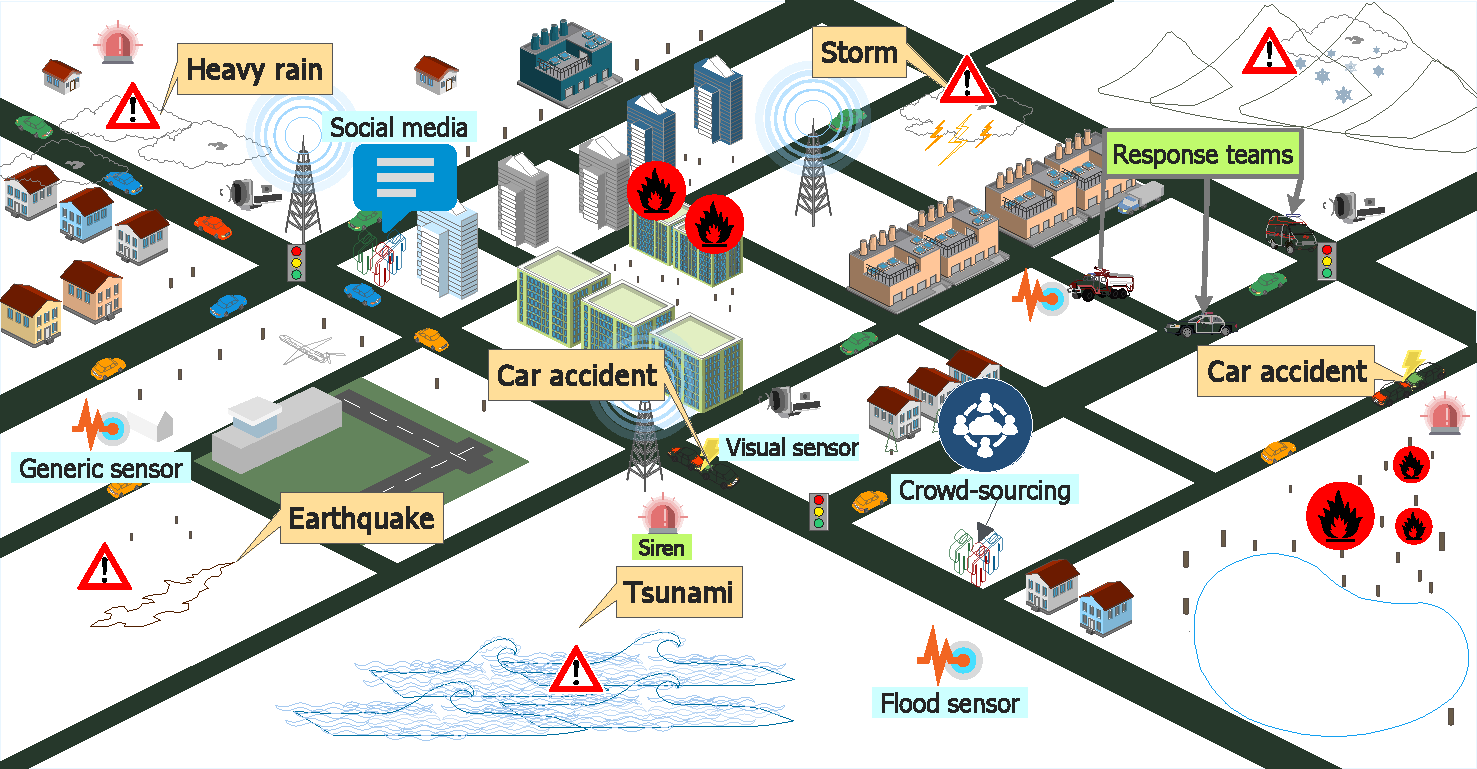
\includegraphics[scale=0.35]{Chapters/1-Survey/images/general.pdf}
\caption{Urban areas: a crisis-prone environment.}\label{Fig:general}
\end{figure}

The contributions of this survey are threefold. First, an emergencies management cycle is defined, classifying and organizing previous works according to their role on it. Second, the fundamentals of the area of emergencies management are established, comprising the concepts of hazards, emergencies, and alarms, which are discussed concerning their effect on the execution of the defined management cycle. Finally, previous works are surveyed and compared using as reference the provided definitions, allowing not only the understanding of the evolution of this area, but also giving clues about open challenges and research directions.

The remainder of this article is organized as follows. Section \ref{sec2} discusses the research context of this article, as well as the adopted methodology for the performed surveying. Section \ref{sec3} discusses the definitions and modelling of the emergencies management cycle and its defining elements. The current panorama of emergency detection is surveyed in Section \ref{sec4}. Section \ref{sec5} addresses alerting services that are executed due to the detection of an emergency. Section \ref{sec6} surveys mitigation actions that can be taken after one or more emergencies are detected in a city. Then, open challenges and research directions are envisioned in Section \ref{sec7}. Finally, conclusions and references are presented.

%%%%% 2 %%%%%%%
\section{Surveying emergencies in smart cities}\label{sec2}

Many aspects were considered when surveying the literature to achieve the expected results in this article. This section highlights the most relevant of such aspects.

%%%
\subsection{The smart service of emergencies management}

When considering the development of research works within the context of smart cities, some concerns may arise due to the nature of such environments. In recent years, smart cities initiatives have been proposed and implemented, embracing new technologies to enhance the citizens' quality of life, potentially making the urban living easier and bringing better management of its resources. Although such objectives seem to be clear, the number and types of complexities that emerge from smart cities initiatives are considerable, raising concerns that may echo and reach the development of emergencies management systems.

Much research efforts have been devoted to transform cities into smart cities \cite{citiestransforming,smartstrategy}. Since this is inherently a multidisciplinary area, researchers have tried to define best practices and engineering procedures to provide smart services in a city, taking into consideration development issues such as sustainability, social responsibility, and energy consumption \cite{citiestransforming2}. As a result, the literature in this area is diverse and potentially huge, covering different subjects comprising multiple views of the same urban environment.

In a typical smart city, several initiatives are devised to make citizens' life better and easier, improving several services such as public transportation, traffic management, water and energy supply, among others. In this sense, emergencies management systems arise as one of the possible services to be provided when defining smart cities, which may even coexist with other parallel services. Making the distinction of this service allow us to better define our scope of research, which will be adopted throughput this article.

At this point, it is worth to mention that although emergencies management systems will be considered in the performed surveying, only the technological aspects of their operations will be discussed. This is intended to help the readability of this article, without overlapping with existing literature in the area.

%%%
\subsection{Adopted surveying methodology}

In order to perform the intended reviewing about emergencies management systems, some criteria were defined. These were obtained from both the scope definition in previous subsection and the selection of some keywords to guide the intended surveying.

It was adopted the Scopus indexing database as reference, since it contains a significant part of the most relevant works in the considered areas, indexing both international journals and conference papers. For that, we adopted the following search queries:

\begin{description}
    \item[Search 1] TITLE-ABS-KEY ( ( "emergency response"  OR  "crisis management"  OR  "crisis model*" )  AND  "smart" )  AND  ( LIMIT-TO ( PUBYEAR ,  2021 )  OR  LIMIT-TO ( PUBYEAR ,  2020 ) OR  LIMIT-TO ( PUBYEAR ,  2019 ) OR  LIMIT-TO ( PUBYEAR ,  2018 )  OR  LIMIT-TO ( PUBYEAR ,  2017 )  OR  LIMIT-TO ( PUBYEAR ,  2016 ) )  AND  ( LIMIT-TO ( DOCTYPE ,  "ar" ) )
    
    \item[Search 2] TITLE-ABS-KEY ( "smart"  AND "emergency"  AND "response"  AND "management")  AND  ( LIMIT-TO ( PUBYEAR ,  2021 )  OR  LIMIT-TO ( PUBYEAR ,  2020 ) OR  LIMIT-TO ( PUBYEAR ,  2019 ) OR  LIMIT-TO ( PUBYEAR ,  2018 )  OR  LIMIT-TO ( PUBYEAR ,  2017 )  OR  LIMIT-TO ( PUBYEAR ,  2016 ) )  AND  ( LIMIT-TO ( DOCTYPE ,  "ar" ) )
\end{description}

In order to have the current picture of the state-of-the-art in emergencies management systems, a six-years window was considered for searching, from 2016 to 2021. The intention was to retrieve the newest relevant papers associated with the keywords \textit{emergencies response}, \textit{emergencies management}, \textit{crisis management}, \textit{crisis models} and \textit{smart cities}.

Considering ``Search 1'', it returned a total of 148 papers and ``Search 2'' returned 113 papers. For each search, title and abstract were manually analyzed to exclude non-related papers. After this filtering, only papers with an average of at least one citation per year were selected. Finally, duplicates were removed. Then, the resulting number of selected works was 51, which was assumed as the reference database when constructing the definitions for emergencies management systems and when comparing the proposed services for detection, alerting, and mitigation. Although a few works outside the defined criteria were eventually considered to support some arguments, all these 51 papers were the core reference for this article, being cited in proper sections according to their contents.

The workflow of the performed searches and papers selection is presented in Figure~\ref{fig:workflow}.

\begin{figure}[htb]
    \centering
    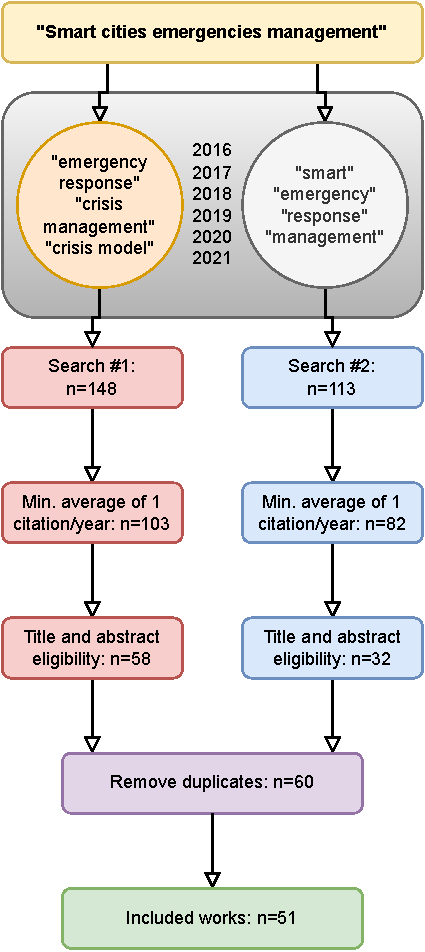
\includegraphics{Chapters/1-Survey/images/fluxograma.pdf}
    \caption{The adopted searching methodology for achieving the core set of works in this survey.}
    \label{fig:workflow}
\end{figure}

%%% 3 %%%%%%%%%%%%%%%%%
\section {The fundamentals of emergencies management systems}
\label{sec3}

The basic function of emergencies management systems in a smart city is the processing of conceptual emergencies along the time in response to detected critical situations. Such emergencies will typically be associated to the causes that created them, influencing the way how emergencies will be alerted and mitigated. Particularly, it is reasonable to say that emergencies will be associated to one or more causes (hazards), as well as to a group of additional information (metadata) that will give more details to support emergencies processing.  

Different methodologies and formalisms have been adopted in the literature when modelling and processing emergencies. However, there are some main characteristics that can be highlighted to better support the understanding of the evolution and current scenario of this research area. Among them, the logical definition of the concept of emergency is described in this section, as well as our proposed classifications for emergencies and emergency-based systems.

\subsection{The emergencies management cycle}

Although definitions may differ when considering the causes and the expected impacts, with some lack of consensus in the literature, it is reasonable to say that an emergency will be an indication of a dangerous situation, requiring proper and immediate action. This way, an emergency may be defined as the beginning of such dangerous situation, when cities may still do something to mitigate it in an attempt to reduce the probability of an emergency to become a disaster. Particularly, a disaster would be the worst consequence of an emergency in terms of inflicted damages, when cities can do little or nothing to mitigate its negative consequences. Hence, it is expected the development of smart city solutions to avoid or delay the occurrence of disasters, ideally diminishing their impacts when they become inevitable. 

Different approaches have defined procedures to handle emergencies and their impacts in urban areas \cite{citiesemergencies1,citiesdisasters1,emergenciesmetric2,mobilityEmergencies1,kumar2017emergency}. Actually, there are many similarities among previous works that allow us to define a generic processing cycle, which can be conceived in a broader concept referred as the ``management'' of emergencies. Such emergencies management cycle would initiate when hazards are perceived as emergencies. This happens when an emergencies detection service identifies that a hazard is being manifested, and this depends on how such service is configured. The detected emergency is then ``virtually'' issued along with all required metadata that is necessary to better understand the emergency and act properly. In the sequence, a notification (alerting/warning) procedure is initiated, informing to all affected and interested elements. Finally, this information processing flow goes to the execution of mitigation actions to cease the emergencies and relieve their impacts. 

Figure \ref{Fig:cycle} depicts this overall emergencies management cycle in smart cities. 

\begin{figure*}[htbp]
\centering
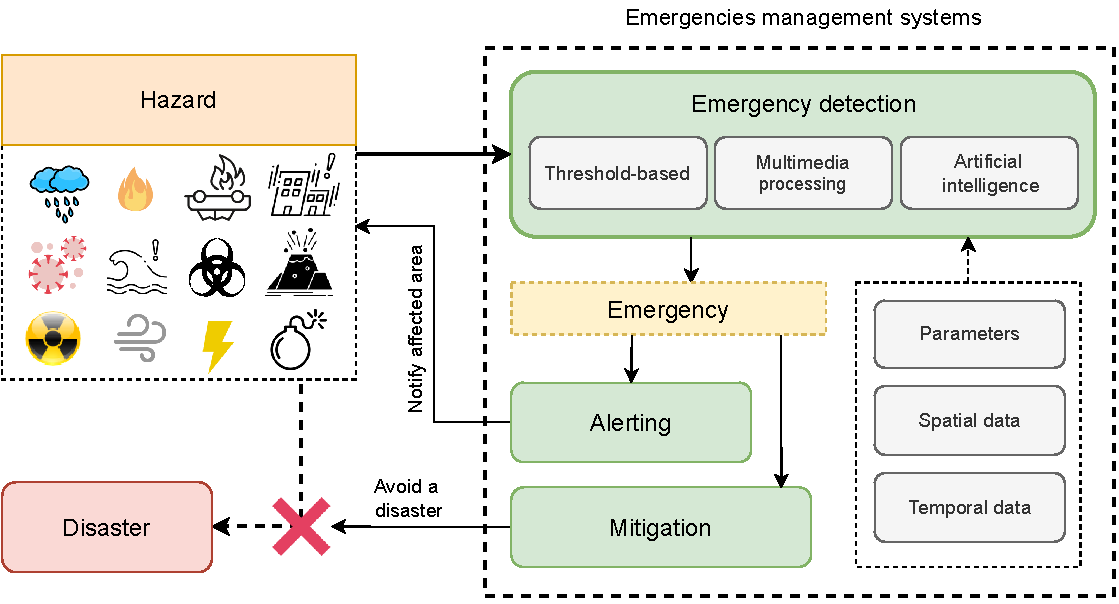
\includegraphics[scale=0.85]{Chapters/1-Survey/images/newcycle.pdf}
\caption{The emergencies management cycle: a hazard is perceived as an emergency to support alerting and mitigation actions.}
\label{Fig:cycle}
\end{figure*}

We consider the following definitions for the elements that compose the proposed emergencies management cycle, described as follows:

\begin{itemize}
    \item \underline{Hazard}: It is the inherent source of danger in an urban environment. In other words, a hazard is a potential cause of a critical situation that may have negative consequences on a city. The hazards will have different origins and behaviors, with different occurrences depending on geographical characteristics and urbanization patterns \cite{hazard1,hazard2}. Although they are the original cause of a disaster, hazards may never happen in a city, while other cities may experience constant critical situations resulted from a single threat \cite{hazard3}. Therefore, in order to properly detect emergencies, hazards have to be continuously monitored;
    
    \item \underline{Emergency}: It is the key element that defines that something is wrong and that something has to be done about it. Usually, an emergency will be a conceptual element that exists within computer-based systems, being created when a hazard is perceived as a current menace and it is detected by some means \cite{socialmedia1,citiesdisasters1}. The objective of an emergency is to provide helpful information to guide the required actions to avoid harmful consequences in a city \cite{emergenciesgeneral1};
    
    \item \underline{Disaster}: It is the ultimate consequence of an emergency that was not tackled by an emergencies management system on time. It is expected that smart cities will treat emergencies in a way that disasters are avoided and thus this is the primary objective of emergencies management systems. However, when untreated emergencies become disasters, some specialized solutions may still be employed, and there are many works in the literature that have addressed particular problems of pre- and post-disaster scenarios \cite{citiesdisasters1,citiesdisasters2};

\end{itemize}

This article is particularly concerned with smart city solutions to handle emergencies before a disaster happens. For that, the defined emergencies management cycle highlights three major processing steps: detection, alerting, and mitigation. All these steps will be discussed in details, as well as the conceptual definitions of emergencies in the literature, encompassing all their complexities. 
%%%%%

%%%
\subsection {Hazards}

In a urban environment, a hazard is any source of potential damage that may harm people or incur in economic losses when it becomes an emergency. Usually, a hazard is perceived as an emergency when it is a current threatening condition, and it ceases to exist when it represents no more risks. This way, for example, the temperature hazard will only become an emergency when it is higher than a safety threshold, or when it is perceived as critical when combined with other hazards. The proper modelling of the hazards is then of paramount importance for this type of applications.

The most usual approach to model and process hazards is to monitor a particular variable along the time. Actually, such approach is easier to implement and may produce very quick responses when employing electronic sensor devices or active data sources. Differently, hazards may be also processed as more complex variables, for example employing cameras \cite{emergenciesmetric3} or artificial intelligence algorithms \cite{emergenciesAI1} to detect hazards that could not be easily identified using individual sensors, generating different types of emergencies. As an example, a fire event could be identified processing still images or processing public posts on social media, potentially providing different types of metadata to support emergencies mitigation actions. Whatever the case, each system will have a particular configuration for hazards monitoring and emergencies detection, according to the characteristics of the target city.

Since the nature of a hazard will dictate how an emergency will be eventually mitigated in a urban environment \cite{citiesdisasters1,hazard2,hazard4}, city-related hazards may be classified into three different groups: Environmental, Urban and Health. Environmental hazards are those resulted from natural conditions that may affect a city, such as heavy rain, hurricanes, earthquakes, volcano eruptions, among others. The other two types of hazards, Urban and Health, are both causes of human-induced disasters. We propose to subdivide them into two different groups due to the expected relevance that outbreaks surveillance and detection systems should assume in the development of smart cities \cite{covidsmartcities1,covidsmartcities2,enviroment3}. This way, Urban hazards will be related to the way we live in cities, with increasing overpopulated areas and crowded mobility systems, resulting in hazards related to traffic accidents, house firing, gas explosion, building collapsing, terrorist attacks, violent protests, robbery, etc. Finally, Health hazards will not only be associated to individual health emergencies, such as heart attacks, but collective threats due to the spread of infectious diseases. Figure \ref{Fig:hazards} presents a comprehensive organization of the expected hazards in urban areas. 

\begin{figure*}[htbp]
\centering
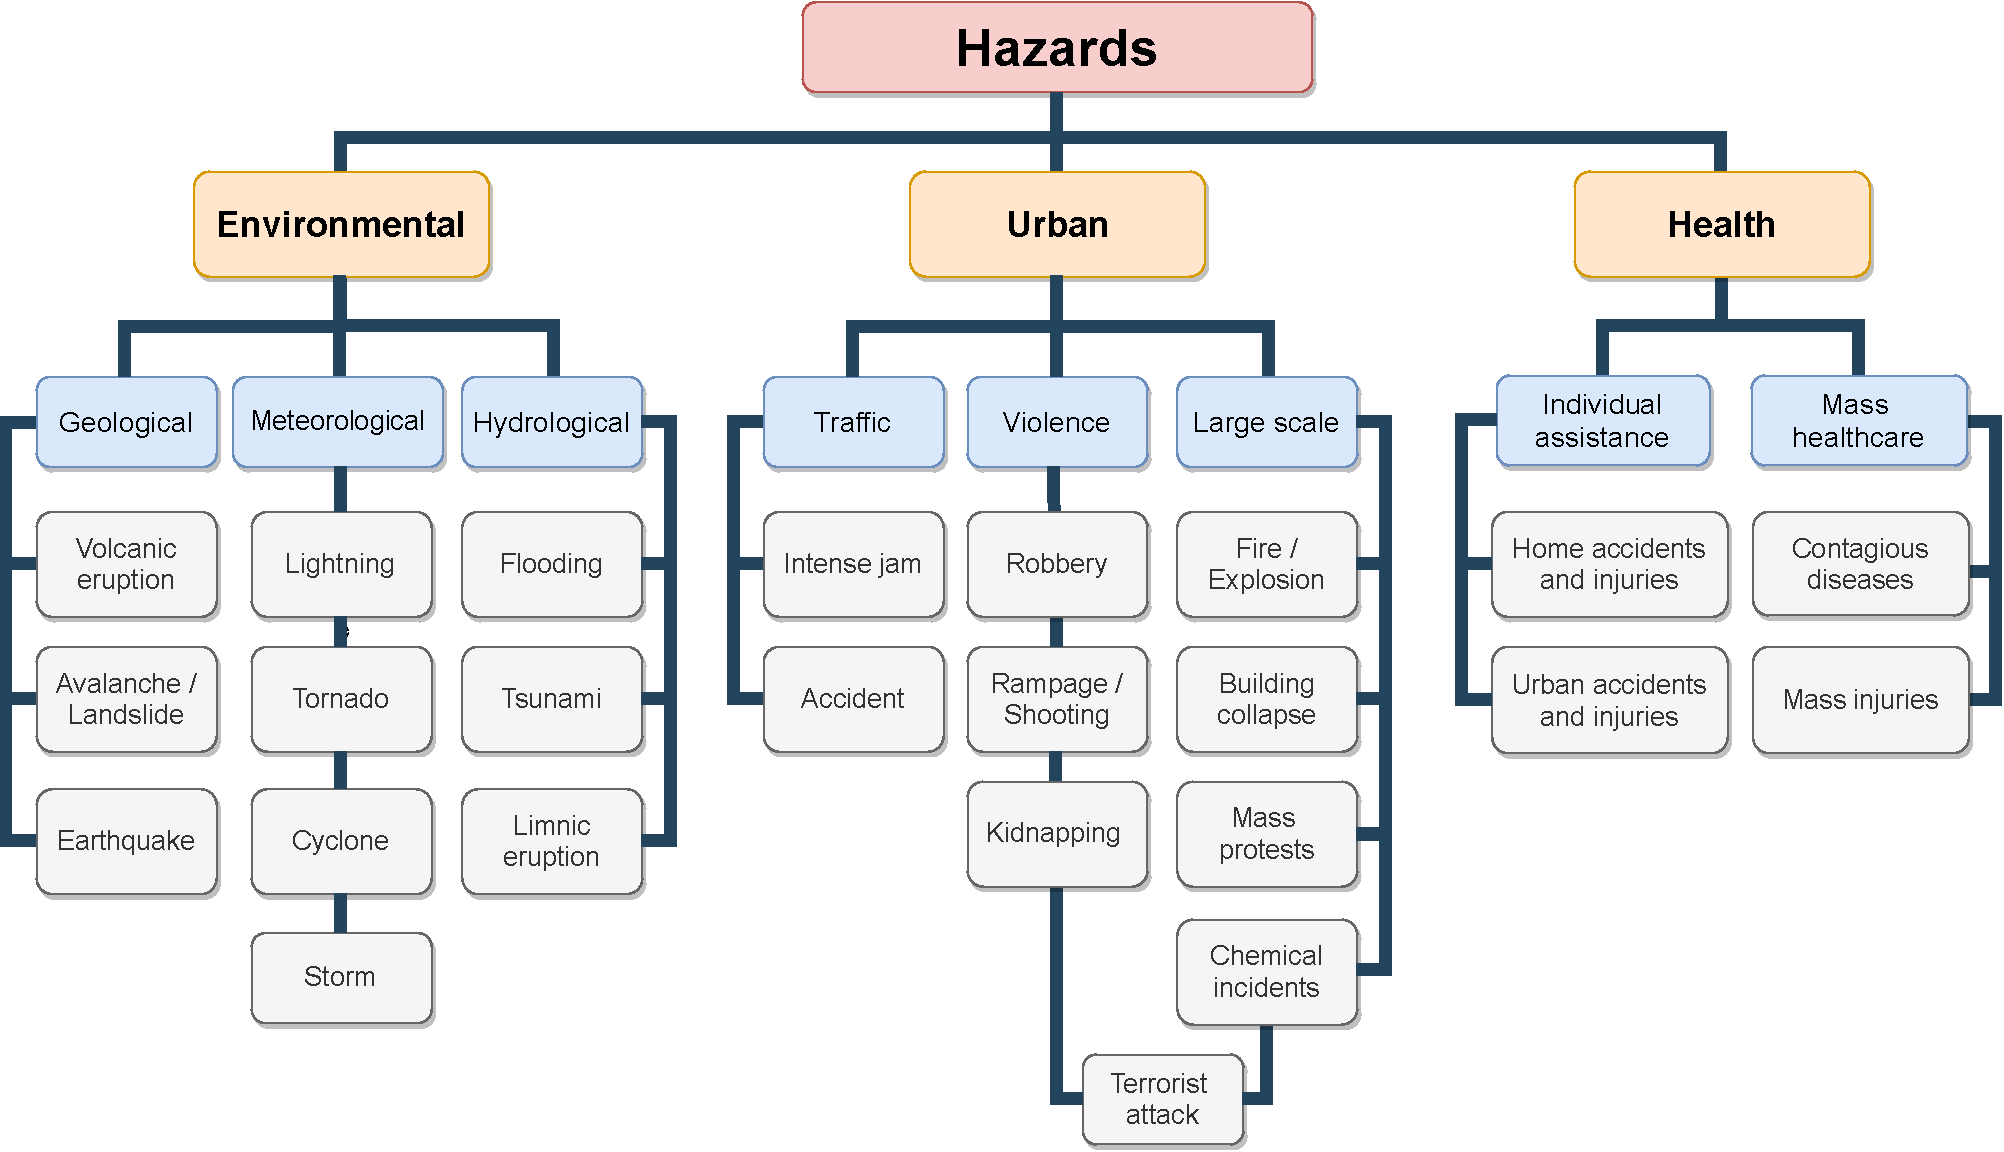
\includegraphics[width=\linewidth]{Chapters/1-Survey/images/Hazards.pdf}
\caption{The proposed classification and some common hazards in modern cities.}
\label{Fig:hazards}
\end{figure*}

Human-induced disasters may result in infrastructural damages, injuries and deaths. Although there is not a straight line between the frequency of Urban and Health hazards and the urbanization process, the urban sprawl in this century will result in more large and mega cities around the world, with potential for higher number of disasters \cite{urbansprawl1,urbansprawl2}. In parallel, climate changes are strengthening the destructive power of natural disasters, putting additional pressure on emergencies management systems \cite{enviroment1,enviroment2}. As a result, the last decades have seen an increasing in the number of emergencies detection approaches, focusing on different types of hazards. 

%%%%
\subsection{Defining and modelling emergencies}

Emergencies are defined as a virtual entity that comprises one or more hazards and a group of metadata. Hence, for emergencies detection systems, a major issue will be to define how coupled are the emergencies concerning their associated hazards, which lead us to propose two different classifications for the definition of emergencies:

\begin{itemize}
    \item \underline{Self-contained emergencies}: Since emergencies are critical situations that may cause damages, injuries and deaths, many approaches have focused on handling them as self-contained critical elements. In such cases, an emergency is associated to a single hazard, resulting in emergencies being a result of a single cause. This way, for example, there are Earthquake Emergencies, Fire Emergencies, Flooding Emergencies and Traffic Emergencies. For some solutions targeted at a single type of emergency, such as the work in \cite{iotFire1} for fire emergencies and the work in \cite{iotRain1} for heavy rain emergencies, the proposed system is usually deployed to detect a particular type of hazard. Differently, other approaches provide some level of flexibility, allowing the detection of different hazards, but the eventual issue of an emergency is still associated with a specific type of hazard, as in \cite{emergenciesmetric4}. Whatever the case, the processing of self-contained emergencies (also referred as atomic emergencies \cite{emergenciesmetric6}) has been adopted as a simpler way to issue and handle emergencies that have the characteristics of their single associated hazards;
    
    \item \underline{Events-based emergencies}: For some systems, each manifested hazard will be processed as individual critical events, which will be independent indications that something critical is happening or about to happen. In this perspective, an emergency will be the conjunction of one or more events, acting then as a ``container'' of manifested hazards. For such systems, the separation between events and emergencies allow a more structured processing of critical situations, since emergencies can be defined as a composition of multiple critical events that may give more detailed clues about what is happening at a certain place and time.
\end{itemize}

Since events-based emergencies may be too complex when considering all the possibilities in smart city scenarios, we also classify it into two different subgroups, defined as follows:

\begin{itemize}
    \item Triggered emergencies: It happens when thresholds are exploited to trigger the detection of an emergency. Overall, this is a simpler way to detect emergencies, since thresholds can be defined for a group of hazards monitored by sensors or other data source. In \cite{emergenciesmetric2}, an event of interest is associated to a scalar metric measured by a sensor, and each event of interest is triggered when the measured values are higher (or lower) than defined thresholds. Then, all triggered events are used to compose a single emergency. As an example, for a temperature threshold of $50^{\circ}$C, an emergency is detected when the measured temperature is higher than that reference value, but other types of hazards may also compose the same detected emergency;
    
    \item Aggregated emergencies: For a particular group of emergencies management systems, emergencies will be detected not by triggering and safety thresholds, but by the combined processing of multiple monitored hazards. In these cases, multiple hazards are monitored and considered for the detection of emergencies, in a combined way, creating either separate emergencies or combined macro-events emergencies, depending on the characteristics of the implemented system. For such group of emergencies, multimedia processing algorithms and artificial intelligence can be employed to combine multiple data from monitored hazards, exploiting techniques and algorithms in areas such as visual computing, audio processing, machine learning, genetic computing and fuzzy logic. The work in \cite{SultanMahmud2017} makes use of machine learning algorithms to read several sensors and generate a fire danger level instead of just monitoring thresholds. Images of the monitored area are also interpreted by machine learning algorithms to better define if there is a fire emergency or not. Another relevant scenario for such type of processing and modelling is the early detection of emergencies using machine learning, when the combined perception of the behavior of the expected hazards indicate that something may soon become wrong \cite{machine1}. Such solutions could be even exploited to support a different class of applications in the area of emergencies avoidance, as already largely adopted for traffic avoidance in Intelligent Transportation Systems (ITS) \cite{machine2}.
\end{itemize}

It is important to notice that hazards are the original causes of emergencies, thus indicating their nature. This way, for example, an emergency issued due to a temperature hazard may suggest the dispatching of fire trucks, while an emergency issued after a traffic accident may be handled by adjusting traffic lights. Therefore, understanding the possible hazards in a city is crucial when managing emergencies. 

Table \ref{Tab:hazards} summarizes some works in the literature concerned with emergencies, highlighting their characteristics according to the modelling of hazards.

\begin{table*}
\centering
\caption{Research works and the modelling of hazards and emergencies.}
\label{Tab:hazards}
\begin{tabular}{|c|c|c|c|c|c|c|c|}
    \multirow{2}{*}{\textbf{Work}} & \multirow{2}{*}{\textbf{Year}} & 
    \multicolumn{3}{|c|}{\textbf{Hazards}} & \multicolumn{3}{|c|}{\textbf{Emergencies}}\\
    \cline{3-8}
    & & Environ. & Urban & Health & Self-contained & Triggered & Aggregated \\ 
    
    \hline
    \citeauthor{emergencyTraffic1} \cite{emergencyTraffic1} & 2012 &  & vehicular sensors & & X & & \\
    
    \hline
    \citeauthor{detectionAudio1} \cite{detectionAudio1} & 2013 &  & audio & & X & & \\
    
    \hline
    \citeauthor{iotRain1} \cite{iotRain1} & 2016 & rain &  &  & X & & \\
    
    \hline
    \citeauthor{SultanMahmud2017} \cite{SultanMahmud2017} & 2017 & fire & fire & & & & X \\
    
    \hline
    \citeauthor{iotDetection2} \cite{iotDetection2} & 2017 & multiple data & multiple data & multiple data & & X & \\
    
    \hline
    \citeauthor{iotDetection1} \cite{iotDetection1} & 2018 & multiple data & multiple data & multiple data &  & X & \\
    
    \hline
    \citeauthor{iotFlood1} \cite{iotFlood1} & 2018 & water & water & & X & & \\
    
    \hline
    \citeauthor{iotFire1} \cite{iotFire1} & 2018 &  & gas, smoke, temperature & & X & & \\
    
    \hline
    \citeauthor{iotPollution1} \cite{iotPollution1} & 2019 & air pollution & & & X & & \\
    
    \hline
    \citeauthor{Alkhatib2019771} \cite{Alkhatib2019771} & 2019 & & multiple data & & & & X \\
    
    \hline
    \citeauthor{BRAGAGNOLO2020104240} \cite{BRAGAGNOLO2020104240} & 2020 & landslide & & & & & X \\
    
    \hline
    \citeauthor{emergenciesmetric2} \cite{emergenciesmetric2} & 2020 & multiple data & multiple data &  multiple data &  & X & \\
    
    \hline
    \citeauthor{emergenciesmetric3} \cite{emergenciesmetric3} & 2020 & multimedia data & multimedia data & multimedia data &  & X &\\
    \hline
    
    \citeauthor{iotCovid1} \cite{iotCovid1} & 2020 &  & visual data &  & X & & \\
    \hline
    \citeauthor{iotEarthquake1} \cite{iotEarthquake1} & 2020 & earthquake &  &  & X & & \\
    \hline
    
    \citeauthor{twitterDetection1} \cite{twitterDetection1} & 2020 & social media & social media &  social media &  & X & \\
    
    \hline
    \citeauthor{fireBigdata1} \cite{fireBigdata1} & 2021 & fire & fire & & & & X \\
    
\end{tabular}
\end{table*}

%%%%%%%%%%%%
\subsection {Associating metadata to the emergencies}

When an emergency is detected within an emergencies management system, it is virtually created to be further processed. Such emergencies will be typically associated to a group of metadata, providing different types of information. Although there may be different types of metadata associated to emergencies, we identified three major groups that will be mostly considered when handling emergencies, defined as follows.

\subsubsection{Affected area}

An emergency will usually be assumed to occur in the same area of its cause (one or more hazards), which is defined as its ``area of incidence''. This is usually a point on a city that may be located on public or private areas, depending on the adopted approach and the monitored hazards. Actually, although it may be reasonable to use relative positions in a urban environment, or even Cartesian coordinates according to a reference point, many approaches will employ GPS (Global Positioning System) coordinates to precisely locate the areas of incidence of detected emergencies. Actually, the adoption of GPS coordinates has led many approaches to exploit sensor units equipped with GPS devices \cite{smartsensing1} or to use GPS-enabled smartphones when harnessing crowdsourcing algorithms \cite{smartsensing2}.

In fact, the location of the detected hazards will be the reference position of the corresponding emergency, but some approaches may also assume that an emergency will be felt in an area irradiating from that location. That ``influence zone'' may be modelled in different ways, although it will be often processed as a circular area with the area of incidence as the center of that circumference \cite{s150614370}. Additionally, as an important remark, two different hazards may be associated as belonging to the same emergency if they are being detected within a certain area not greater than some defined tolerable distance. Obviously, it will be a function of the desired precision, since two different hazards detected in the same block or street could be processed as the same emergency for practical reasons.

It is worth to mention that a wider influence zone may be defined according to the type of the detected hazard and the affected area. For example, a fire hazard in a neighborhood with many wooden houses may be too critical because the fire may rapidly spread, specially under windy conditions (which may be also processed as a hazard) during a dry season (a temporal significance of the emergency, as further discussed in this article) \cite{iotFire2}. In such cases, the initially detected emergency may have a wider influence zone, for example allowing preventive evacuation \cite{evacuation}.

%%%%%%%
\subsubsection{The duration of emergencies}

Since all emergencies will be associated to at least one hazard, a particular emergency is issued when an associated hazard is considered to be manifested in an area, either because a corresponding event was triggered or due to some aggregated processing of multiple hazards. Whatever the case, although the cause of an emergency may rapidly cease, for example in an earthquake, its effects may endure for a longer time, threatening people in different ways. For example, the impacts of an emergency composed of both earthquake and tsunami hazards may be sensed for days or weeks, even if those hazards persist in a critical level for just a few minutes \cite{tsunami1}. This way, emergencies management systems should be aware that emergencies may have different temporal behaviors, which may be affected by the type of hazards and by the social, economical and spatial characteristics of the considered city.

Actually, there is a gray area in the literature considering how critical situations persist in a city. In some perspectives, a critical situation that last for some time may be considered as a pre-disaster  
period \cite{citiesdisasters2,citiesdisasters3} or even a post-disaster situation \cite{citiesdisasters4,citiesdisasters5}. On the other hand, the duration of a critical situation may roughly be the duration of an emergency that can still be addressed before a disaster is formally defined, as expressed in the management cycle in Figure \ref{Fig:cycle}. Although there is not a consensus about the temporal significance of emergencies and disaster configurations, this article is mostly concerned with the duration of emergencies that can still be mitigated by some computer-assisted system.  

Therefore, for many emergencies detection approaches, an emergency will last for some time even after the original hazard stop being critical, benefiting mitigation actions as the assignment of emergency response teams. For the work in \cite{emergenciesmetric2}, that duration depends on each mitigation approach, which could assume any duration after an emergency stop being reported. Also, an algorithm is proposed in that work to model a temporal significance of emergencies that slowly decreases over time, which may be quite realistic for some types of hazards. In other perspectives, such as in \cite{socialmedia1,emergenciesmetric4,emergenciestimemedia}, emergencies can be assumed as active as long as their causing hazards are being perceived as critical. The modelling of the duration of emergencies is then an important project characteristic, with a lot of practical implications.

%%%
\subsubsection{Computing severity levels} 

Emergencies will be detected at a certain position, having an influence zone and lasting for some time. Although all this metadata is relevant to understand and to model emergencies, their real potential to cause destruction, injuries and deaths may rely on other types of parameters. Actually, such potential of destruction, generically measured as the ``severity level'' of an emergency, may be a function of many variables besides the hazards that created it.

In general, we can expect that self-contained emergencies will rely on the magnitude of the monitored hazards, while events-based emergencies would exploit other types of information to indicate their level of criticality. Considering the proposed approaches in the literature, in different scopes, we have identified different groups of parameters to be used when computing a severity level for the emergencies, which are summarized as follows:

\begin{itemize}
    \item Hazard significance: Since emergencies will be associated to one or more hazards, it is natural to compute the severity level based on the characteristics of the hazards that compose them. However, there are different characteristics to be accounted, resulting in different ways to compute such level. For threshold-based approaches, hazards are processed as ON/OFF events and thus the severity level is only impacted by the number of triggered events that compose the considered emergency \cite{emergenciesmetric2}, or simply by the manifestation of the hazard itself \cite{emergenciesmetric4}. In such cases, a hazard is already something critical, and there is no hazard that is more critical than other hazard of the same type \cite{emergenciesmetric2}. On the other hand, the ``intensity'' of a hazard may also impact the criticality of an emergency, and two temperature hazards originated from different sensed temperatures will account differently when computing the severity level;
    
    \item Spatial significance: The areas of incidence and the influence zone are useful information to indicate where mitigation procedures can be taken to save lives and reduce damages. That information may be already present as metadata of emergencies and thus it seems natural to exploit them to enhance the computation of the severity level. In fact, the potential of negative impacts may be a function of the area under an emergency in a city, and different parameters may be considered for that. Actually, the inherent risk of damages in an area may be accounted based on the 1) the spatial composition and organization of the buildings and infrastructure, and 2) the population density and mobility patterns in a city. For example, an area with many wooden houses may have an innate risk \cite{firespatial1} and thus a fire emergency in such a region should be more critical for a city as a whole \cite{firespatial2}, potentially leading to the necessity of some prioritization when dispatching fire trucks to attend that emergency \cite{costa2020automatic}. In a different perspective, areas with high population density in large cities may also suffer more from the same emergency when compared to low populated areas in the suburbs \cite{firespatial3}. Since such population density may vary along the time, according to urban mobility patterns \cite{mobilityEmergencies1}, it is also reasonable to apply dynamic mechanisms to compute the severity level according to how people move within a city;

    \item Temporal significance: The third element that might be accounted when computing the severity level is the temporal significance associated to the affected area. Actually, when an emergency is happening is very important since its negative effects may be boosted or attenuated according to movement patterns and the availability of mobility services along the days, weeks and months. In this sense, holidays and weekends may impact the emergency severity level, as well as hush hours in weekdays. In \cite{firetemporaldata1}, statistical analysis of fire concerning the time of the day, the day of the week and the month of the year are performed, associating temporal data with the impact of fire hazards. For the work in \cite{hurricanetemporal1}, multiple data are combined to estimate the impacts of hurricanes, predicting their trajectory. Then, other emergencies in a city would have higher levels of criticality if they occur during a hurricane season. In other example, crime incidents during the day, night and dawn could be used to classify emergencies \cite{crimetemporal1}, specially when related with urban hazards. In all these cases, temporal modelling would provide additional data to support the assessment of the severity level of the emergencies.

\end{itemize}

There are important remarks when computing the severity level of emergencies and the literature has presented interesting solutions when handling them. In general, it is reasonable to say that the monitored hazards and the expected outcomes of the employed systems will strongly dictate how severity will be computed. For the work in \cite{iotEarthquake2}, multiple sensors are used to gather information about acceleration and vibration, which is used to detect earthquakes. A warning message (emergency) emitted by that system is classified into one of three different levels, according to the detected shaking intensity. However, a different approach would be to assume that any earthquake with a magnitude higher than a certain threshold would already be a critical situation. For the work in \cite{iotEarthquake3}, a sensor network is used to detect earthquake emergencies, which are issued when a seismic peak is detected. In that case, all hazards have the same severity level. But since the hazard is an earthquake, it is already a threatening condition and thus giving a severity level to it may be pointless for some applications (a detected earthquake is already bad enough when it is higher that a ``safety'' level).

Another interesting remark is that the definitions of the impacts of spatial metadata of an emergency may vary considerably, depending on the developed system and the target city. In this sense, a downtown area with many hospitals and schools may be more severely affected by the same type of emergency in the suburbs, but the other way around is also possible if there are critical chemistry industries at the suburbs. The lack of efficient mobility may also impact emergency vehicles, which would be dispatched from some fixed stations (e.g. a fire department). In fact, such spatial significance may be not easy to be defined, demanding proper modelling.

It is also worth saying that some types of hazards are hard to graduate within a scale. In a traffic accident, for example, it may be meaningless to account the number of involved cars, since the number of victims may be a more desired information to be considered. The same reflections can be made for other urban or health hazards. Actually, many emergencies systems related to such hazards have implemented crowdsensing approaches to detect them, which make it hard to compute severity levels based on the hazard nature. Particularly, it is better to classify all these emergencies as equally critical, relaying on other parameters to compute levels of criticality. In \cite{emergenciesmetric3}, the severity level of events-based triggered emergencies is a direct function of the number of detected hazards. However, since there are some hazards that may provide more information about a particular critical situation, that work assigns twice the relevance for hazards detected using cameras and visual processing algorithms, when compared to hazards detected by scalar sensors. For example, if a building is on fire, a camera may detect a fire emergency which is twice as relevant as temperature or smoke emergencies. Nevertheless, in that work, all emergencies resulted from the same type of cause (hazard) will still have the same impact on the severity level, regardless of their sensed intensity or magnitude. 

The final objective of giving an impact level to the emergencies is to support decision algorithms when handling multiple concurrent emergencies. Since many cities may have finite resources to attend emergencies, for example concerning the availability of emergency vehicles and response teams \cite{costa2020automatic,tsunami1}, such severity assessment may be an important element for emergencies management systems. Once again, each city may have particular temporal and spatial significance, which may be associated with its sub-regions and neighborhoods. Therefore, proper modelling of such characteristics would be worth when computing all metadata related to emergencies in a city, improving the effectiveness of the employed systems and the alerting and mitigation procedures.

%%%%%%%%%%%%%%%%%%%%%%%%%%%%%%%%%%
%%% 4 %%%%%%%%%%%%%%%%%
\section{Detecting emergencies}
\label{sec4}

When reviewing previous works in the research area of smart emergencies management, particularly when concerning to the detection of emergencies, it is possible to sort out three major sources of data: sensors, crowdsourcing and big data. Sensors will be used to directly monitor one or more hazards, as close as possible to the affected area. Crowdsourcing will use a different paradigm, indirectly collecting data from multiple sensors, gadgets and even people to perceive a critical situation. Finally, big data approaches will usually process data from multiple sources not necessarily related to the monitored hazards, even considering data of historical occurrence of emergencies in an area. 

The detection of emergencies may then be performed in multiple ways and the literature has also presented some interesting solutions about the detection and the issuing of emergencies exploiting very different data sources. Actually, although such sources may differ concerning characteristics as availability, scalability, cost and accuracy, it is usually expected the definition of at least one Emergencies Detection Unit (EDU) to perform detection functions, even in a more generic way, which will have a well-defined data input, one or more processing algorithms and some additional configurations for the emergencies (metadata). EDUs may be implemented on electronic components ``on the edge'' (closer to the hazards) \cite{PlatformsSC,sensorsplatforms}, on central computers \cite{twitterDetection2,centralserver1} or even exploiting cloud-based services \cite{cloud1}, either taking a single input data stream or having multiple data sources at once. 

Figure \ref{Fig:detection} depicts a generic scheme for the detection of emergencies in smart cities. 

\begin{figure}[ht]
\centering
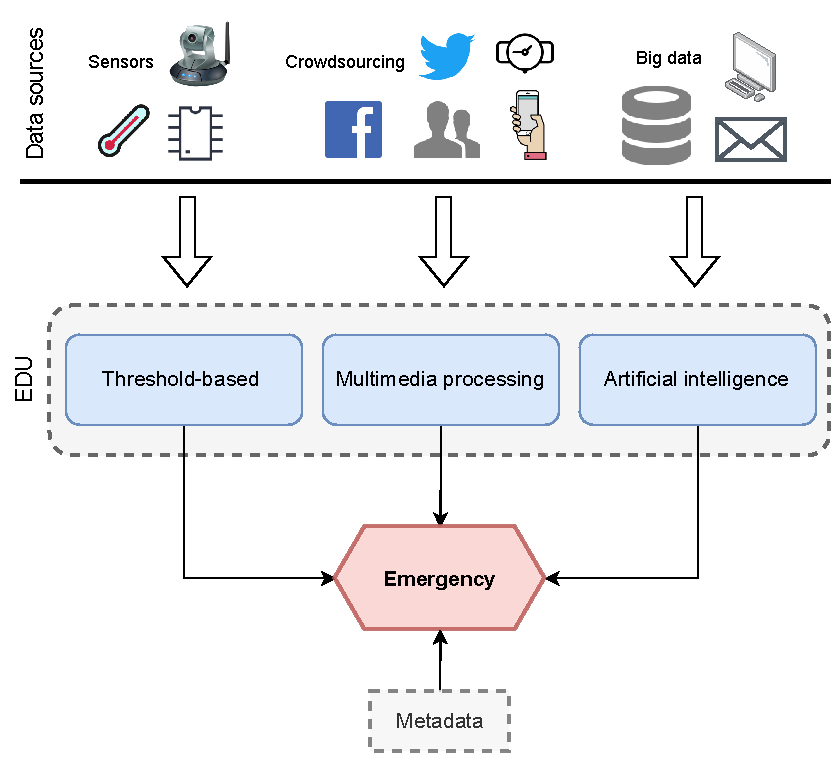
\includegraphics[scale=0.6]{Chapters/1-Survey/images/detection.pdf}
\caption{Detecting emergencies through the monitoring of hazards in a city, considering different sources of data.}
\label{Fig:detection}
\end{figure}

%%%
\subsection{Input data sources}

The detection of emergencies should exploit different sources of data in order to take more accurate decisions. However, characteristics of the employed approaches and the particularities of the target city will dictate the best (and more affordable) data sources to be considered. Therefore, in order to better understand how they could be used in practical applications, the three major sources of data for emergencies detection are discussed in next subsections.

%%
\subsubsection{Electronic sensors and sensor networks}

The most direct way to detect emergencies is to employ sensor devices to monitor a particular hazard along the time. Such electronic components are able to measure a particular variable, which can be processed locally \cite{edge1} or transmitted to other devices for further processing \cite{iotRain1}. Additionally, while sensors may be exploited to detect a specific group of hazards (fire, pollution, rain, flooding, gunshots, etc), it is also possible to employ them to support adjustable architectures to monitor any groups of hazards and emergencies \cite{emergenciesmetric2,emergenciesmetric4,emergenciesmetric6,emergenciesmetric5}. Whatever the case, sensors will provide scalar or multimedia data to be further processed by any detection algorithms.

When implementing the generic concept of an EDU, sensors may be attached to an electronic processing board that will handle all sensing activities, as well as the networking and data processing functions expected from it. Such boards may have a continuous energy supply or they may be powered by batteries \cite{energy1}, affecting the deployment planning of the EDUs and their mobility patterns. In fact, the proper choosing of the hardware and software characteristics of the employed sensors and the associated central processing unit has proven to be an important project decision of computer-assisted solutions for emergencies detection, with important developments in recent years \cite{sensorsplatforms,sensorsplatforms2,sensorsplatforms3}.

The use of sensors to detect emergencies has maturated along with the evolution of Wireless Sensor Networks (WSN) \cite{surveywsn2}. Since the beginning of WSN developments, sensors had being harnessed to monitor critical zones as factories, furnaces, nuclear reactors and several equipment that could bring danger to people and nearby facilities. With the emerging concepts of Internet of Things (IoT) and smart cities, sensors are now perceived in a broader perspective that comprises virtually anything in a urban environment \cite{smartsensing1,smartsensing3}. This flexibility, together with the increasing affordably of powerful electronic boards for open source and open hardware developments \cite{PlatformsSC}, have not only transformed the way smart cities have been created, but also how emergencies can be better managed on modern cities. Therefore, the adoption of sensors-based emergencies detection units is the culminating point of a continuous evolution process. 

Table \ref{Tab:sensorsbased} summarizes previous works in the literature that employ one or more sensor devices to support the detection of emergencies.

%% Table
\begin{table*}
\centering
\caption{Sensors-based detection of emergencies.}
\label{Tab:sensorsbased}
\begin{tabular}{|c|c|c|c|c|}
    \textbf{Work} & \textbf{Year} & \textbf{Hazard} & \textbf{Sensors} & \textbf{Processing hardware}\\

    \hline
    \citeauthor{iotRain1} \cite{iotRain1} & 2016 & rain & air pressure, temperature, humidity, wind speed, solar & Raspberry Pi 2 \\

    \hline
    \citeauthor{iotRain2} \cite{iotRain2} & 2016 & extreme weather & air pressure, humidity, wind speed and direction & Arduino Uno \\
    
    \hline
    \citeauthor{iotFire4} \cite{iotFire4} & 2017 & fire & smoke, gas, flame & ESP 32\\
    
    \hline
    \citeauthor{iotRadiation1} \cite{iotRadiation1} & 2017 & radiation & radiation & BeagleBone Black \\
    
    \hline
    \citeauthor{iotFire1} \cite{iotFire1} &  2018 & fire & smoke, gas, temperature & not specified \\

    \hline
    \citeauthor{iotPollution1} \cite{iotPollution1} & 2019 & air pollution & gas & Arduino \\
    
    \hline
    \citeauthor{iotAudio1} \cite{iotAudio1} & 2019 & gunshots & audio & Rasbberry Pi 3 \\
    
    \hline
    \citeauthor{ThresholdBasedFallDetection2019} \cite{ThresholdBasedFallDetection2019} & 2019 & fall detection & accelerometer & smartphone \\
    
    \hline
    \citeauthor{visualdataEmergency5} \cite{visualdataEmergency5} & 2019 & violent behavior & visual sensor & Raspberry Pi 3 \\
    
    \hline
    \citeauthor{iotBike1} \cite{iotBike1} & 2021 & dangerous ambient conditions & temperature, humidty, UV radiation, pollution & Raspberry Pi Zero W \\
    
    \hline
    \citeauthor{iotFire3} \cite{iotFire3} & 2021 & fire & smoke, gas, temperature & ATMEGA328P\\
    
    \hline
    \citeauthor{CarCrash2021} \cite{CarCrash2021} & 2021 & vehicle emergency (car crash) & motion, vibration & Raspberry Pi 3 \\
    
    \hline
    \citeauthor{earthquakesDetection2011} \cite{earthquakesDetection2011} & 2021 & earthquakes &  accelerometer & Cloud (Google App Engine) \\
    
\end{tabular}
\end{table*}

An important remark about the detection of emergencies is the level of reliability we may have concerning this entire process. And such reliability may be associated to different aspects with particular challenges. In first place, sensors may fail, compromising the quick detection of emergencies \cite{availability1,availability2}. Moreover, the network may also fail, delaying or even forbidding the delivery of emergency alerts \cite{networking1,networking2}.
In such cases, in order to improve the expected detection quality when employing networks of sensor nodes, different strategies can be taken, such as sensors redundancy \cite{redundancy2}, transmissions reliability \cite{reliability1} and fault tolerance in sensor networks \cite{redundancy1}. 

A second concern is the prioritization of sensor nodes. In a urban scenario, some sensors may be more relevant than the others based on different criteria (position, sensing configuration, energy resources, transmission bandwidth, etc), and thus data retrieved from them may be assumed as more relevant or having higher associated Quality of Service (QoS) / Quality of Experience (QoE) \cite{smartcities3,priority1,qoe1}. This fact may be exploited to develop emergencies detection systems that are better adapted to support quick and more accurate detection on more critical areas of a city \cite{priority4}. In \cite{priority2}, when an emergency is detected, cameras are turned on to provide more detailed information about the affected area, becoming themselves more relevant nodes for the network. A similar strategy is proposed in \cite{priority3}. Actually, this principle of more critical monitoring can be extended even further, considering for example how sensor nodes will access the networks to deliver emergency alarms \cite{qosnetworks1} or how they will be deployed on a urban area \cite{deployment1}. Nevertheless, although beneficial when better addressing rapid detection procedures on more critical areas, prioritization approaches may compromise the effectiveness of emergencies detection from less relevant nodes. Hence, the prioritization of sensor nodes should be carefully adopted to avoid detection blackouts. In this sense, the most suitable approaches seem to be the ones that adopt dynamic assignments of priority for the sensors, especially when assuring some level of fairness \cite{smartcities3}.   

%%%
\subsubsection{Crowdsourcing}

Hazards may also be monitored in a more distributed and cooperative way. Although sensors may be used to collectively provide data, for example when sensors embedded in smartphones are used, the concept of crowdsourcing (or crowdsensing) is mostly based on the premise that the number and position of contributors may change continuously, whatever is the actual source of data (sensors, posts on social media, asynchronous georeferenced messages, etc) \cite{crowdsourcing2}. In fact, this principle has been exploited by many applications that need collaborative data acquisition and processing in a city, such as in traffic \cite{citiesvehicles2} and environmental monitoring \cite{bikesensor}, but its adoption for emergencies detection may also bring significant results. 

Crowdsourcing will provide data in a urban scenario exploiting different technologies and platforms, which may be valuable when providing heterogeneous data \cite{crowdsourcing6}. Moreover, since the technological infrastructure of already existing systems and applications are often leveraged when implementing emergencies-centric crowdsourcing approaches, they tend to cost less and take fewer time to be get operational. This combination is highly beneficial when facing the stringent challenges of efficient emergencies detection in urban areas.

Previous works in the literature have exploited three major groups of crowdsourcing approaches according to the considered source of data. Such groups are described as follows:  

\begin{itemize}

    \item Social media: People make millions of interactions, status updates and multimedia posts daily on different social media platforms, comprising photos, videos, and a lot of textual information \cite{socialmedia2}. Such data can be ``mined'' and processed to detect emergencies in a city, with a lot of promising applications taking advantage of the inherent characteristics of social media posts. In \cite{socialmedia3}, geotagged public tweets (textual posts on the Twitter microblogging service) are processed to detect traffic incidents in a city, continuously. For the work in \cite{twitter4}, tweets are processed to detect emergencies in a smart campus scenario. In that work, tweets are classified into four different groups: Mobility, Fire, Health and None (no event), according to the perceived patterns. Actually, processing of textual information will comprise at least the identification of keywords and language patterns \cite{twitter1}, but some particular challenges may also exist when detecting emergencies in a smart city, such as time efficiency and accuracy \cite{socialmediatime1}. Furthermore, in order to improve emergencies detection procedures, multimedia data on social media may also be processed for this purpose, but the additional processing costs should be accounted. In \cite{crowdsourcing5}, a crowdsourcing approach is adopted to share visual data describing potential emergencies, which are spontaneously provided by the inhabitants using a posting platform, supporting the detection of emergencies in a city by centralized algorithms. Similarly, the work in \cite{crowdsourcing7} also processes images to detect emergencies, but exploiting visual data on popular social media instead. Overall, the processing of social media posts may give important clues about emergencies, specially in crowded cities with many active social media users \cite{socialmedia4,twitter4};
    
    \item Smartphones and wearable sensors: Since smartphones became very popular in the last decades, as almost every person carries a smartphone nowadays as a multi-purpose portable tool, it is very reasonable to adopt them as a platform for crowdsourcing \cite{crowdsourcing1}. In parallel, a revolution of wearable sensors has also taken place more recently, particularly with the popularization of smartwatches and healthcare gadgets, also providing valuable collaborative data to be processed \cite{wearable1,wearable2,iotgadget1}. Modern smartphones and popular gadgets are equipped with a myriad of embedded sensors, a GPS receiver, rechargeable batteries with decent energy capacity, and networking capabilities (Wi-Fi, Bluetooth, 4G/5G). Hence, they are inherent mobile sensor units that can provide data for multiple concurrent applications, even in a transparent way for the users. In \cite{crowdsourcing4}, authors propose an emergencies detection mechanism using smartphones, along with data from the embedded accelerometer sensor and its GPS. With that data it is possible to detect if the person (user) is walking, running, falling or laying on the floor, indirectly supporting in the identification of a critical situation. Similarly, the work in \cite{crowdsourcing4} also exploits accelerometer and GPS to detect movements and emergency patterns, as well as other sensors for higher accuracy (sound and light). Actually, although smartphones and gadgets have indeed a set of embedded sensors, it is reasonable to classify them as a different type of data source due to the way the provided data will be processed, which will be strongly based on collaborative and mobile patterns. Moreover, since smartphones and wearable sensors are easily and affordable connected to the Internet, the transmission of data to be processed by central units becomes a feasible option when implementing emergencies management systems. These characteristics were considered when grouping smartphones and wearable sensors as a type of crowdsourcing data source;
    
    \item Vehicles and mobile units: The Internet of Things paradigm is centered on machine-to-machine communications among different types of sensors and processing units, including the ones embedded in cars, trucks, motorcycles, bikes and even UAV (Unmanned Aerial Vehicles) like drones \cite{iotsurvey,SurveyIoT}. In fact, vehicles and mobile units share similar characteristics of smartphones and wearable sensors, but with different types of applications, fitting well within the concept of crowdsourcing. Since cities are full of moving vehicles, embedded sensors can be leveraged in a collaborative way, potentially providing data that could be exploited for emergencies detection. In \cite{carpollution}, the emission of polluting gases are monitored through a smartphone connected to the cars' OBD-II interface. Such information can be used to indicate the presence of areas with high air pollution levels (a potential emergency), which is reasonable since most air pollution in cities are resulted from motor vehicles \cite{pollutioncities1}. In \cite{iotBike1}, sensors are attached to bikes to gather environmental data, which is recorded by a central processing unit before transmission to the Cloud through Wi-Fi (when bikes reach their base station). Although such connected vehicles have been mostly used to support mitigation actions after an emergency is issued \cite{mitigationDrone1,mitigationDrone2,mitigationITS1}, data provided by their embedded sensors may also support their detection.
    
\end{itemize}

Crowdsourcing may support different types of data acquisition and processing, comprising multiple particularities of a city. In fact, it is an important asset when incorporated by emergencies management systems. For example, the work in \cite{crowdsourcing4} proposes data transmissions by a smartphone as a mean to detect a critical situation related to its user, since his/her smartphone will send periodic data to a central service at random intervals. However, if that central service detects the same anomaly from several devices in an area, it can communicate authorities about an emergency, also determining the affected area by computing GPS data. Actually, this is a combined perception of multiple users within an area, which is highly valuable when detecting emergencies.

Although helpful when processing multiple sources of data in a city, mostly provided in a spontaneous and distributed way, crowdsourcing may take too long to identify emergencies when compared to pure sensors-based approaches. In fact, for emergencies management systems, time is a crucial factor and emergencies should be notified and mitigated as soon as possible \cite{citiesdisasters6}. Therefore, some approaches have adopted crowdsourcing as a complementary source of data, giving more details of already detected emergencies while deployed sensors are used to quickly detect them. In \cite{twitterDetection2}, tweets are used to provide more information about detected emergencies, potentially supporting when also assembling metadata. In \cite{crowdsourcing3}, social media is also combined with deployed sensors to provide more accurate perceptions of emergencies. For the maturation of emergencies management systems, such combined use of data sources may bring significant results, specially when adopting multi-purpose emergencies architectures.  

%%%%
\subsubsection{Big data}

Data is a valuable asset in the information era. Several computer-assisted services and equipment gather data all the time and store it on cloud servers for further processing by manufacturers and service providers. As discussed before, sensor devices and crowdsourcing approaches generate a huge amount of data during their operation, which may be processed in a myriad of ways. In addition, other systems may also provide current and past data about the dynamics in a city, adding more data (and complexity) to be considered. In general, weather forecasting, urban planning models, infrastructure descriptions, information from traffic agencies, historical occurrence of disasters in a city, among others, are important data that may be collectively grouped as a ``big data source'', which may be highly significant when detecting emergencies in smart cities. 

Generally speaking, emergencies detection approaches that exploit the big data source tend to use several heterogeneous algorithms to increase its processing efficiency, leveraging the characteristics of each particular type of data. Data from physically deployed sensors can be combined to social media data to detect hazards in urban areas, while remote sensing (satellite) historical readings can be used to predict natural disasters \cite{satellite1,bigdata4}. Population density and traffic flows are also valuable when detecting emergencies and assigning metadata \cite{population1}. Moreover, urban planning and the cities' infrastructure also provide important data when detecting (and avoiding) emergencies \cite{urbanplanning1}. Actually, the number of potential sources of big data is enormous, resulting in promising solutions being proposed in recent years. 

When concerning environmental hazards, remote sensing may have an important role for emergencies detection. In short, remote sensing is the science of sensing data from distance \cite{bigdata1}, which provides a unique point-of-view about the monitored areas. Satellites orbiting our planet continuously gather data from Earth's surface and atmosphere, comprising not only images of the planet but also other relevant data according to the types of embedded sensors. In this sense, weather and geographic conditions that may precede a natural hazard may be monitored on real-time, giving relevant information about the evolution of hazards such as hurricanes and tsunamis \cite{satellite2}. Additionally, satellites also provide a very large dataset of images that can be later analyzed to train artificial intelligence algorithms and develop solutions to forecast emergencies based on current images. In \cite{bigdata2}, several sources of data about flooding risk factors are considered in a region, taking a 100-years window of historical data. Doing that, authors seek to perform a logistic regression to determine the relation between flooding risk factors and inundation. For the works in \cite{satellite3,satellite4}, the Google Earth Engine tool, an openly available satellite imagery dataset and coding platform developed by Google, is exploited to analyze the risk of hazards before they happen. In all these cases, historical data is vital to better understand the dynamics or natural hazards, although climate changes are making them harder to be predicted. 

Another important group of big data for emergencies detection is related to the way people behave in a city. Actually, knowing the mobility pattern of the inhabitants can not only support mitigation procedures after the issuing of an emergency, but also it can give important clues about an emergency before it happens \cite{bigdata1}. However, predicting the human mobility and exploiting it for more efficient emergencies detection may be a difficult task because of the lacking of reliable tools \cite{humanMobility1}, bringing big data analysis to a central spot.

The use of several sources of data make it possible to track human mobility across a large city and determine the pattern of mobility in that area. The work in \cite{bigdata3} analyzed more than 451 million records from subway smart cards and taxi GPS in Shanghai, China, to determine a mobility pattern in the city. Although that work is not aimed at emergencies management, it is an example of how big data analysis can be used for human mobility pattern evaluations. The authors also stated that the proposed method could be used with other data sources as social media check-ins and mobile phone calls, potentially enhancing its applicability for emergencies detection.

Whatever is the adopted solution, due to the heterogeneity and variable quality of the data, some mechanisms may be applied to filter and correct the available dataset \cite{bigdata1}. And this can be particularly relevant when applying artificial intelligence algorithms to detect emergencies. As an example, the work in \cite{fireBigdata1} combines data from seven different types of sensors to generate a database of sensed values and predict fire emergencies. A previously sensed dataset was used to train a deep learning algorithm, combining the sensed values to the occurrence of fire. After training, the proposed algorithm could then read sensors data and predict the presence of fire with high accuracy. 

%%%%%%%%%%%%%%%%%%%
\subsection{Detection algorithms for the EDUs}

Emergencies can be detected in multiple ways, but the reference for that will always be provided by one or more sources of data, as depicted in Figure \ref{Fig:detection}. Usually, an EDU will implement some algorithm to detect an emergency, or at least to processing input data before transmitting it to other element that will effectively perform a detection procedure. Whatever the case, such detection in emergencies management systems will rely on two different groups of decisions:  ``direct'' or ``indirect''. The direct approach is performed by continuous and direct monitoring of a hazard considering a well-know variable, such as temperature, rain precipitation, humidity, luminosity, pressure, radiation, among others, which may come from any possible source. Such processing approaches that have no intermediate element tend to be quicker to execute, which may be desirable for some scenarios. On the other hand, indirect monitoring happens when the required information is perceived by processing some intermediate data. For example, while a temperature measure of 50$^{\circ}$C may be assumed as high in a direct monitoring approach, information provided by humans saying that some place is ``hot'' may also indirectly indicate that something is wrong with the current temperature, potentially indicating that a hazard is manifested. 

Therefore, emergencies detection units have been implemented according to the sources of data, the nature of the monitored hazards and direct/indirect perceptions, resulting in solutions with different implementation complexities and execution costs. When comprising all these elements, some algorithms and methodologies have been proposed in recent years. In this survey, we classify such algorithms and methodologies into three different major groups, as discussed in next subsections.

%%%
\subsubsection{Threshold-based detection}

The adoption of safety thresholds to trigger the detection of emergencies is the easiest and most straightforward way to implement detection systems, usually resulting in the issuing of ``triggered emergencies''. In this, sensors will be the most common source of data \cite{smartcities1,sensorsplatforms}, but others sources may also be exploited when computing thresholds once properly processed for that \cite{thresholdmedia1}. Nevertheless, most works that are based on safety thresholds to triggering the detection of emergencies have relied on sensors measures and thus we assume electronic sensors as the main source of data for threshold-based approaches.

In general, sensors-based approaches may employ scalar or multimedia sensor nodes, or even both, but scalar sensors are still the most adopted solution in the literature. Scalar sensors are those that retrieve data within a numerical scale, being ideal for emergencies detection based on thresholds. In many cases, scalar sensors employed to trigger emergencies will perform very quickly and affordably, although the overall detection precision may be impaired depending on the number of sensor nodes and the covered areas after deployment \cite{smartcities3,sensorsprecision1}. On the other hand, multimedia sensors (cameras and microphones) will provide images, videos or audios of the monitored scenes, which may comprise data of one or more hazards to usually support indirect detection of emergencies \cite{emergenciesmetric3,emergenciesmetric6}. However, when employing multimedia data, it is worth to mention that thresholds can also be used to trigger emergencies, for example when processing well-known visual data patterns or when processing infrared images \cite{cameraThreshold1,cameraThreshold2}.

Although triggering can be an affordable strategy to detect emergencies, some works have raised important concerns when implementing emergencies management systems in smart cities. Generally, such concerns are centered on how well we can trust on data solely retrieved by scalar sensors. In fact, when detecting events-based emergencies, it may be reasonable in some cases to avoid issuing an emergency when a single hazard is manifested. For example, in \cite{iotFire1} an emergency is only issued when at least two different sensors triggers. When only one sensor is triggered, a human response is necessary to confirm that the detected event can be mapped onto an emergency. In \cite{twitterDetection2}, tweets are processed to reinforce the detection of emergencies by scalar sensors, assigning to those sensors a higher priority level that will affect their networking performance when transmitting data about the current and next emergencies in a short time period. For the work in \cite{humanAssisted1}, human actions are considered to reduce the number of false alarms that threshold-based approaches may have. Actually, the adoption of alternative decision strategies seems to be valuable in large-scale smart city systems: while sensors achieve very quick detection results even with the presence of some false alarms, complementary decision methods may increase the accuracy of the overall detection process.

%%%
\subsubsection{Multimedia processing}

When data sources are scalar sensors, the measured data will be very suitable to be exploited by triggering algorithms, since it is straightforward to use safety thresholds for comparison purposes. However, for other sources of data, such as images, videos, audios and textual contents, specialized  processing algorithms have to be employed to support the detection of emergencies, either resulting in decision algorithms that achieve higher precision or detecting emergencies that scalar sensors can not. 

Visual data processing by computer vision algorithms has considerably evolved in the last years \cite{computerVision1}, with very efficient algorithms being largely adopted for applications such as face detection \cite{facerecognition} and traffic monitoring \cite{camerastraffic}. When coming to smart cities, new solutions have also been proposed to detect emergencies in different contexts. In \cite{visualdataEmergency1}, drones are used to detect fire emergencies, exploiting the drones' cameras to provide images that will be processed for early identification of fire. In that work, sensors on the ground are used to detect a potential critical situation, which is assumed as an initial condition to trigger the dispatching of drones to get additional data about the affected area. Then, images retrieved from the drones are used to confirm the existence of a fire. Differently, the work in \cite{visualdataEmergency2} processes images posted on social media to detect emergencies, comparing the performance of different algorithms aimed at quick detection of critical situations. Visual data processing is also performed in \cite{visualdataEmergency4}, but focusing on crime-related emergencies that would be very hard to detect if adopting threshold-based sensor approaches.

Images and video processing has also been largely supported by specialized algorithms, either as the main detection approach or complementing other strategies with additional information. Actually, many solutions are able not only to detect multiple emergencies, but also to extract relevant metadata for them. In \cite{visualdataEmergency2}, cameras are used to provide information about different moving objects, such as speed and position (potential emergencies' metadata), exploiting for that motion detection algorithms. In fact, the detection of emergencies in that work is left to other detection strategies. Such complementary nature of images and videos when providing metadata for emergencies may still evolve in smart cities scenarios, adopting new algorithms and paradigms. As an example, the exploitation of machine learning techniques have been more recently considered to enhance the detection of emergencies using cameras \cite{emergenciesmetric3}, with promising results. 

Audio is also an important multimedia data source that can provide relevant information for the detection of emergencies. Lately, some works have addressed the audio intensity as a type of scalar data, allowing the adoption of thresholds and processing algorithms to identify critical situations \cite{iotAudio1,iotAudio2}. However, algorithms may also be exploited to differentiate the audio input in order to detect potential emergencies not necessarily related to the audio intensity, such as in the work \cite{iotAudio3} to detect human screams as an emergency, and the work \cite{iotAudio4} for speaker recognition when detecting aggression and violence. Since audio is a source of data that can be detected anywhere in a city, such type of processing should still be highly relevant for the next generations of emergencies management systems.

Still considering the processing of multimedia data, textual information can give important clues about emergencies, specially when they are collaboratively published on social media \cite{socialmedia5}. Actually, with the maturation of natural language processing techniques combined with geotagged textual data \cite{naturalLanguage}, not only emergencies can be detected on an area, but also important metadata for issued emergencies can be also extracted. In \cite{twitterDetection2,socialmedia1,twitterDetection1}, tweets are processed to detect emergencies when previously defined keywords are found. A framework for the processing of textual input data when detecting emergencies and extracting emergencies metadata is proposed in \cite{twitterDetection3}, considering the processing of posts on Twitter and Facebook. With more efficient techniques, particularly considering the tools of artificial intelligence, the accuracy and processing time of textual processing algorithms based on social media data may be significantly improved, benefiting the detection of emergencies. 

Overall, multimedia data processing has still a long way to evolve when supporting the development of emergencies management systems, specially when considering the challenges of rapid distributed processing and affordable large-scale storage. However, recent contributions indicate that multimedia sensors and social media are important data sources with practical applications in this area, specially when combined with artificial intelligence algorithms. 

%%%%%%%%%%%%
\subsubsection{Leveraging artificial intelligence}

Although good results can be obtained through threshold-based and multimedia processing approaches, proper perceptions of critical situations in a city may demand additional resources, specially when trying to improve accuracy while reducing the required processing time. For example, both threshold-based and multimedia processing solutions may detect a high incidence of smoke in the atmosphere, but they may not usually distinguish whether the smoke is due to a fire or to fireworks in a holiday's celebration. This detailed level of emergencies detection could be achieved when more information is processed and correlated to the main variable. In the given example, the smoke level could be associated to the region temperature and to sound processing, aiming at the detection of shouts for help, in case of fire. In this sense, a very effective way to implement this ``data fusion'' principle is leveraging artificial intelligence algorithms, potentially achieving a new level of efficiency for the detection of emergencies. 

Artificial intelligence can be defined as the machine ability to imitate the human capabilities of thinking, sensing and learning \cite{ExpertFire2}. Based on this general idea, different methods have been applied in the literature to exploit artificial intelligence in emergencies management systems, mainly considering two major groups of solutions: Expert Systems (ES) and Machine Learning (ML). An expert system is an inferential engine to solve complex decision problems, based on pre-defined rules that enable the system to replicate the way of reasoning of one or more experts. It is generally applied in a specific domain that requires a level of extra-ordinary human intelligence and expertise to solve the problem \cite{ExpertFuzzy}. On the other hand, machine learning is an inductive process that automatically builds a classifier by learning the characteristics of classification categories from a set of pre-classified input information \cite{SocialMachineLearningSurvey}. It is typically used to pattern recognition when it is possible to distinguish between two (or more) object classes. For that, a training step is required for the machine to learn a concept according to the provided examples, which indeed constitutes an important element of ML systems \cite{machineIoT}.

Expert systems are very useful to deal with ambiguous situations or situations that are difficult to distinguish between a normal and an emergency situation, such as in ATM theft attempt \cite{machine1}, in fire detection using images \cite{ExpertFire1} and in multi sensor/parameter-based emergencies detection \cite{ExpertFire2,FuzzyWater1}, when it is not precisely defined which combination of values from each sensor or parameter defines a successful emergency detection. For this last case, it is common to use fuzzy classifiers to implement an Expert Fuzzy System, since they involve a probabilistic approach that favors the inclusion of expert human reasoning in feature selection and classification.

Machine learning is suitable for applications when it is not clear how the input data defines characteristics for the selection and classification. For example, in a fall detection system it is expected a descending trajectory of the human body, but this can happen following several different patterns \cite{cnn1,MachineVideoFall}. Actually, for more complex applications, it can be used the Deep Learning (DL) approach, a branch of machine learning based on Deep Neural Networks (DNN), $i.e.$, neural networks with more than the input and output layers. A popular DL architecture is the Convolutional Neural Networks (CNN), which present an outstanding performance for image processing, but also for many other tasks such as audio recognition and natural language processing \cite{cnn1,CNNFireVideo,MachineCovidVoice}. 

Still considering the use of artificial intelligence, a relevant branch of machine learning considers its execution on the edge of IoT devices. In smart cities, an emergencies management system may require a very large number of EDUs spread across the city. The processing requirements for this volume of data would be probably too much for the EDUs, and transmitting all this data may not fulfill some real-time requirements and bandwidth availability (particularly for multimedia data). Then, a potential solution could be to use the edge computing paradigm to bring the required processing tasks closer to the sensors, reducing data transmissions, which is essential for processing optimizations since this type of operation is more power demanding \cite{TinyMachinePavementAnomalies}. This principle has been referred as Tiny-Machine Learning (TinyML), with inherent applicability within the Internet of Things landscape. As recent examples, in \cite{TinyMachineCovid} TinyML is applied to detect suspicious cases of COVID-19, while in \cite{TinyMachineFall} it is used for fall detection of personal mobility vehicles.

Table \ref{Tab:ai} summarizes some previous works in the literature that perform some type of emergencies detection exploiting artificial intelligence, considering a variety of data sources.

\begin{table*}
\centering
\caption{Detecting emergencies in urban areas by artificial intelligence algorithms.}
\label{Tab:ai}
\begin{tabular}{|c|c|c|c|c|}
    \textbf{Work} & \textbf{Year} & \textbf{Emergency} & \textbf{Data source} & \textbf{AI approach}\\

    \hline
    \citeauthor{ExpertLeakage1} \cite{ExpertLeakage1} & 2011 & pipeline leakage & any & Expert System \\
    
    \hline
    \citeauthor{AudioMachine} \cite{AudioMachine} & 2011 & security abnormal situations & sensors & Machine Learning \\
    
    \hline
    
    \citeauthor{FuzzyWater1} \cite{FuzzyWater1} & 2012 & water pollution & big data & Expert Fuzzy System \\
    
    \hline
    \citeauthor{FuzzyFire3} \cite{FuzzyFire3} & 2013 & fire in electrical systems & sensors & Expert System \\
    
    \hline
    \citeauthor{CNNFireVideo} \cite{CNNFireVideo} & 2016 & fire & sensors & Machine Learning (CNN) \\
    
    \hline
    \citeauthor{SultanMahmud2017} \cite{SultanMahmud2017} & 2017 & fire & sensors & Machine Learning \\
    
    \hline
    \citeauthor{FuzzyFire2} \cite{FuzzyFire2} & 2017 & fire & sensors & Expert Fuzzy System \\
    
    \hline
    \citeauthor{MachineFacialStroke} \cite{MachineFacialStroke} & 2018 & facial stroke & sensors & Machine Learning \\
    
    \hline
    \citeauthor{ExpertATM1} \cite{ExpertATM1} & 2019 & ATM theft & sensors & Expert System \\
    
    \hline
    \citeauthor{Chin:2019} \cite{Chin:2019} & 2019 & earthquake & sensors & Machine Learning \\
    
    \hline
    \citeauthor{cnn1} \cite{cnn1} & 2019 & fall & crowdsourcing & Machine Learning (CNN) \\
    
    \hline
    \citeauthor{machine1} \cite{machine1} & 2019 & emergency in power plants & big data & Machine Learning \\

    \hline
    \citeauthor{ExpertFire2} \cite{ExpertFire2} & 2019 & fire & any & Expert Fuzzy System \\
    
    \hline
    \citeauthor{TinyMachineCovid} \cite{TinyMachineCovid} & 2020 & COVID-19 suspicious cases & crowdsourcing & Machine Learning (Tiny) \\
    
    %\hline
    %\citeauthor{MachineVideoFall} \cite{MachineVideoFall} & \citeyear{MachineVideoFall} & fall & sensors & Machine Learning \\
    
    \hline
    \citeauthor{machine2} \cite{machine2} & 2020 & traffic congestion and incidents & 
    big data & Machine Learning \\
    
    \hline
    \citeauthor{BRAGAGNOLO2020104240} \cite{BRAGAGNOLO2020104240} & 2020 & landslide & big data & Machine Learning \\
    
    \hline
    \citeauthor{ExpertFire1} \cite{ExpertFire1} & 2020 & fire & sensors & Expert System \\
    
    \hline
    \citeauthor{cnn2} \cite{cnn2} & 2021 & gunshot & sensors & Machine Learning (CNN) \\
    
    \hline
    \citeauthor{MachineCovidVoice} \cite{MachineCovidVoice} & 2021 & COVID-19 suspicious cases & crowdsourcing & Machine Learning (CNN) \\
    
    \hline
    \citeauthor{MachineVehicleAccident} \cite{MachineVehicleAccident} & 2021 & vehicle accidents & sensors & Machine Learning \\
    
    \hline
    \citeauthor{TinyMachineFall} \cite{TinyMachineFall} & 2022 & fall & crowdsourcing & Machine Learning (Tiny) \\
\end{tabular}
\end{table*}

Overall, artificial intelligence can bring significant contributions to the detection of emergencies, but AI approaches may also be valuable when complementing existing solutions. In \cite{visualdataEmergency4}, multimedia processing is performed to detect emergencies, but a CNN is employed to improve the efficiency of this process. Sensors are considered in \cite{iotEarthquake2} to detect earthquakes with the support of machine learning. The work in \cite{Alkhatib2019771} combines crowdsourcing and machine learning to identify emergencies in social media messages. By acting as human-sensors, social media users can detect many types of hazards and publish them online, while machine learning algorithms read those texts and alert about emergency situations. Still considering social media, the work in \cite{twitter3} exploits machine learning to better process tweets when detecting emergencies. Actually, although some AI solutions may increase the processing and implementation costs of the employed solutions, the achieved results may be significant, fostering the adoption of artificial intelligence in many emergencies management systems \cite{surveyAI1,surveyAI2,iaHumanCentered}.


%%%%%%%%%%%%%%%%%%%%%%%%%%%%
\section {Alerting and notification messages}
\label{sec5}

Different actions can be taken after one or more emergencies are properly detected, but usually the proposed solutions will focus on alerting or mitigation procedures, or even both \cite{architecture1,emergenciesmetric2}. In this sense, as depicted in Figure \ref{Fig:cycle}, alerting and mitigation can be perceived as independent services that can be addressed in different ways in smart cities. Therefore, for this separate perceptions of what can be done after emergencies are issued, this section will address the particularities of alerting (transmission of notification messages) during an emergency, leaving mitigation actions for the next section. 

The fundamental principle of the alerting service is to notify that an emergency has been issued. For that, while some works have bundled the detection of emergencies and the transmission of notifications as a unique service, other approaches have separated them to facilitate eventual corrections and upgrades, while still assuring implementation flexibility. So, in order to make this idea more tractable, we adopted the concept of ``emergency alarm'' to all types of alerting messages, which indeed may have different configurations and delivery patterns. Since an alarm is one possible representation of an emergency, and not the emergency itself, different formatting, storage, transmission and exhibition strategies have been adopted in the literature.

Initially, it has to be noticed that emergency alarms have to be transmitted as soon as possible toward all interested entities. For this type of transmissions, not only the delivery time is an important issue, but also the transmission flow must to be asynchronous due to the nature of most emergencies in a city. In order to solve these matters, previous works have employed publish-subscribe protocols like the MQTT (MQ Telemetry Transport) protocol or broadcast transmission services like SMS/MMS messages sent to smartphones. Moreover, since many solutions will be within the IoT technology landscape, the transmission infrastructure employed to support emergencies detection will typically be leveraged to also transmit emergency alarms, resulting in many solutions supported by ZigBee, LoRaWAN and 4G/5G protocols \cite{protocolsiot1,protocolsiot2}.

Other important remark about the alerting service is the intended target. When surveying previous works concerned with emergencies management, we noticed two major groups of targets: people and systems. Notifications targeted at people will employ mechanisms to directly warn humans within an affected area, potentially indicating escape routes and safe zones. For that, emergency alarms will be implemented as visible or audible warning messages using different types of hardware elements. On the other hand, notifications targeted at systems will be concerned with the formatting of emergency alarms that will be delivered to other parallel systems or applications, which may process them in any possible way. These two different groups are further discussed in next subsections.

Figure \ref{Fig:notifications} presents the general schema of emergencies alerting in a smart city.

\begin{figure*}[htbp]
\centering
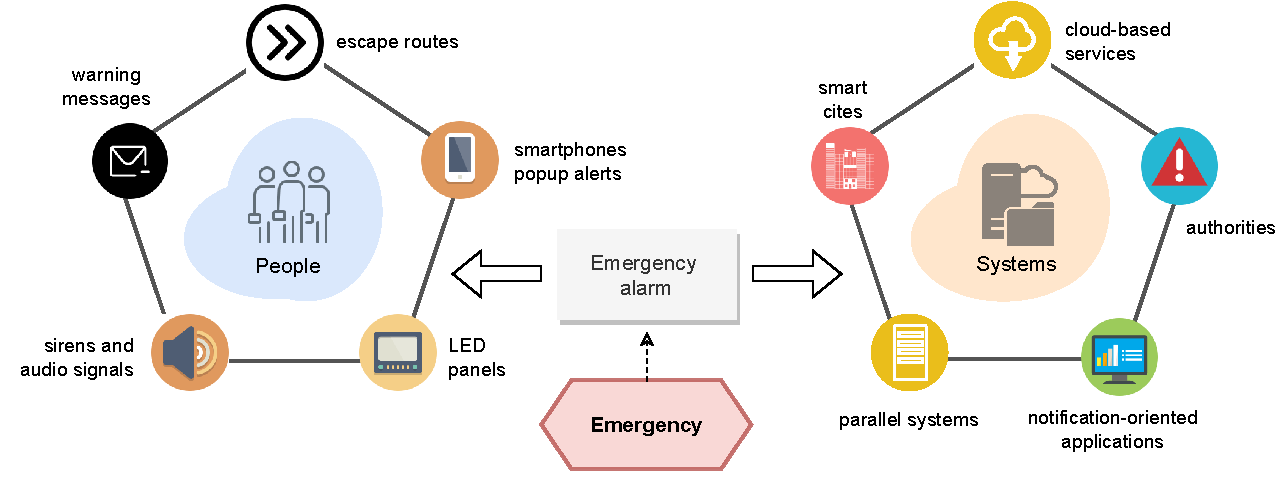
\includegraphics[scale=0.75]{Chapters/1-Survey/images/notifications.pdf}
\caption{Transmitting emergency alarms to different targets in a city.}
\label{Fig:notifications}
\end{figure*}

%%%
\subsection {Alerting affected people}

Directly alerting people has been a major concern when avoiding disasters in cities even before the age of computers, with the implementation of mechanisms to warn all or part of the inhabitants about something potentially dangerous. For example, bells and sirens have been adopted as an affordable and effective way to alert many people in a considerable extensive radius \cite{socialmedia5,citiesemergencies1}. However, notifications can also provide relevant information about the type of an emergency and its intensity, as well as information to guide people to move toward a safer place \cite{emergenciesmetric2}. Additionally, when considering notification strategies, safety plans have been also employed in many localities, with people being previously trained about the procedures to be taken after being alerted about an emergency \cite{quakeculture,citiesdisasters2}. Whatever the case, alerting affected people is a major issue of emergencies management systems, with different particularities to be considered. 

An alerting service is not simply the transmission of emergency alarms. When a person is in the core area of an emergency, she/he will need to receive a very quick and clear emergency alarm since the inflicted damages/injuries might be high. However, people in the neighborhood also need to be alerted, even in a different way. For example, people inside a room where a fire starts will need a more straight alert (e.g. emergency lights in the shape of an arrow pointing to the closest evacuation route), while people in other rooms in the same building may receive notifications in their smartphones indicating how they must orderly exit the building. 

Concerning modern alerting systems, particularly solutions employing IoT technologies, different strategies have been adopted to perform \textit{in loco} notifications. The idea is to alert about emergencies as soon as they are detected in an area, usually employing the same hardware processing units. The work in \cite{iotFire3} monitors fire sources inside a building and alerts people using a LED display to present a safe escape route. In \cite{alertdam1}, sensors are installed over a tailing dam to monitor the flow of debris after an accident, which will trigger flashing lights and sirens along the way to alert people. Since a city may be in the pathway of such flow of debris, this type of emergencies management system may have a deep impact on urban areas. In \cite{iotFire5}, smart exit signs are used to guide people during a fire emergency, changing the displayed information on real-time to update evacuation information. In all these cases, people do not need a gadget or tool to receive notifications, relying on the existing alerting hardware infrastructure. 

Alerting approaches can also directly target people exploiting other resources. In Poland, for example, the Government Centre for Security (GCS) alerts residents about disasters that may threaten their lives \cite{notification2}. After receiving emergency alarms, the GCS sends a notification to mobile network operators, so they can forward the notification to the residents' phones in the threatened area without requiring previous subscription to the service. In a similar perspective, the MyShake platform \cite{iotEarthquake4} considers different sources of data to perform Earthquake Early Warning (EEW), sending notifications to the smartphones of the inhabitants in a potentially affected area. Still considering earthquakes, the work in \cite{notification1} also proposes an EEW system called ShakeAlert that makes use of several seismologic sensors to detect earthquakes as soon as they begin. If some thresholds are exceeded, the system sends notifications to smartphones containing complementary information about the detected earthquake such as origin time, location, magnitude, and extension. 

Although the alerting method should be ubiquitous and quick enough to avoid as much losses as possible, some approaches require manual subscription to a stakeholder. The work in \cite{notification3} presents an early warning system for landslides in Chittagong, Bangladesh. That system makes use of a landslide factor map that describes the risk of landslide in every region of interest. Combining the factor map with weather forecast, the system calculates a risk of landsliding depending on the amount of rainfall that was predicted by the forecasting service. With this information, the early warning system sends e-mail notifications to subscribed stakeholders within 5 days in advance.

Usually, emergencies have been alerted by sirens and other types of audible and visible notifications in the cities. As technology advances and IoT-based devices get cheaper, new methods of alerting have arisen. In the majority of the surveyed works about emergencies alerting targeted at people, mobile messaging was an effective and affordable option, mostly SMS \cite{notification2,notification1,notification4,notification5, notification6} and even audio calls \cite{notification5}. This trend takes advance of the fact that almost every person has a mobile phone on her/his pocket during all day. In fact, it is expected that cellular networks and mobile apps will be of great importance for the development of more efficient emergencies management systems, assuring emergency alerting to many people at low cost. 

%%%
\subsection{Alerting parallel emergency systems}

The direct alerting procedures have the primordial objective of quickly warning people in order to avoid injuries and death. Although this is very reasonable in many cases, the development of more complex emergencies management systems has led to the adoption of modular architectures that separate the services of emergencies detection and alarms notification, which might be provided in a combined or separate way. In the later, alarms are delivered to any requesting system to be further processed, either indirectly forwarding the received alarms to affected people or retransmitting them to other systems.

An important element when delivering generic emergency alarms to other systems is the way data will be processed and formatted. In \cite{emergenciesmetric2,emergenciesmetric3}, emergency alarms are transmitted as JSON (JavaScript Object Notation) messages, organizing metadata in groups of significance. JSON is also adopted in a similar way in \cite{emergenciesmetric5}. For the work in \cite{emergenciesxml}, emergencies scenarios are described in XML (Extensible Markup Language) in a conceptual model for smart cities, which could be structured to represent emergency alarms. The XML formatting standard is also exploited in \cite{emergenciesxml2}, which defines a group of ten-tuple metadata for sensed data that can be easily consulted by other applications to identify emergencies. An extension of XML called CAP (Common Alert Protocol) can also be used to transfer emergency alarms between different systems, as in \cite{notification1}. Actually, the advantage of using formatting standards based on description languages such as JSON and XML is the standardization when describing alarms, allowing easy interaction between systems. Additionally, such languages are based on a flexibility principle when defining the formatting of a group of information, which is highly desired when implementing more complex emergencies management systems.

Other important implementation issue when transmitting generic alarms is the employed transmission paradigm. When considering previous works concerned with emergencies notification, we identified two main transmission paradigms, which are described as follows:

\begin{itemize}
    \item Subscription: When parallel systems want to be notified about emergency alarms, a subscription procedure is taken to register the requesting application. After that, alarms will be synchronously transmitted to all subscribed systems, which will process the received alarms in any possible way. For such transmission paradigm, protocols such as MQTT fit well, as proposed in \cite{emergenciesmetric2,emergenciesmetric3}. For those works, Emergencies Alarm Clients (EAC) subscribe to a MQTT broker to receive generic alarms in real-time. MQTT can also be used to deliver a particular type of emergency alarm, as in \cite{iotFire3,iotmqtt} for fire emergencies. Actually, many solutions based on MQTT have being recently implemented due to the flexibility and easy of use of this subscribe-publish architecture, which can operate over any network protocols. In this sense, many solutions have relied on ZigBee and LoraWAN protocols to assure a wireless transmission infrastructure, with MQTT delivering the emergencies alarms \cite{iotFire3,lora2,iotmqtt2}, assuring low energy consumption and possibly ad hoc transmissions for the considered system;
    
    \item On demand: Some approaches will not require the previous subscription of parallel systems to receive emergency alarms. In such cases, alarms and events-related data are made available in a way that it can be asynchronously accessed. In \cite{emergenciesmetric5}, alarms are saved in a web server to be consulted. In \cite{iotgadget1}, the RESTful architecture is exploited to create web services that provide data about emergency alarms. For \cite{emergenciesxml2}, 
    XML alarms are stored in a NoSQL database do be accessed by any requesting application. In the context of intelligent vehicle systems, the work in \cite{citiesvehicles3} broadcasts warning messages to vehicles in the area where accidents are detected. For such solutions, the nonexistence of a previous subscription process may reduce their overall complexity, although synchronous transmissions in a request-response notification paradigm may increase the time between the detection of an emergency and its proper notification.  
\end{itemize}

Alerting is indeed a vital service in modern emergencies management systems, which should be executed as soon as possible and reaching all affected elements in the area of an emergency. Actually, many approaches will also perform mitigation services in parallel, complementing the transmission of emergency alarms.
`

%%%%%%%%%%%%%%%%%%%%%%%%%%%%%%%%
%%%%%%%%%%%%%%%%%%%%%%
\section {Mitigating emergencies}
\label{sec6}

Although the alerting of people and external systems is a highly relevant objective itself, emergencies management solutions will also want to perform some actions to stop an emergency or even to reduce its negative impacts. Such actions are collectively grouped within the ``mitigation service'', which might ultimately have beneficial implications on the perceived quality of life in modern cities \cite{emergenciesmetric1,smartsensing3}.

Since there are different strategies when mitigating an emergency, the choosing of the best mitigation option concerning timeliness, cost and life preserving has been a major issue. For that, the most common approach has been to associate the nature of the detected emergency with a set of one or more mitigation actions. In this sense, for self-contained emergencies (Section \ref{sec2}), IoT-based solutions have been created to deeply integrate the detection and mitigation of a particular type of emergency, usually combining the operation of sensors and actuators \cite{smartcities2,PlatformsSC}. On the other hand, events-based emergencies have relied on proper definitions of metadata when issuing emergencies \cite{emergenciesmetric2,emergenciesxml2}, which will be leveraged when selecting the most adequate mitigation actions to be taken. In both cases, the nature of the related hazard is of paramount importance, demanding proper understanding of the dynamics of emergencies in urban areas \cite{citiesemergencies1,emergenciesgeneral1}. 

Therefore, emergencies can be mitigated in multiple ways, either directly within the area of incidence of the detected emergency, or even in a broader perspective comprising the dynamics of an entire city. Nevertheless, the evolution of research and development areas such as Internet of Things, Remote Sensing, Big Data and Artificial Intelligence, as well as the continuous maturation of the smart cities paradigm, have significantly changed the way emergencies can be mitigated in a city, improving the efficiency of mitigation approaches when saving lives and reducing properties damages \cite{smartcities1,smartcities2,smartcities3}. This integrated operation is, in fact, one of the promised advantages of smart cities, which puts emergencies mitigation as an inherent service of the cities of the future \cite{smartcities9}. 

Figure \ref{Fig:mitigation} presents an example of how a single emergency of fire can be mitigated in multiple different ways, either locally (triggering sprinklers and shutting down gas distribution in the area) or globally (requesting rescue teams and preparing hospitals to receive victims).

\begin{figure}[ht]
\centering
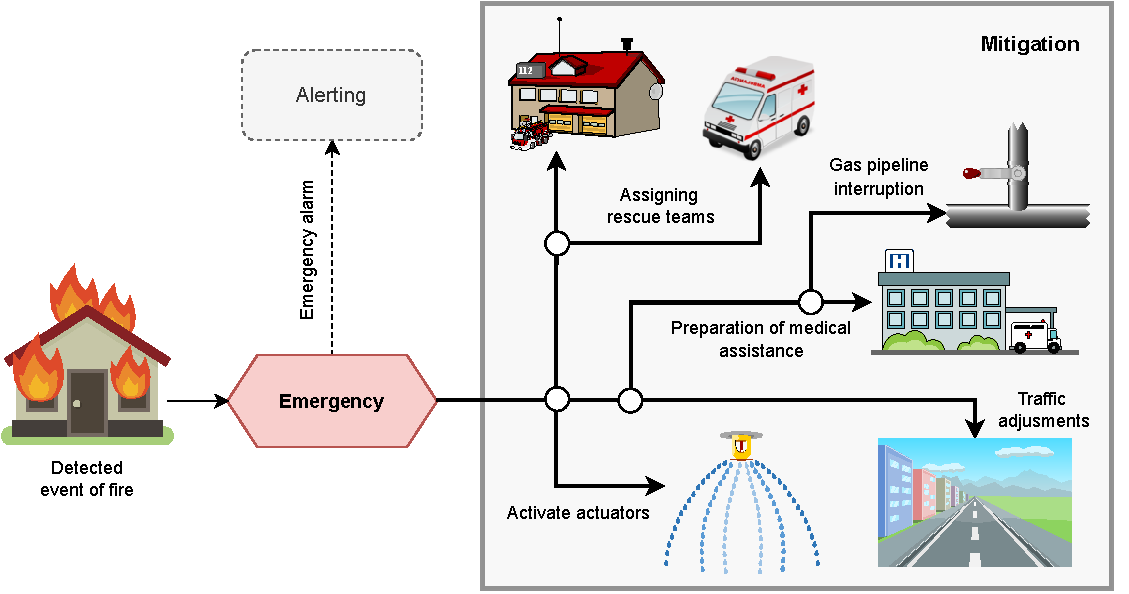
\includegraphics[scale=0.45]{Chapters/1-Survey/images/mitigation.pdf}
\caption{Mitigating a fire-related emergency. Mitigation services may have different objectives and areas of influence.}
\label{Fig:mitigation}
\end{figure}

When surveying mitigation approaches in the literature, it was noticed the adoption of two different strategies. The first strategy is based on direct actions on an emergency in order to cease its existence and to avoid that new emergencies are issued as a consequence of the initially detected emergency. Thus, in this strategy the target is the emergencies and how they can be handled. On the other hand, some works in the literature have been concerned with the impacts of the emergencies, relieving the negative outcomes that emergencies may have on people and properties. Both mitigation strategies have particular challenges in smart cities, being executed separately or in a parallel way, as discussed in next subsections. 

%%%%%%% 1
\subsection{Acting on emergencies}

When wondering about how an emergency can be mitigated in a city, one might say that the best approach is to fight the cause of that emergency. Actually, this is a very reasonable idea, since it has been the most usual approach when fighting emergencies in centuries \cite{fireevolution,firetemporaldata1}. With the advent of IoT technologies and sensor and actuator networks, such actions could be automatized in different ways, opening a new era of possibilities for emergencies mitigation in smart cities. 

Many automatized mitigation services have been proposed lately, employing different hardware components according to the type of emergencies to be mitigated. Actually, some proposed approaches are centered around one or more types of emergencies, which will dictate the type of actuators that will be more effective to mitigate a particular emergency. This fact can be seen in Table~\ref{Tab:mitigation}, which summarizes some works with these characteristics. 

\begin{table}
    \centering
    \caption{Some IoT-based approaches to directly act on emergencies in smart cities.}
    \label{Tab:mitigation}
    \begin{tabular}{|c|c|c|}
        
        \hline
        \textbf{Work} & \textbf{Emergency} & \textbf{Actions} \\
        
        \hline
        \citeauthor{mitigationAct1} \cite{mitigationAct1} & fire       & activate sprinklers \\

        \hline
        \citeauthor{iotEarthquake2} \cite{iotEarthquake2} & earthquake & turn off electricity, gas and water \\

        \hline
        \citeauthor{SultanMahmud2017} \cite{SultanMahmud2017} & fire   & turn off electricity, activate sprinklers \\

        \hline
        \citeauthor{iotFlood2} \cite{iotFlood2} & flood & open dam gates according to the water level \\
        
        \hline
        \citeauthor{mitigationAct3} \cite{mitigationAct3} & fire       & turn off electricity, release extinguishing gases \\

        \hline
        \citeauthor{mitigationAct4} \cite{mitigationAct4} & fire       & activate a water spray \\

        \hline
        \citeauthor{mitigationurban7} \cite{mitigationurban7} & fire       & dispatch drones do drop fire extinguishing balls \\

        \hline
        \citeauthor{mitigationAct6} \cite{mitigationAct6} & smoke       & activate smoke extraction fans \\

        \hline
        \citeauthor{mitigationAct7} \cite{mitigationAct7} & flood       & control watershed gates \\

    \end{tabular}
\end{table}

When acting on emergencies exploiting sensors and actuators, some interesting considerations can be taken. While works like \cite{SultanMahmud2017} and \cite{mitigationAct1} are intended to cease the cause of an emergency, directly facing the original hazard, the work in \cite{iotEarthquake2} can not avoid the issued emergency, but it can prevent the issuing of new emergencies derived from the original one. The same is true when adjusting traffic lights after an accident in order to avoid additional accidents \cite{mitigationITS1,rego2018software}. In all these cases, although the outcomes may be different, the employed approach will directly act on the issued emergencies.

Other important remark is about the level of automation in the implemented systems. In \cite{iotFlood2}, for example, sensors are used to monitor the level of dams, sending information to a data processing center. However, the decision of opening dam gates is made by personnel after analyzing the retrieved sensed data. Such human-assisted decisions are not rare since they may be valuable in some scenarios when the risks involved are too high \cite{humanAssisted1}.

%%%%%% 2
\subsection{Relieving emergencies}

The mitigation strategy for a group of approaches will be to relieve the impact that emergencies may have on people and the infrastructure of a city, reducing injuries, deaths and economical losses as good as possible. For that, an integrated perspective of a city is usually required, since such relief will depend on other services provided in a smart city context. As an example, while a mitigation service dedicated to act on a fire will try to extinguish it, a relieving strategy will contact an external system responsible for rescuing and firefighting in order to request the dispatching of ambulances and fire trucks toward the affected area. With the maturation of smart cities, more integrated solutions have emerged, promising more efficient support to emergency situations. 

When an emergency is detected in an area, the city may respond to facilitate the arrival of rescue teams and eventual supplies. Actually, fast arrival of rescue teams are critical during an emergency \cite{mitigationurban3}, which have fostered important research developments in this area. In \cite{mitigationurban1}, a logistics distribution approach is proposed to create a fast supply network toward affected areas, which may be created to last for longer than the expected duration of an emergency (e.g. when there is a perception that the emergency is turning into a disaster). Such approach, which comprises fuzzy-based decisions in a macro designing of a city, would be valuable before the dispatching of emergency vehicles such as ambulance and fire trucks, adjusting routes and potential relief areas. Similarly, the work in \cite{mitigationurban3} proposes a large-scale solution to support the mitigation of emergencies during a flood situation, specially focused in the accessibility of response teams. Since surface water and fluvial flooding may delay response teams during an emergency, multiple types of data in a city are considered to define optimal routing maps that should be taken by rescue teams in such conditions.

In several situations, first responder vehicles such as ambulances, fire trucks and police cars need to get to the emergency area as soon as possible. Since traffic can be jammed in large cities, some authors have proposed traffic management and signaling solutions in emergency situations. The work in \cite{mitigationurban4} is aimed at reducing the travel time of emergency vehicles during a mitigation process. In order to avoid wasted time due to red light signals, the authors proposed Arduino managed traffic lights. This way, the lights on the streets are managed by Arduino boards connected to the Internet that can receive commands from an Android application used by an emergency vehicle co-driver. That app can then be used to turn lights green in a way that the total travel time is reduced. However, while the work in \cite{mitigationurban4} requires manual intervention using an app, the authors of \cite{mitigationurban5} developed a semi-automatized approach that takes into consideration the current traffic in the city and also sets different priorities for emergency vehicles. A Central Traffic Controller (CTC) assigns movement priorities after gathering metadata of the issued emergencies, sending the routes to each emergency vehicle considering the current traffic conditions. With a GPS device in the vehicles, the CTC can get their position in real-time and then manipulate traffic lights directly. In a more automatized way, the work in \cite{rego2018software} divides a smart city into clusters comprised with smart traffic lights and electronic signaling. Once an emergency is detected, the system sends a message through the defined network asking for resources and informing the smart lights and signals how to operate to modify the traffic accordingly. When the emergency finishes, the system sends another message informing the lights and signals to resume their normal operations. 

Macro perceptions of traffic in a city are highly desired although the implemented solutions may become too complex. As an example, authors in \cite{s150614370} proposed a smart signaling system to inform users (citizens, drivers, etc.) of emergency situations. A system of connected sensors monitors the environment inside a tunnel and detects a fire situation, allowing the determination of the best exits according to the position of the fire source and smoke conditions. Then, smart signals are settled accordingly, directing the users to a safe exit.

Another problem related to emergency vehicles is the (automatic) assigning of rescue teams according to the type of the detected emergencies and their metadata. The work in \cite{costa2020automatic} proposes an emergency vehicles assignment algorithm according to the issued emergencies, selecting the most appropriate vehicles in a city that is experiencing multiple concurrent emergencies in different areas. In that work, the expected negative impact of each current emergency is assessed, being combined with the distance from the available emergency vehicles to the area of incidence of each emergency. The combined result of these parameters is then used to assign the most effective (and potentially closer) emergency vehicles. For the work in \cite{mitigationurban2}, sensed data are transmitted to a central unit to be processed along with other data. Then, issued emergencies are coordinately answered by mitigation actions, with the assignment of polices, firefighters or medical staffs teams according to the type of the issued emergencies. 

Relieving mitigation actions can also come from the sky. In \cite{emergencyRescue3}, camera-enabled drones are expected to support in rescue operations, identifying the number and the locations of victims in a building. For the work in \cite{mitigationurban6}, drones equipped with cameras are also considered to support rescue teams when identifying victims. In \cite{mitigationAct5}, drones are used to ``mark'' critical areas that need assistance during an emergency. In all these cases, drones are an important supportive resource, but they can also be used in different ways. In \cite{mitigationurban8}, drones are dispatched as a first response to an emergency call in order to provide initial information for the victims. Actually, when adopting microphones or even LEDs, drones can be a very fast response resource during emergencies, reaching areas that vehicles can not go. In fact, this perspective could be seen during the COVID-19 pandemic, with drones supporting social distancing measures \cite{dronecovid1} and sanitation \cite{dronecovid2}.  


%%% 7 %%%%%%%%%%%%%%%%%
%%%%%%%%%%%%%%%%%
\section{Open challenges and future directions}
\label{sec7}

The development of emergencies management systems have to deal with a lot of aspects related to the modelling of emergencies, the detection of emergencies, the transmission and displaying of warning messages, and the mitigation of emergencies in cities. These major concepts were surveyed and discussed in this article, giving important clues about important development issues and evolution trends in this complex area. However, although a comprehensive perception of the state-of-the-art in this complex subject has been provided in this article, some open challenges and future directions still need to be discussed, potentially supporting research efforts in the coming years.

\subsection{Technologies and development trends}

Roughly speaking, although technological aspects are highly relevant when implementing emergencies management systems in the era of internet of things, artificial intelligence and smart vehicles, this area is still evolving and new technological tools are constantly being developed. Actually, it is reasonable to expect that sensors-based systems and IoT devices will still drive the development of emergencies management systems, but their maturation will depend on new innovative ideas for the emerging challenges to be presented.

An important development trend is the utilization of low-power affordable miniaturized hardware to support in the detection, alerting, and mitigation of emergencies. Obviously, since each of these phases have particular challenges, as discussed in this article, such hardware is expected to be embraced in different ways. Notably, a recent trend has been to endow such hardware units with Machine Learning algorithms adapted to processing, memory, and energy constraints. This resulting TinyML paradigm should be one of the flagships for the new generation of emergencies management systems. 

The TinyML concept is highly suitable to the edge computing paradigm, which is another important development trend. Scattering the processing burden, more complex computations could be performed to allow the issuing of more complex aggregated emergencies. Since the smart cities environment is naturally prone to the execution of multiple parallel systems, the availability of multiple data source could be exploited by the computing on the edge, potentially leading to the quick execution of detection and response procedures. In our opinion, this is a promising development trend to be followed.

In parallel, recent works have started to develop soft sensors approaches to tackle the particular problems of smart cities \cite{softsensor,softsensor3}, virtually creating a layer of sensors with more complex (and abstract) data. Since soft sensors provide new types of data combing input data from sensors and other data sources, emergencies detection can directly benefit from this idea. Moreover, when TinyML is combined with the principle of soft sensors \cite{softsensor2}, more efficient EDUs could be designed at affordable prices. Future works in this area should then bring some breakthroughs for the development of emergencies management systems.

Besides the presented trends, other technological innovations that better support the development of cyber-physical systems in the context of smart cities should favor the maturation of emergencies management systems. We believe such hardware-software integration should be the cornerstone for new developments in this area.

%%
\subsection{Urban inequalities and smart solutions}

The urban sprawl since the initial industrial revolution has considerably changed the landscape of humankind, with large cities emerging in all continents and transforming our way of living. In this new environment, many inherent problems of large cities have driven research and development efforts in last decades, with challenges related to urban mobility, sanitation, pollution and energy efficiency encompassing major concerns. However, with the development of new technologies, the safety and well-being of the cities inhabitants have come to the table, which may significantly benefit the quality of life in urban areas.

Overall, smart cities have been promoted as a way to improve urban livability, becoming almost common sense that smarter cities are naturally better \cite{citylife}. However, since cities still have different social-economic organizations, many people may not have fair access to the cities resources, smart or not \cite{inequalities1}. Actually, some of the initially developed services in the smart cities trend were focused on efficient public lightning and traffic efficiency, which have been mostly implemented in richer areas of the cities that already had better urban infrastructure \cite{inequalities3}. A similar pattern can be perceived when considering the popular bike sharing service and the availability of greener public mobility alternatives \cite{smartcycling}. In fact, if not planned considering the general public interest, many smart cities solutions may become tools to increase social and economic inequalities. 

When coming to emergencies management systems, ``how'' has been a highly recurrent question that have driven most research efforts lately. However, ``where'' should also be a major concern, since the detection, alerting, and mitigation of emergencies should be provided regardless of socio-economic configurations and the pressures of the real state market. This concern should be more evident in this transition process from ``traditional'' cities to smart cities, mostly because the (initially) limited resources will eventually raise questions about which populations should be given priority in the allocation of such resources. 

It can be said that social vulnerability, population density, rescuing difficulties and potential of damage are some of the questions that should be answered before assuming that richer areas deserve better coverage by emergencies management systems \cite{emergenciesmetric1}. Therefore, considering the development patterns of large cities in the last centuries, fair access to smart cities services should remain an important challenge to be faced. 

%%%%%%%%%%%%%%%%%%%
\subsection{Infectious diseases as emergencies}

In 2020, a pandemic hit the entire globe within a relatively short amount of time. Due to fast well-connected transportation networks, the COVID-19 virus rapidly spread, leading to lockdowns and dramatically interrupting international trade routes and people circulation. In a sudden, our urban way of life facilitated the dissemination of the SARS-CoV-2 virus in a scale never seen before in the human history, raising a lot of questions about how the humankind can be prepared for the next pandemics.

The COVID-19 was the fist large pandemic that was faced in the era of smart cities. The state-of-the art in monitoring technologies, distributed databases and artificial intelligence algorithms could be put on service to track suspicious cases, to predict new infections and even to prepare hospitals to attend sick people. However, although the obtained results were significant when compared with the adopted measures in previous pandemics, the employed solutions were mostly punctual cases. Actually, with the maturation of smart cities and the consequent larger integration among systems, the full potential of health-centric services to predict, detect and isolate new infections might be achieved \cite{covidsmartcities2}.

Even after proper vaccination and the substantial reduction in the number of COVID-19 cases and deaths, it is reasonable to say that the post-pandemic world will be deeply impacted by the use of new technologies in public and private spaces. And this scenario, which will be naturally more prone for the adoption of distributed smart applications, will dictate how cities will evolve henceforth. As a result, smart cities initiatives are expected to be promoted more intensively in the coming years \cite{covidsmartcities6}.

Roughly speaking, the spread of a modern infectious disease can be perceived as a urban emergency \cite{covidsmartcities1}. This way, detection, alerting, and mitigation actions can be performed to handle an infectious disease outbreak or even a pandemic. Therefore, all previously discussed subjects and approaches could be leveraged to prevent or even to slow down a virus spreading. Particularly, some works have already focused on this matter, for example the work in \cite{twitter2} that uses the Twitter social media to detect an outbreak. Thermal cameras and image processing algorithms were also largely used during the COVID-19 pandemic to detect fever and potentially infected individuals \cite{covidsmartcities4}, and thus such technologies should still be used as standard tools. However, since a pandemic has a very wide perspective considering numerous aspects, comprising not only health assistance but also indirect services such as public transportation, the inherent integrated nature of smart city services might play an important role when detecting and even preventing next pandemics. For the evolving emergencies management systems, the next pandemic should always be a concern.

%%
\subsection{Smart cities development and integration}

A practical challenge for efficient emergencies management is the integration among the different systems within a smart city environment. Actually, most smart cities in the last decade have been developed as independent services with a well-defined set of objectives and input data. In this sense, cities around the world have seen some initiatives being developed and implemented as a practical service for the inhabitants \cite{citiestransforming,citiestransforming2}, but the actual integration among them is still in initial steps. The next generations of smart cities should then be devoted to such integration \cite{smartcities3}, which could not only incorporate the emergencies management service but also provide valuable data to support the detection, alerting, and mitigation of emergencies.

The smart city systems that are already being developed may present some opportunities for the evolution of emergencies management systems. The following are some of them \cite{citiestransforming}:

\begin{itemize}
    \item Smart healthcare: data provided by hospitals are valuable for different mitigation actions, specially when informing about the number of available ICU beds and the current configurations of medical assistance teams. During an emergency, such data provided by these parallel systems could indicate the best options when injured people need immediate assistance. When concerning ambulances, their number, location and current occupation is also relevant for mitigation actions: after an emergency is detected, the emergencies management system may send a request to the the smart healthcare system for the quick dispatching of ambulances to an affected area, taking all emergencies' metadata into account;
    
    \item Intelligent transportation systems: the way vehicles and public transportation will behave in a city may also be integrated to the management of emergencies. In this sense, not only traffic accidents detected by the traffic system may be forwarded to an emergencies management system, but also the traffic infrastructure may be adapted to deal with an ongoing emergency in a city. Actually, some recent works have already proposed some solutions in this area, but a deeper integration between both services may improve the achieved results. In this trend, we expected that Vehicular Networks (VANET) will become more popular and ubiquitous, with a higher potential for integration with other systems.

    \item Smart security: public security systems may also provide valuable data for the perception of emergencies, specially when considering urban hazards. Moreover, the existing infrastructure of cameras can be leveraged to enhance the detection capacity of emergencies management systems. In such integration, the monitoring resources in a city may be increased, even considering different objectives. As an additional trend, police vehicles may also be dispatched by a smart security system under request, which is in fact an important component of mitigation actions during an emergency;
    
    \item Smart environment monitoring: current monitoring systems that employ fixed sensors stations, drones and even remote sensing through satellites are becoming very common in many cities, providing not only a more accurate forecast but also alerting about potential dangerous weather conditions. Many of such systems already have emergencies detection capabilities, although they operate within a well-defined context. Hence, an integration could enhance the efficiency of emergencies management systems, while reducing the associated costs when already deployed sensors are concurrently used by both systems.
\end{itemize}

These and other potential integration among two or more smart city systems will have to deal with some integration challenges, demanding common interfaces. Since integration issues are also relevant in other smart cities contexts, some works have already addressed the development of smart cities systems that comply with defined standards \cite{snap4city,validation1}. In fact, validation of future proposed systems will be always an important design issue, with methodologies, evaluation labs, and supportive tools emerging to address this matter. Overall, we believe this will be one important development trend for emergencies management systems.

%%%%%%%%%%%%%%%%%
\section{Conclusions}
\label{conclusion}

For the development of more sustainable and resilient cities, emergencies should be treated as one of the main elements of the urban dynamics, potentially affecting multiple systems in a city environment. Actually, with most world population living in urban areas, with increasingly presence of large and mega cities, the negative impacts of emergencies and disasters have been more significant in the last decades. This scenario has fostered the adoption of different emergency-prone approaches in multiple contexts, but the challenges imposed by overcrowded cities will still demand more efficient solutions.

This article addressed technological issues of hardware, software, data, and networking related to emergencies management systems in urban scenarios. After the performed discussions, classifications and analyses, a comprehensive snapshot of this research area was obtained, potentially supporting a deeper understanding of its state-of-the-art.

As could be seen, smart cities will handle emergencies through detection, alerting, and mitigation services, which will be based on well-defined models and data formats. Although many solutions have been developed to address specific problems, as discussed in this article, it was perceived that a natural trend is to develop more integrated solutions, treating the city as a broader system with highly interconnected subsystems. This principle should be more often considered in future works. 

In general, detection, alerting, and mitigation are the pillars of emergencies management systems. Nevertheless, other important research subjects are also relevant and should be also considered when developing more efficient smart solutions for current and future emergencies, for example comprising research topics such as networking, security, energy efficiency, availability, among others. Since this whole research area is very active, with many new solutions still emerging in the coming years, very creative solutions integrating existing and new technologies should be proposed, bringing promising results.

% \bibliographystyle{unsrtnat}
% \bibliographystyle{abnt-alf}
% \bibliography{Chapters/1-Survey/references}

\printbibliography[heading=subbibliography]
\end{refsection}
    % --------------------------------------------------
% Capítulo 2: Posicionamento de EDUs
% --------------------------------------------------
\chapter{On the Positioning of Emergencies Detection Units Based on Geospatial Data of Urban Response Centres}\label{cap:posicionamento}

\begin{refsection}

\textbf{ABSTRACT}

Urban areas have been subject to emergency situations with different causes and sometimes dramatic consequences. With the advent of smart cities technologies, multi-emergency detection units could be conceived and implemented taking advantage of affordable sensing technologies and efficient decision algorithms, allowing quick and distributed detection of emergencies. However, a recurrent problem has been the positioning and further deployment of such detection units in a way that the particularities of each target city are properly considered. In this sense, this article proposes the processing of geospatial data about existing urban infrastructure associated with some critical response after an emergency is detected, selecting hospitals, police stations, fire departments, and metro stations, in the target city. These infrastructures are then exploited to define the novel concept of mitigation zones, which indirectly express the perceived level of urban resilience to emergencies. Then, four positioning algorithms are proposed to exploit the mitigation zones considering a defined set of available detection units for deployment. Since the proposed approach is valid for any city, provided that geospatial data is available, it could be largely adopted to support different smart city systems, potentially bringing significant results in this area.

\textbf{Keywords:} Smart cities, Sustainable and resilient cities, Emergency detection, Sensors positioning, Urban infrastructure.

\section{Introduction}\label{c2:introduction}

The development of more sustainable and resilient cities has been a major goal when the intense urbanisation process and the climatic changes are posed as dramatic challenges of our times \cite{surveycity3}. Lately, with the advent of new hardware, software, and communication technologies to support the development of more comprehensive cyber-physical systems \cite{surveycityPlatform1,surveycityPlatform2,surveycityPlatform3}, smart cities initiatives have emerged to bring innovative solutions to such complex challenges. In this context, some systems that are conceived to detect one or more types of urban emergencies and to act properly have gained attention, opening a new age for emergency and disaster management \cite{surveyEmergencies}. 

Any number and types of sensors can be attached to a Single-Board Computer (SBC) or a Microcontroller Unit (MCU) to create a multi-sensor Emergencies Detection Unit (EDU), which will be connected to some wired or wireless network to report when one or more critical situations are detected. The EDUs may be programmed to process data locally, defining on-the-edge approaches when detecting emergencies \cite{smartcitiesedge}, or they can rely on cloud-based architectures to distributively process data \cite{smarticiteshibrid}. Whatever the case, for a defined set of available EDUs to be deployed, a complex issue has been to find the best positions for them, which may consider not only technological issues but also the geospatial configurations of a city. Furthermore, since some positioning solutions have been tailored to specifically fit within the constraints of a particular city \cite{positions1,positions2}, a solution to this positioning challenge should also be adaptable enough to be efficiently applied to any city in the world. 

The problem of positioning sensor-based units has been usually approached by the understanding of the target city \cite{spatial2}. Generally speaking, a city is a very complex scenario comprised of people, its environment and existing infrastructure, which impact the way we live in urban areas. When taking the problem of emergencies management, comprising its detection, alerting and mitigation, the people-environment-infrastructure elements are highly related, intrinsically affecting each other. Particularly, the existing infrastructure associated with emergency mitigation, which is related to the actions taken after an emergency of any type is detected, can be leveraged as an important information when assessing the level of resilience of any city, potentially saving lives. As any emergency is being addressed following this concept, for any environmental adverse conditions, a comprehensive perception of urban emergency response is achieved. This multi-perspective reasoning can directly guide the deployment of EDUs for any city, in a more adaptive way, potentially improving the overall detection efficiency of the employed system.

For the EDUs positioning problem based on mitigation response centres in the form of existing urban infrastructure, we use geospatial data as the main reference when defining the proposed concept of Mitigation Zones (MZ). A MZ is defined based on the principle that when an emergency occurs, the city will try to act on that emergency in some way, either trying to cease the causes of the emergency or performing rescue and medical assistance operations for affected people. For example, mitigation actions may be associated with calling ambulances, dispatching fire trucks or diverting traffic flows. These actions, commonly referred as ``emergency mitigation'', may be performed by any emergency management system and the literature has presented many solutions for that \cite{surveyEmergencies,mitigation1,mitigation2}. The association of response centres with Mitigation Zones is the core element when guiding the positioning of EDUs in this article.

A mitigation response centre is defined as a Point of Interest (PoI), with hospitals, fire departments, police stations/posts, and metro stations (a type of urban mobility hub) as the list of PoIs to be considered. During an emergency, it is reasonable to expect that the distance between the affected area (emergency's spot) and the active set of PoIs in a city will be crucial when performing mitigation actions, since areas farther from response centres will be harder to be supported during an emergency, on average. This way, Mitigation Zones will be created according to the normalised distances to all PoIs in a city, automatically, according to a defined mathematical model. As the list of PoIs can be directly retrieved from open databases as OpenStreetMap, any city can be divided into multiple Mitigation Zones, making the proposed solution more flexible.

%%%
Four algorithms will be proposed to indicate the positions of the EDUs: Random, Balanced, Balanced+ and Restricted. For all proposed algorithms, it is considered the severity index of the zones as an input parameter, with a higher severity level zone (worse served by response centres concerning the computed normalised distances) proportionally receiving more EDUs than other mitigation zones closer to the considered list of PoIs. With that, a suggested position for each EDU can be achieved, which will further support the actual physical deployment of the nodes in a city. All proposed algorithms will be implemented and evaluated for the cities of Porto (Portugal) and Paris (France), with real data for the PoIs being considered. 

Figure \ref{fig:smartcity} presents a conceptual representation of how mitigation zones can be exploited to support the positioning of sensor nodes. The idea is that mitigation zones may be processed as data layers, each one comprising a particular perception of a target area according to the desired level of details being modelled.

\begin{figure}[htbp!]
  \centering
  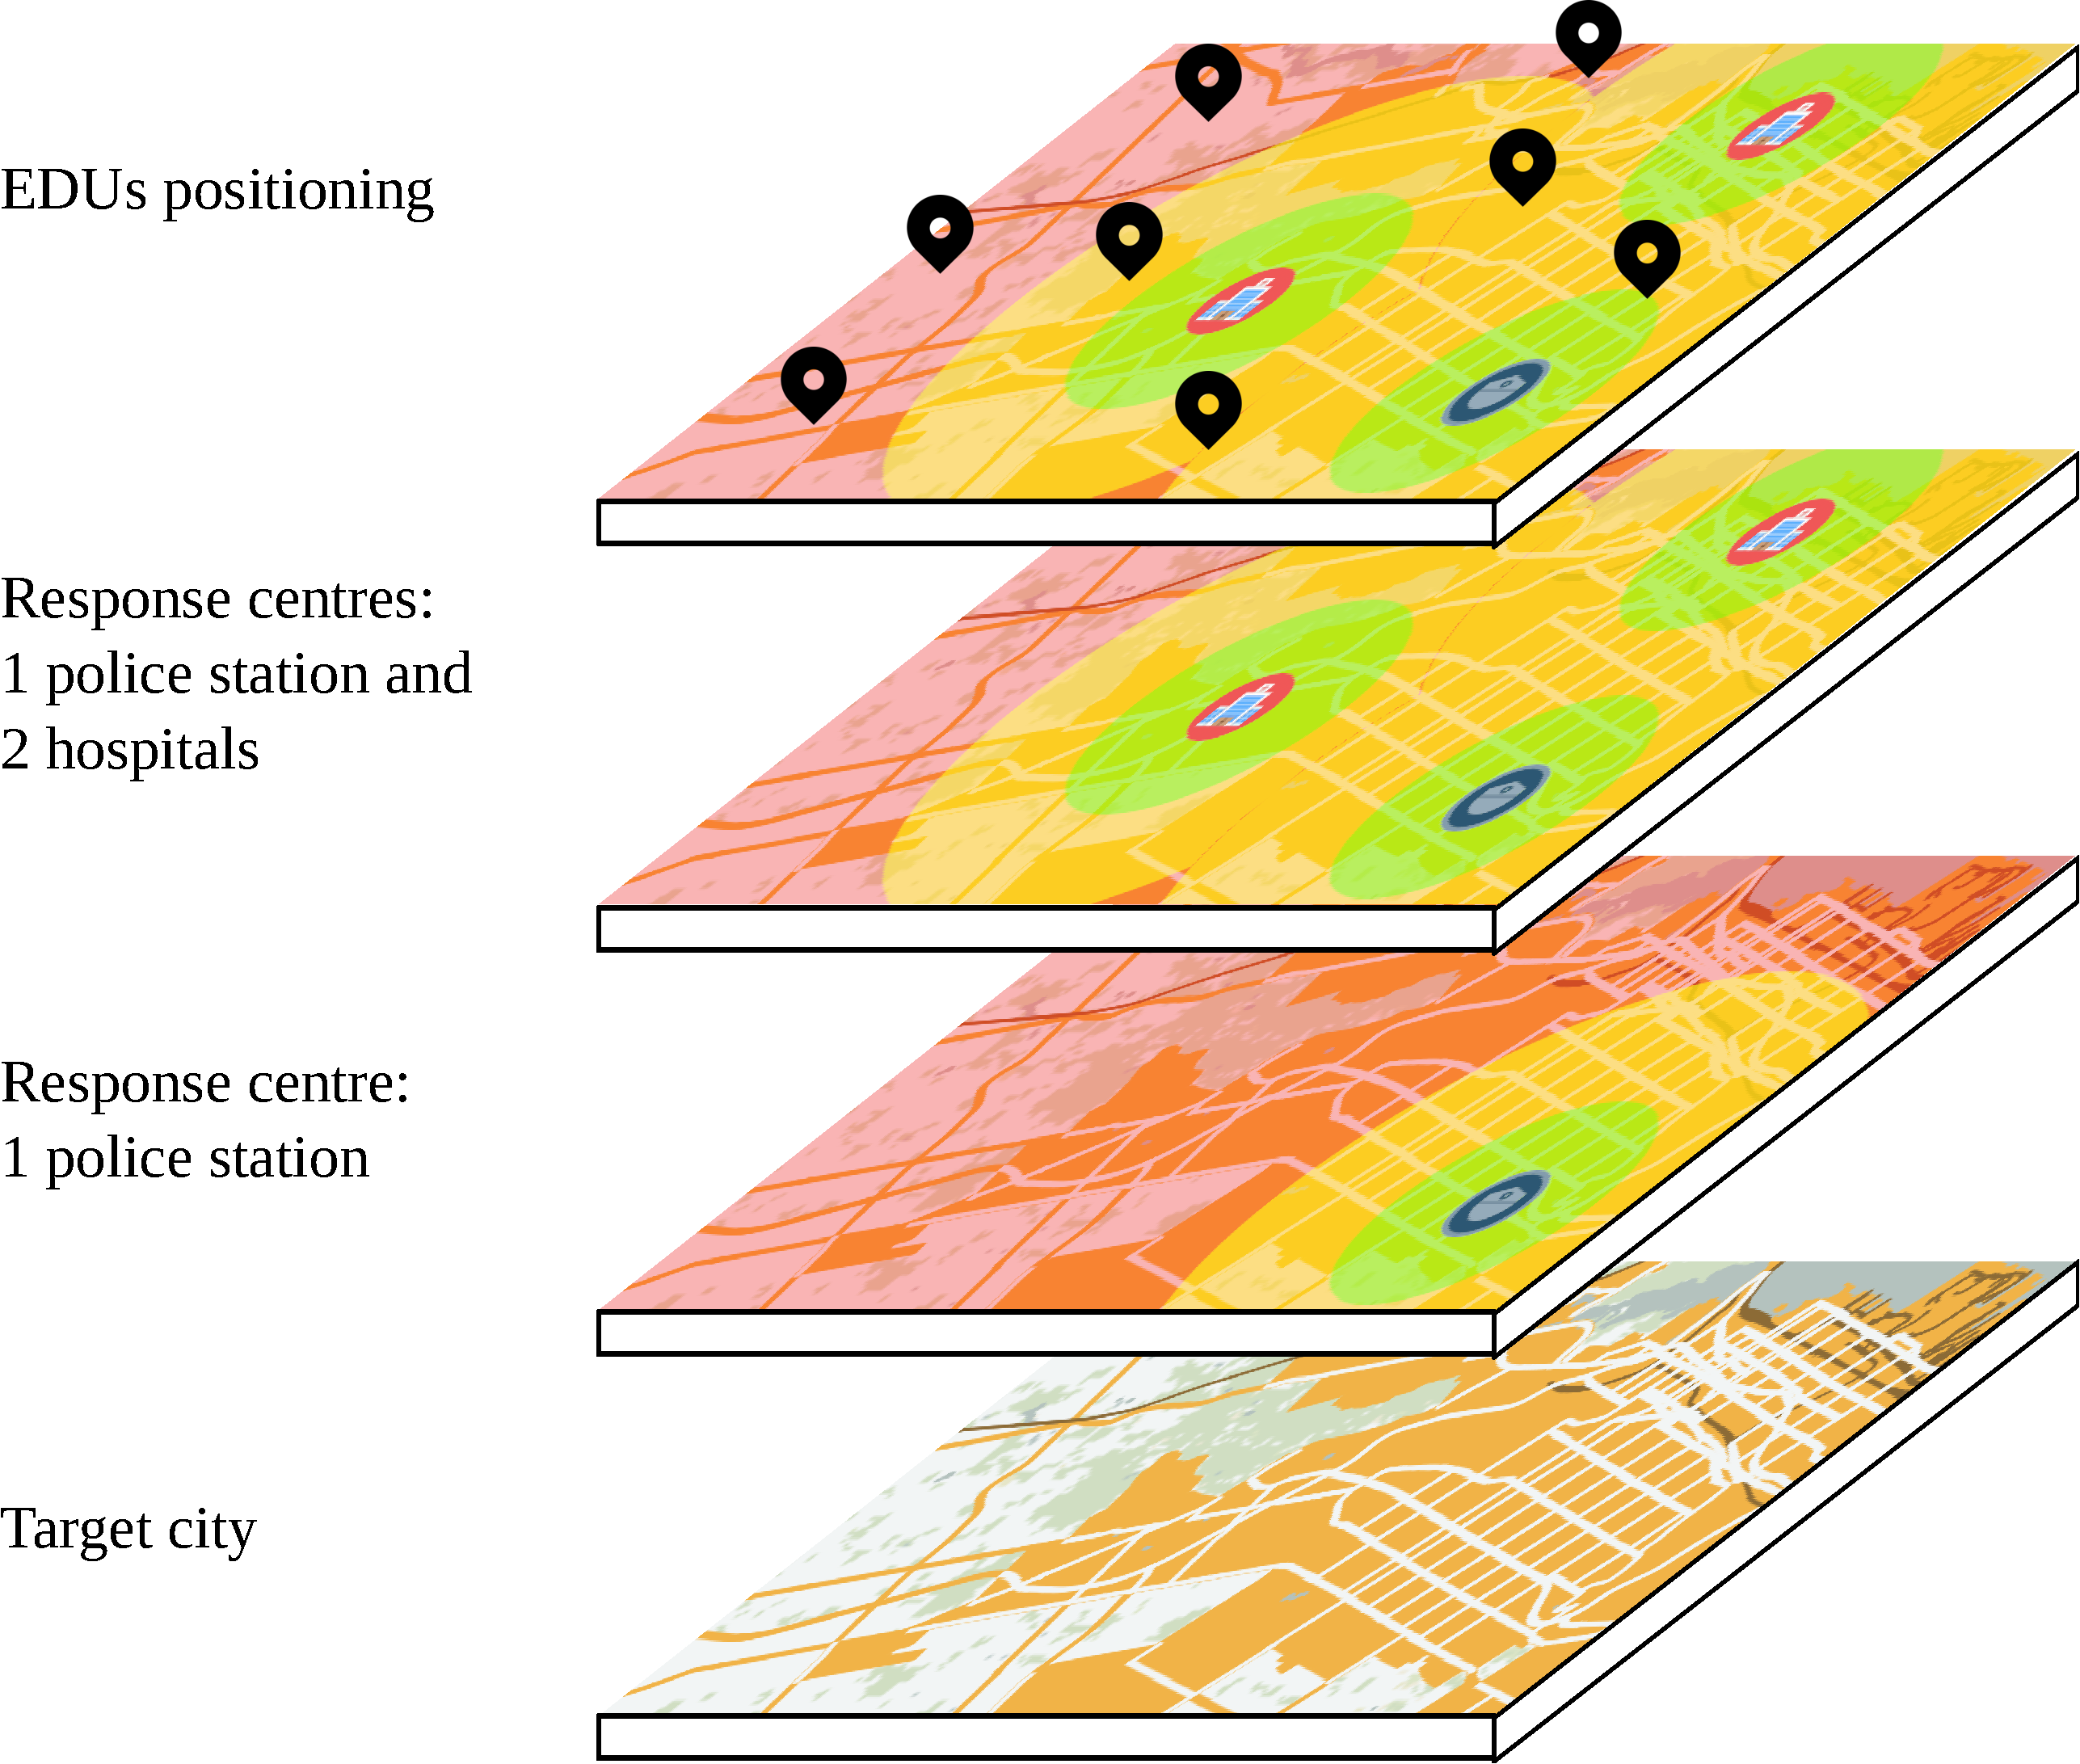
\includegraphics[width=0.7\linewidth]{Chapters/2-EDUs/images/map_layers.pdf}
  \caption{A conceptual representation for the definition of mitigation zones in a city.}\label{fig:smartcity}
\end{figure}

Therefore, considering the complexities of the presented challenges and the relevance of emergencies detection and mitigation for the creation of more sustainable and resilient cities, the contributions of this article are threefold, being described as follows:

\begin{itemize}
  \item Mathematical definitions for the concepts of Area of Influence, Mitigation Zone and Point of Interest, as well as the formulations to compute the severity indexes;
  \item The proposal of four EDUs positioning algorithms, with different expected results and costs;
  \item Experimental evaluations of EDUs positioning in two real cities, for different algorithms and input parameters.
\end{itemize}

The remainder of this article is organized as follows. Section \ref{S:2} presents related works in this area. The proposed mathematical model to compute mitigation zones and PoIs is described in Section \ref{S:3}. Section \ref{S:4} presents the four proposed EDUs positioning algorithms. Section \ref{S:5} brings experimental results and performance assessments. Final discussions and future directions are stated in Section \ref{S:6}. At last, conclusions and references are presented.

%%%%%%%%%%%%%%%%%%%%%%%%%%%%%%%%%%%%
\section{Related works}\label{S:2}

This work is concerned with algorithms to compute suggested deployment positions for multi-sensor Emergencies Detection Units (EDUs) in a city, taking as reference the existence of response centres when defining mitigation zones. Hence, related works addressing the use of geospatial data in smart cities, as well as the positioning of sensors within an urban scenario, were reviewed and discussed, supporting the developments in this article.

A central aspect of smart cities approaches is the retrieving, processing, and storage of large amounts of data, sometimes in a real-time basis \cite{surveycity1}. When managing urban emergencies, critical data that may be associated to an emergency have to be retrieved somehow and there are some solutions in the literature employing sensors, smartphones, social media, and open databases as data sources \cite{surveycity2,emergencies1}. Among such possibilities, sensors have been employed as affordable and highly flexible resources to retrieve scalar data as temperature, humidity, luminosity, CO\textsubscript{2} concentration, among many other variables, allowing a more distributed perception of how (and where) adverse conditions may happen in a city \cite{multiSensor,surveyEmergencies2}. Moreover, scalar sensors can also be combined with cameras and microphones to enhance the perception of the sensors' surroundings with multimedia data \cite{smartcitiescameras}. As a result, the literature has already presented many technological possibilities when implementing multi-sensor emergencies detection units, creating the foundations for more comprehensive emergencies management systems. However, EDUs positioning still remains a challenge when the particularities of each city has to be properly considered.

%% geospatial data
Smart cities are naturally benefited from the adoption of geospatial data in different scales \cite{sharingservices}. The use of longitude and latitude metadata associated to information extracted from an urban context may have many advantages, supporting more realistic perceptions about the different dynamics in a city \cite{surveygps}. For that, sensors-based units have been typically embedded with Global Positioning System (GPS) devices, while crowdsensing approaches and databases storing urban-related data have been usually tagged with GPS coordinates, allowing geolocation procedures for different purposes. Since many different solutions may apply, an important issue has been to properly select geospatial data sources for the defined problem scope.

Geospatial data may be central when pursuing the expected goals for a smart city application. In \cite{Fernandez_2015}, an approach was proposed to assess the urban vulnerability to flooding on parishes, specially considering old buildings in the city of Vila Nova de Gaia, Portugal. For that, information about population and buildings were considered when computing vulnerability levels, taking for that the positions of the parishes. For the work in \cite{Hondula_2015}, authors collected historical information of heat-related mortality, which are associated to data of existing urban infrastructure. In both works, socio-economic factors were associated to geospatial data, which has been a common approach in smart city initiatives.

Some works have been concerned with the processing of historical or real-time geospatial data from external databases \cite{realtimegis}, since such data could be exploited when making inferences. In \cite{uberdata1}, data from the Uber mobility service were exploited as an indirect indicator of the urban ``liveability'' of a city. In that work, the Estimated Time of Arrival (ETA) provided by an Uber API was correlated with some quality of life indicators, and thus such data could be used to create liveability maps for the target city. In \cite{openstreetmap2}, the OpenStreetMap open database was used to enhance the definition of local climate zones in cities, once more realistic urban data can be considered. In a different way, the work in \cite{googlemaps} exploited the Google Maps crowdsourcing tool to support the assessment of traffic conditions in a city.

In general, although previous works have highlighted the opportunities for geospatial data processing in smart cities when exploiting external databases, such works may be restricted by copyright issues and restrictions on data availability. This way, there is a trend to adopt open databases provided by governments and the inhabitants \cite{opendatabase1}, with living labs \cite{livinglab} and collaborative approaches \cite{cityspeed} having an important role in this trend. In this scenario, the OpenStreetMap open collaborative database has stood up, being considered as the main data source for many smart city approaches. 

%% positioning
The major objective of this article is to position emergencies detection units in a smart city, potentially assuring higher detection efficiency for a finite set of available units. To achieve that, geospatial data will be used to guide the positioning of EDUs, with open databases having an important role for this. Actually, some previous works have proposed different approaches to support the positioning of sensors in a city, influencing this work in different ways. In \cite{positioning1}, authors considered the roads map obtained from OpenStreetMap, as well as wireless connectivity issues, when positioning a set of sensors nodes, which resulted in the definition of deployment graphs. In that work, the transmission range was considered as an important input parameter for the placement of the nodes. In \cite{positions2}, some fixed multi-sensor units were used to complement data retrieved by a crowdsensing approach, with the actual positions of those fixed units being determined by experts in the target city of Porto, Portugal. Particularly, the defined positions of the units in that work took as reference the traffic, parking, residential, and touristic characteristics of the areas in the considered city. In a different way, authors in \cite{positioning3} considered the transmission range and the position of multiple sinks when positioning sensor nodes, without particular regard to the actual infrastructure and geographical characteristics of a city. These works are examples of how different geospatial data can be leveraged when positioning sensor nodes.  

At this point, it is important to note that geospatial data can be retrieved from different sources, with particular challenges to be handled. In some cases, data can be retrieved from social media \cite{twitterGeospatialSensors}, once latitude and longitude coordinates can be associated to public online posts. Additionally, crowdsensing applications can be used to support sensors deployment when positions of the contributing sources can be properly known \cite{positioning5}. In this article, OpenStreetMap is exploited to provide data about the roads and streets, as well as data of response centres within the considered urban area. Although different types of response centres could be considered, since the proposed mathematical model is flexible to encompass any type of Point of Interest, the performed experiments were concerned with hospitals, fire departments, police stations/posts, and mobility hubs (metro stations), which are very common in modern cities. 

%% Table
Table \ref{Table:related} summarises previous works in the literature, highlighting the employed source of geospatial data. 

\begin{table}
  \centering
  \caption{Some works exploiting geospatial data to support sensors positioning and deployment.}
  \label{Table:related}
  \resizebox{\textwidth}{!}{
  \begin{tabular}{c|c|c|c}
    \textbf{Work} & \textbf{Data source} & \textbf{City} & \textbf{Objective} \\ 
    \hline
    \cite{positioning1}  &  OpenStreetMap & many, Turkey & Roads monitoring\\ 
    \hline
    \cite{positions2}  & Experts in the target city & Porto, Portugal & City livinglab \\ 
    \hline
    \cite{positioning3} & Simplified geographical area & New York, USA & Generic sensing \\ 
    \hline
    \cite{twitterGeospatialSensors} & Social media & New York, USA & Sensors calibration \\ 
    \hline
    \cite{positioning4} & Group of existing buildings & Santiago, Chile & Monitoring of particulate matter \\ 
    \hline
    \cite{positioning5} &  OpenStreetMap & Seoul, South Korea & Air quality monitoring \\ 
  \end{tabular}
  }
\end{table}

%%%%%%%%%%%%%%%%%%%%%%%%%%%%%%%%%%%%%%%
\section {Fundamental concepts and mathematical model}\label{S:3}

The positioning of emergencies detection units in a target city will be guided by the presence of response centres, taking as reference their geospatial metadata and existing urban infrastructure. The response centres will be considered when defining mitigation zones, which is a proposed concept to mathematically support the positioning of any number of EDUs in any urban area. 

This article defines processing steps to be followed, both for the required mathematical modelling and for the positioning algorithms, as depicted in Figure \ref{Fig:figFluxograma}. The processing steps are presented along with the associated data sources and formats, highlighting the complete processing cycle of the proposed approach. The steps 1, 2 and 3 are described in this section.

\begin{figure}[htb!]
  \centering
  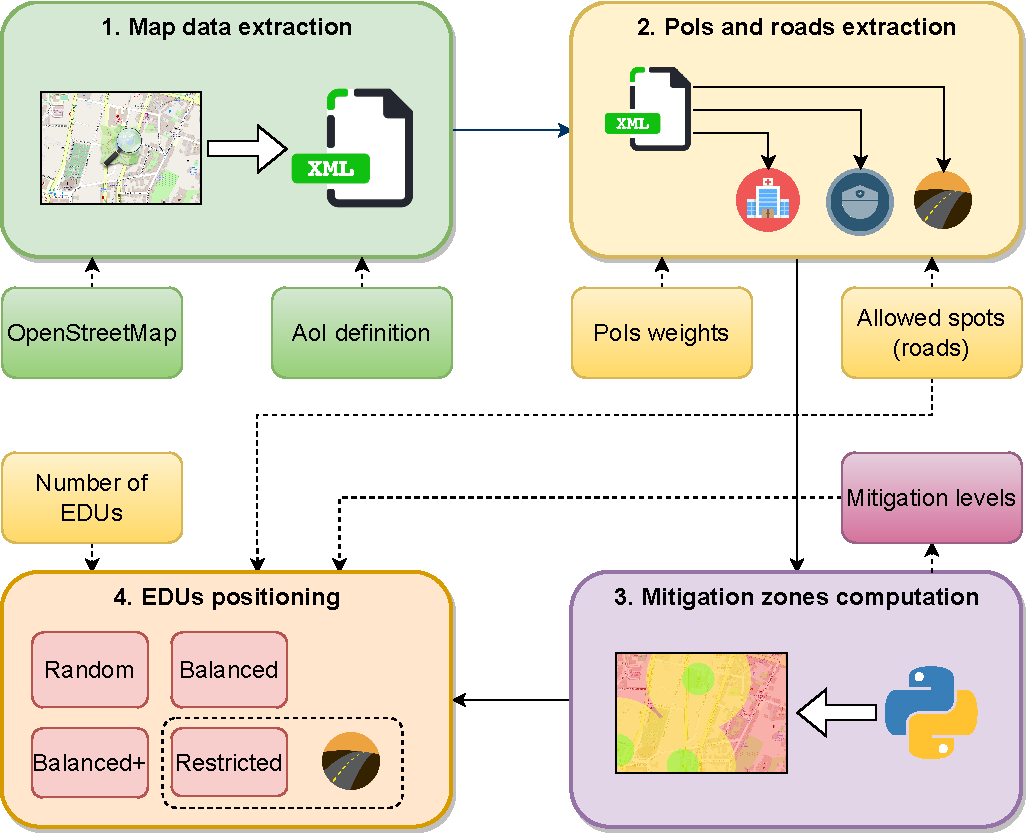
\includegraphics[width=0.85 \linewidth]{Chapters/2-EDUs/images/flowchart.drawio.pdf}
  \caption{The processing flow and data interactions in the proposed EDUs positioning approach.}\label{Fig:figFluxograma}
\end{figure}


%%
\subsection{OpenStreetMap and Points of Interest}

The availability of digital map databases to provide geospatial data about geographical elements on the ground has supported the development of different applications, with special attention to smart city projects \cite{spatial2,spatial1}. Among the available databases, OpenStreetMap (OSM) stands out as a crowdsourced geographic information database that is supported by collaborative work from volunteers worldwide \cite{openstreetmap}. This way, the maps are freely available for visualisation, query, download, and modification, being a powerful data source with no copyright restrictions. Additionally, as the users community can adapt the maps to quickly comply with changes in the real world, it is expected that the available information will be often reliable and up-to-date. Finally, a considerable number of flexible APIs are available for many programming languages, facilitating the retrieving and processing of geospatial data from this database.

In short, OSM defines a conceptual data model of the physical world, representing features on the ground like roads and buildings through the definition of ``nodes'', ``ways'', and ``relations''. Doing so, metadata are associated to the modelled elements, providing valuable data for different types of applications.

Among the available data in the OpenStreetMap database, response centres can be identified when searching queries are properly executed. As mentioned before in this article, the resilience of an area within a city will be associated to the presence (and distances) to response centres. Then, in a different way from previous works, we propose to compute the severity level of the mitigation zones (described latter in this section) based on the presence of such response centres, each one defined as a Point of Interest (PoI).

Actually, a city may have different types of response centres, which are some kind of urban infrastructure that may be associated to mitigation actions that would be triggered after the detection of an emergency \cite{surveyEmergencies}. In this context, for example, if an emergency happens near a hospital, there is a better chance to attend victims on time, and the same is true for a fire incident not far from firefighters. The challenge is then to identify such ``points'' and to extract their GPS coordinates, which can be retrieved from OpenStreetMap (or other geospatial database) using proper keywords. 

Hence, there will be $P$ points of interest, regardless of their types (e.g. hospitals, fire departments, bomb shelters, metro stations, helipads, police posts, etc), since we do not differentiate their roles when responding to a detected emergency, although we define four basics types of response centres for benchmark. Actually, a PoI is identified when it has some important role for emergency mitigation, either supporting direct response actions like dispatching ambulances or firetrucks, or supporting indirect actions like rescuing procedures and evacuation from affected areas.

Whatever is the defined list of points of interest, a PoI $p_j \in P$ will be associated to a weight function $f(p_j)$ to indicate how relevant is that infrastructure in a city (e.g. large hospitals may be more relevant than small ones), which is a subjective aspect of the proposed approach that allows some level of ``calibration'' to the particularities of a target city.

%
\subsection{Defining mitigation zones}

A Mitigation Zone (MZ) is the core element when guiding the positioning of EDUs. Overall, a city may have different numbers and configurations of MZ, depending on the considered parameters. For that, the first step when modelling mitigation zones is the definition of an Area of Influence (AoI), which is a geographical area that may sprawl beyond a city and comprise areas from different parts of a metropolitan area. Actually, since it is very common to have ``clusters'' of cities that create a continuous urban area, it is reasonable to consider a target AoI instead of a single city. 

An AoI will be modelled as a rectangle delimited by a top-left vertex at the ($A_x$,$A_y$) coordinates (latitude and longitude) and a bottom-right vertex at the ($B_x$,$B_y$) coordinates, which can be freely defined according to any constraint. This modelled rectangle can be perceived as a 2D plane, but Haversine distances will always be taken when needed (instead of Euclidean distances). 

The defined AoI will be divided into contiguous and disjointed square-shaped subareas referred as mitigation zones, each one with a known physical position and having the same dimensions (width/height of the defining square). Since there will be a set $Z$ of mitigation zones for an AoI, with each zone $z_i \in Z$, it is possible to define that a mitigation zone $z_i$ will be positioned at ($x(z_i)$,$y(z_i)$) coordinates, having a with of $l$ meters, and a mitigation level of $ML(z_i)$, for $0 < i \le |Z|$. The adoption of mitigation zones as squares can reduce the computational cost while still assuring reasonable accuracy, specially when small zones are defined. The total area of the resulting grid-like AoI can be computed by summing up the areas of all mitigation zones' squares.

The adopted approach of using configurable squares when defining the zones results in the fact that the value of $|Z|$ (the total number of mitigation zones) will directly depend on the chosen value for $l$. While larger zones are faster to compute, it is expected that the achieved accuracy will increase for shorter zones, giving flexibility when adopting the proposed approach. This way, the highest accuracy would be achieved when defining mitigation zones as single GPS coordinates, but the achieved outcome may not justify the additional computational cost in some cases. 

The value of $|Z|$ can be computed as presented in Equation \ref{eqZones}. The function $dist(pointA, pointB)$ computes the distance between the provided points using the Haversine formula, which returns more accurate distances when GPS coordinates are adopted. 

\begin{equation}
  \begin{split}
    \displaystyle Z_w &= \left\lfloor \frac{dist(A_x,B_x)}{l} \right\rfloor\\
    \displaystyle Z_h &= \left\lfloor \frac{dist(A_y,B_y)}{l} \right\rfloor\\
    \displaystyle \lvert Z \rvert &= Z_w \cdot Z_h\\
  \end{split}	
  \label{eqZones}
\end{equation}

Equation \ref{eqZonesPoints} defines the computing of the coordinates of any mitigation zone $z_i$, assuming \textit{mod} as the modulus of an integer division, and $i$ as an index within the $Z$ set.

\begin{equation}
  \begin{split}
    \displaystyle x(z_i) &= A_x + l \cdot (i\ mod\ Z_w)\\
    \displaystyle y(z_i) &= A_y + l \cdot \left(\left\lfloor \frac{i}{Z_w} \right\rfloor\right)\\
  \end{split}	
  \label{eqZonesPoints}
\end{equation}

Then, the centre point of the zones can be computed, defined as the $(x_c(z_i),y_c(z_i))$ coordinates, as presented in Equation \ref{eq1}. These coordinates are required when computing the mitigation levels of the zones.

\begin{equation}
  \begin{split}
    \displaystyle x_c(z_i) &= x(z_i) + \frac{l}{2}\\
    \displaystyle y_c(z_i) &= y(z_i) + \frac{l}{2}\\
  \end{split}	
  \label{eq1}
\end{equation}

At this point, the mitigation zones of an AoI are correctly modelled and ready to be processed. However, it is reasonable to incorporate the particularities of the modelled urban area, even though an AoI is mathematically defined as a rectangle. For example, the AoI rectangle may cover parts of a river or the sea that may not be regarded as areas for the deployment of EDUs. This way, mitigation zones may be removed from the set $Z$ during an additional processing step, using the limits of a city (or other parameter) as reference, although the set of considered rescue centres is not changed in this case. Actually, the OpenStreetMap allows the indication of the contours of any city, facilitating this process. Whatever the case, we expect that this additional processing step would not compromise the expected results of the proposed approach as a whole.

Figure ~\ref{Fig:figGrid} graphically presents the definition of mitigation zones.

\begin{figure}[htb!]
  \centering
  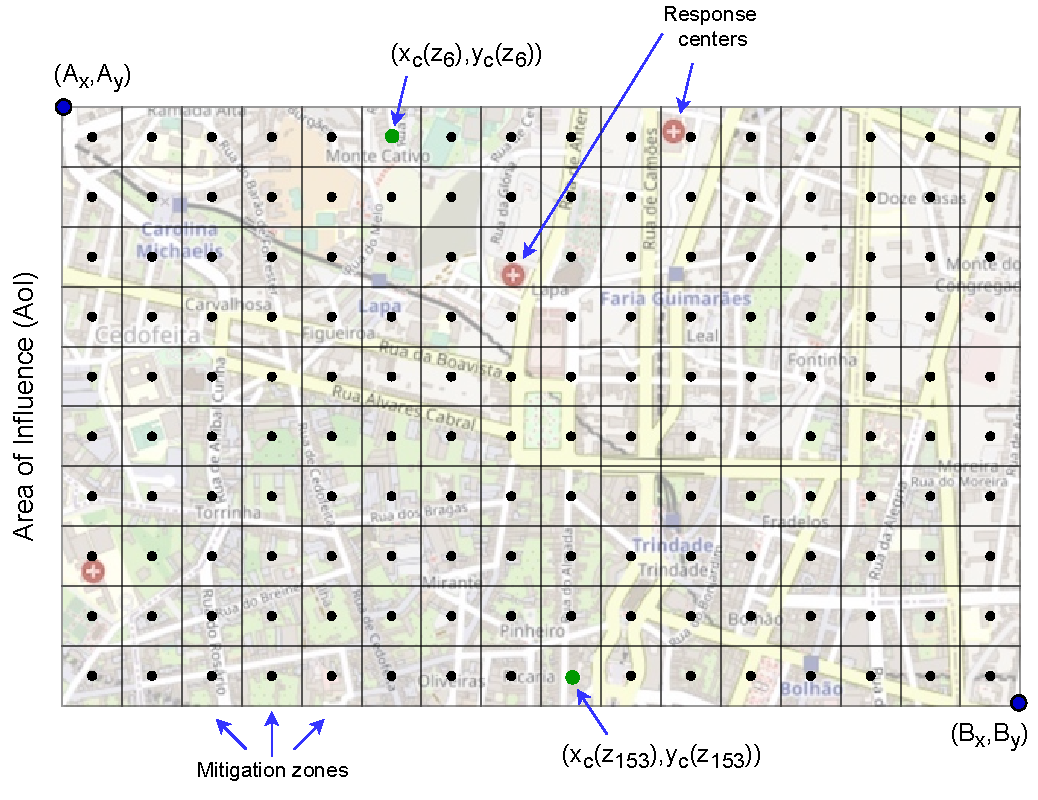
\includegraphics[width=0.77\linewidth]{Chapters/2-EDUs/images/MitigationZones.pdf}
  \caption{An example with 160 mitigation zones defined for an area of influence.}\label{Fig:figGrid}
\end{figure}

%
\subsection{Computing the mitigation levels}

Each mitigation zone will be tagged with a mitigation level, a numerical index within a previously defined range. The computation of the mitigation level of a zone ($ML(z_i)$) will happen after the definition of the list of PoIs and mitigation zones, being the last step before the positioning of the EDUs. 

The mitigation level of the zones will be computed based on an indirect relation between geographical areas and urban hazards and emergencies. Actually, to strongly associate hazards to the mitigation levels of zones may be too hard to achieve, demanding specific knowledge of a city or even taking other complementary data that may be not openly available. In a different way, we propose to consider the resilience to untreated emergencies according to the available urban infrastructure, which is easier to be mathematically processed in a more generic way \cite{emergencies1}. As discussed before, such resilience is indirectly accounted by taking the list of Points of Interest within the AoI.

Therefore, the higher the likeability of a region (and people) to recover from an emergency supported by existing PoIs, the higher is its resilience. This way, the balanced proximity of a zone $z_i$ to mitigation-related facilities (response centres) will indicate its mitigation level. As discussed before, different types of points of interest may be defined for an urban area, as long as their GPS coordinates are known.

Initially, it is performed the summing up of the squared distances from each zone to every PoI $p_j \in P$, multiplied by its weight factor $f(p_j)$. We adopt a weight factor to define the importance level of each PoI within an urban area, since some PoI may have higher importance during mitigation actions (e.g. larger hospitals or fire departments with better equipped trucks). Equation \ref{eq:risk_level} defines the performed computation in this processing step, for $E(z)$ as the combined risk perception of zone $z$ and $dist:Z,P~\to~\mathbb{R^+}$ as the distance function from a zone to a PoI.

\begin{equation}
  \label{eq:risk_level}
  E(z_i) = \cfrac{1}{\displaystyle\sum_{j = 1}^{\lvert P \rvert}\left(\cfrac{1}{dist^2(z_i, p_j)} \cdot f(p_j)\right)} 
\end{equation}

After computing the risk perceptions, the mitigation levels of each zone can be computed. This way, it is defined that $ML(z_i) \in M$, with $M$ as a set of ordered consecutive positive integers starting from $1$ until $|M|$: since the set $M$ is configurable, the value of $|M|$ will indicate how many different mitigation levels are being considered. Equation \ref{eq:risk_class} presents the computation of $ML(z_i)$, with $ML(z_i)~=~1$ as the lowest mitigation level and $ML(z_i)~=~|M|$ as the highest level. Additionally, $ML:Z \to \mathbb{N}$ is defined as the mitigation level classification function of a zone $z_i$, for $\widehat{E}$ as the normalisation of the risk perception function $E(z_i)$. 

\begin{equation}
  \label{eq:risk_class}
  ML(z_i) = M - \min\left(M - 1, \left| \left\lceil \ln{\widehat{E}(z_i)} \right\rceil \right| \right)
\end{equation}

As an important remark, the classification of each zone as being in one of the possible mitigation levels is relative to the region being considered. In other words, a zone is as risky as other zone with the same mitigation level if they belong to the same defined AoI, and thus it is meaningless to perform comparisons of zones if they are processed within different areas of influence. 

An additional consideration in Equation \ref{eq:risk_class} is that a natural logarithmic computation is performed when achieving the risk levels of the zones. In fact, different bases for the logarithm function could be adopted, with different final results for the zones, but it has been common in the literature to adopt natural logarithms (base $\mathrm{e}$) when computing classes and groups for different urban variables, particularly due to its mathematical properties \cite{log3,log4,log1,log2}.

Figure \ref{Fig:figGrid2} depicts a visual example of an AoI after computation of the mitigation levels. 

%\vspace{-3cm}
%\setlength{\textfloatsep}{0pt}

\begin{figure}[htbp!]
  \centering
  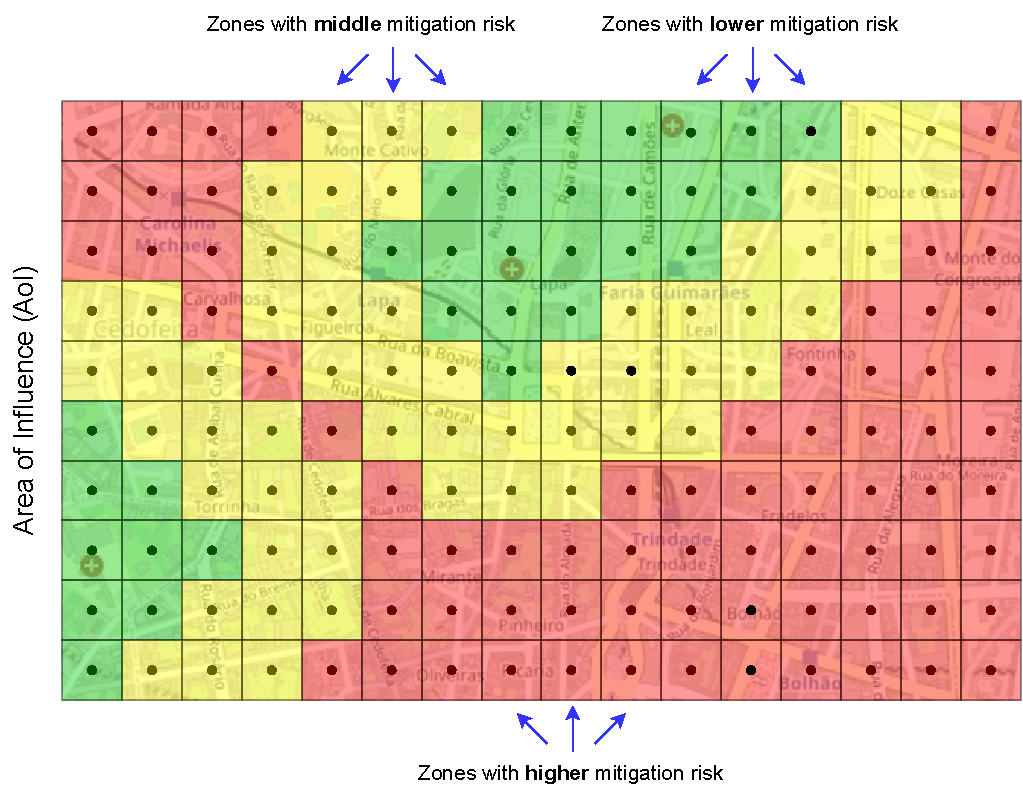
\includegraphics[width=0.77\linewidth]{Chapters/2-EDUs/images/MitigationZonesColors.pdf}
  \caption{An example of zones after computing the mitigation levels, for $|M|=3$ and 3 considered points of interest.}\label{Fig:figGrid2}
\end{figure}

In the example in Figure \ref{Fig:figGrid2}, $|M|=3$ and a grid of $16~\times~10$ mitigation zones is defined. Since we adopt a similar pattern of common heatmaps, it is defined that $ML(z_i)~=~1$ is green, $ML(z_i)~=~2$ is yellow, and $ML(z_i)~=~3$ is red, when plotting on a map for $|M|=3$.


%%%%%%%%%%%%%%%%%%%%%%%%%%%%%%%
\section{Proposed positioning algorithms}\label{S:4}

After the computation of the mitigation level ($ML$) of each zone within the defined AoI, the geospatial risk perception can be now mathematically computed. With this information, the step 4 of the flowchart depicted in Figure \ref{Fig:figFluxograma} can be executed. Actually, in this next step of the proposed approach, different algorithms might be applied, with different complexities and expected results. 

A total of four different EDUs positioning algorithms are proposed in this work. In general, the proposed algorithms have to compute how many EDUs will be allocated to each mitigation level in order to better monitor the zones and reduce the average impacts of emergencies. For that, since zones with higher $ML$ will be potentially harder to be assisted by emergency response actions due to their proportional distance to the existing PoIs, those zones should be better covered by EDUs in order to prioritise critical events detection in such less assisted areas. In other words, it is intended to prioritise zones with higher computed risk in order to achieve a better behaviour on average, proportionally better covering areas that would be worst affected by emergencies. Doing so, we expect to potentially achieve a fairer emergency-centred smart city service by not neglecting areas in a city that are already badly assisted by public services. The challenge is then how to distribute the selected EDUs for the mitigation levels, with different options available for that.

Whatever is the chosen strategy, the proposed algorithms do not compute the ideal number of EDUs required to cover the entire AoI. Instead, governmental entities and urban stakeholders must indicate the number of available EDUs for deployment, leaving the positioning decisions to the algorithms. This way, for the total number of EDUs defined as $U$, the number of EDUs in each zone is computed as defined in Equation \ref{eq:classes_distribution}.

\begin{equation}
  \label{eq:classes_distribution}
  \begin{split}
    \displaystyle n_m &= \frac{U}{\displaystyle\sum_{h = 1}^{|M|}\left(h \cdot a_h\right)} \cdot (m \cdot a_m)
  \end{split}
\end{equation}

Equation \ref{eq:classes_distribution} calculates the number $n_m$ of EDUs in each level $m$ in order to create a proportional distribution of sensing units, considering the total area $a_m$ of each level, prioritising zones with higher mitigation levels while restricting the total number of EDUs to $U$ units. After the computation of the number of EDUs in each mitigation level, an algorithm sets the position of every unit within the AoI. Depending on the chosen algorithm, the number of selected EDUs may vary around the value of $U$. That happens because the provided value for $U$ may not be suitable to fulfil the whole AoI according to a criteria defined by each algorithm.

Four proposed positioning algorithms are described in this section: \emph{Random}, \emph{Balanced}, \emph{Balanced+} and \emph{Restricted}. Each algorithm follows a particular positioning approach, presenting different computational costs. In a general sense, every proposed algorithm is an improvement of the former one, making the Restricted algorithm the more realistic and potentially most adequate for real-world scenarios.

\subsection{Optimising the coverage area}

For better detection of emergency events, the EDUs must cover the larger area possible inside the AoI. If there are enough units to be deployed in a way that every zone can be reached by at least one of them, we have a full coverage distribution, but this is not always the case. Our approach takes into consideration the fact that the EDUs are a limited resource and depending on the AoI size it will not be possible to have units enough to cover the whole area. This raises an optimisation problem, which is: given some restrictions, we must maximise the coverage area of the sensing units through a positioning schema. These considerations are stated as follows.

\begin{itemize}
  \item Restrictions:
  \begin{enumerate}
    \item Total number of EDUs ($U$);
    \item Number of EDUs per mitigation level ($n_m$).
  \end{enumerate}
  \item Goal: to maximise the overall coverage area of the AoI by the EDUs.
\end{itemize}

In this process, the EDUs must be distributed in an equidistant manner, spreading over the whole AoI as possible. The restrictions limit the number of EDUs in the whole AoI as also per mitigation level in order to obey the proportion distribution presented in this section. Thus, placing the EDUs in an equidistant manner will provide the best coverage solution as long as every EDU has the same sensing radius. Placing the EDUs too close to each other will create overlapping zones, reducing the coverage area. Such overlapping may happen in some situations depending on the area of the highest ML and the number of EDUs, but the equidistant positioning will always produce the scenario with less overlapping. In fact, the overlapping area of two sensing units can be obtained by calculating the area of two intersecting circumferences as shown in Equation~\ref{eq:overlapping_area}.

\begin{equation}
  I = r^2(\theta - \sin(\theta))
  \label{eq:overlapping_area}
\end{equation}

In order to maximise the coverage area, overlapping has to be minimised, and thus we have to minimise the value of $I$. Since $r$ is fixed, to minimise $I$ we must minimise $(\theta - \sin(\theta))$. The angle $\theta$ is the angle formed by the radius of any of the overlapping circumferences and the two intersection points as show in Figure~\ref{fig:circle_intersection}. This angle increases when the two circumferences get closer and decreases otherwise, thus, keeping the circumferences distant obviously reduces the overlapping area. Finally, placing the EDUs in an equidistant manner will avoid unnecessary overlapping and provide the maximum coverage possible, which guides the operation of the proposed algorithms.

\begin{figure}[htbp]
  \centering
  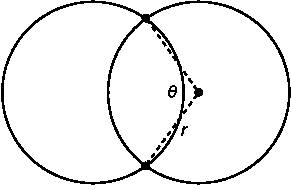
\includegraphics{Chapters/2-EDUs/images/circumferences_overlapping.pdf}
  \caption{The angle $\theta$ formed by the radius and the two intersection points.}\label{fig:circle_intersection}
\end{figure}

%%
\subsection {Random algorithm}

The first proposal for the EDUs follows a random positioning principle, according to the proportion ratio defined in Equation \ref{eq:classes_distribution}. The idea is that any position is valid for an EDU $z_i$ as long as the mitigation levels of the zones are considered to define deployment subsets. For example, assuming that $|M|=3$, there will 3 disjoint subsets of EDUs that may be positioned anywhere within the corresponding zone, since the combination of these 3 subsets results in the initial set of available EDUs.

The Random algorithm has the lowest computational cost, but it has no criteria for selecting the positions of the units. This way, it does not guarantee that every ``part'' of the AoI will be covered by an EDU. Actually, although it can be used to demonstrate the proportional distribution calculated in Equation \ref{eq:classes_distribution}, it is reasonable to say that this algorithm is not recommended for a real scenario of nodes deployment. 

The Random algorithm works as follows: after computing the number of EDUs per level, it randomly selects a position within the set of zones with that mitigation level for each of those EDUs. In this manner, it is possible to have several EDUs very close to each other, as well as some uncovered areas within the AoI, as defined in Algorithm \ref{alg:random}.

%%% Random algorithm
\begin{algorithm}[ht]
  \caption{Random positioning algorithm.}\label{alg:random}
  \begin{algorithmic}
    \REQUIRE $Z[] \gets$ the list of zones in each level, $M \gets$ number of levels, $N[] \gets$ number of EDUs needed in each level
    \ENSURE $pos[] \gets$ the list of zones that will get an EDU
    \FOR{$i$ from $1$ to $M$}
      \STATE $zones \gets random.choices(Z[i], k \gets N[i])$
      \STATE $pos[i].append(zones)$
    \ENDFOR
  \end{algorithmic}
\end{algorithm}


%%%
\subsection {Balanced algorithm}

After the definition of the mitigation zones, the Balanced algorithm calculates the EDUs coordinates within the AoI in a way that an uniform positioning distribution is achieved. This approach tries to eliminate the problems of the Random algorithm, avoiding uncovered areas and EDUs overlapping. In this sense, the Balanced algorithm calculates the coverage radius of the EDUs in each mitigation level in a way that the units are separated from each other in the same distance. The coverage radius is the distance that the units must be separated from each other in order to uniformly cover the zones with the same mitigation level. 

The Balanced algorithm computes the coverage radius in each level by dividing the total area of the zones with the same mitigation level by the number of EDUs in it, as presented in Algorithm \ref{alg:balanced}. 

%%% Balanced algorithm
\begin{algorithm}[ht!]
  \caption{Balanced positioning algorithm.}\label{alg:balanced}
  \begin{algorithmic}
    \REQUIRE $Z[] \gets$ the list of zones in each level, $M \gets$ number of levels, $N[] \gets$ number of EDUs needed in each level, $w, h \gets$ size of the AoI
    \ENSURE $pos[] \gets$ the list of zones that will get an EDU
    \FOR{$i$ from $1$ to $M$}
      \STATE $radius[i] \gets numpy.sqrt(Z[i] / N[i]) / 2$
      \STATE $step[i] \gets 2 * radius[i]$
    \ENDFOR
    \STATE $step_x \gets 0$
    \STATE $step_y \gets 0$
    \FOR{$y$ from $0$ to $h$}
      \STATE $step_y \gets step_y + 1$
      \FOR{$x$ from $0$ to $w$}
        \STATE $step_x \gets step_x + 1$
        \FOR{$i$ from $1$ to $M$}
          \IF{$step_x$ mod $step = 0$ \textbf{and} $step_y$ mod $step = 0$}
            \STATE $pos[i].append(zone(x, y))$
            \STATE $step_x \gets 0$
            \STATE $step_y \gets 0$
          \ENDIF
        \ENDFOR
      \ENDFOR
    \ENDFOR
  \end{algorithmic}
\end{algorithm}

This way, it is possible to determine how the units must be set apart to cover the whole area without overlapping or creating uncovered zones. After having the coverage radius, the algorithm sequentially position every EDU in an area, creating an uniform grid of multi-sensor units.

As an important remark, although this algorithm achieves an uniform positioning, it does not guarantee coverage around the levels' borders nor avoids overlapping (between neighbour zones) in these regions.

%%%%
\subsection {Balanced+ algorithm}

The Balanced+ algorithm improves the Balanced algorithm by guaranteeing that the units are positioned correctly even in the border zones, being an enhanced version of the later. In this approach, every time an EDU is positioned, the algorithm checks if its distance from the nearest unit obeys the coverage radius that was previously calculated. In this sense, there is no overlapping in border areas and there is no uncovered areas within the AoI.

The computational cost of this algorithm is much higher than the ordinary Balanced method because of the several checks that it performs when positioning each EDU. This proposed algorithm is presented in Algorithm \ref{alg:enhanced}.

%%% Enhanced algorithm
\begin{algorithm}[ht!]
  \caption{Balanced+ positioning algorithm.}\label{alg:enhanced}
  \begin{algorithmic}
    \REQUIRE $Z[] \gets$ the list of zones in each level, $M \gets$ number of levels, $N[] \gets$ number of EDUs needed in each level, $w, h \gets$ size of the AoI
    \ENSURE $pos[] \gets$ the list of zones that will get an EDU
    \FOR{$i$ from $1$ to $M$}
      \STATE $radius[i] \gets numpy.sqrt(Z[i] / N[i]) / 2$
    \ENDFOR
    \STATE $smallest\_radius \gets radius[M]$
    \STATE $highest\_radius \gets radius[1]$
    \STATE $minumum\_dist \gets 2 * highest\_radius$
    \STATE $x \gets 0$
    \STATE $y \gets 0$
    \WHILE{$y < h$}
      \WHILE{$x < w$}
        \IF{$dist(zone(x, y), nearest\_edu) \leq minimum\_dist$}
          \STATE $x \gets x + 1$
          \STATE break
        \ENDIF
        \STATE $pos[i].append(zone(x, y))$
        \STATE $x \gets x + 2 * smallest\_radius$
      \ENDWHILE
      \STATE $x \gets 0$
      \STATE $y \gets y + 1$
    \ENDWHILE
  \end{algorithmic}
\end{algorithm}

The Balanced+ algorithm works as follows: after calculating the number of EDUs per level, it performs the coverage radius computation in the same way of the Balanced algorithm. The difference between both approaches lies on the positioning step. The enhanced Balanced+ algorithm checks if there is any other unit in the proximity of each EDU, checking if it would ``fail'' the desired coverage radius distance. If there is any other unit too close to the EDU being positioned, the algorithm moves the EDU until it gets the correct distance from its neighbours. The other change in this algorithm is related to how it positions sensing units on the borders of different mitigation levels areas. Every time the algorithm begins to calculate the coordinates for the next EDU in the Balanced algorithm, it jumps forward on the AoI the number of zones equal to the coverage radius of the units in that zone. In the Balanced+ approach, it calculates the smallest radius, i.e, the coverage radius of the highest mitigation level (where units must be closer to each other) to use as parameter to get to the next spot. Combining this approach to the computation of closer neighbour units, the enhanced Balanced+ algorithm is capable of avoiding uncovered areas in the borders of the zones.

%%%%%
\subsection {Restricted algorithm}

When considering the positioning and further physical deployment of the emergencies detection units in a city, different types of restrictions have to be properly considered in order to achieve more realistic results. For example, suppose that after the execution of the Balanced+ positioning algorithm it finds the coordinates for an EDU as being inside a private property like a residential building. In such case, although the position is indicated by the algorithm, the actual deployment may be not possible.

When the computed position for an EDU is not possible for deployment, the unit has to be positioned in another allowed place. In order to address this issue, the Restricted algorithm considers the permitted zones in an AoI to compute the positions of the EDUs, adding another restriction to our optimisation problem. 

Initially, the algorithm has to receive as input the list of allowed zones. Then, it executes the Balanced+ algorithm and uses the list of allowed zones to move the EDUs to the nearest allowed position, basically as an additional processing step. Algorithm \ref{alg:restricted} describes this operation. 

%% Restricted algorithm
\begin{algorithm}[ht]
  \caption{Restricted positioning algorithm.}\label{alg:restricted}
  \begin{algorithmic}
    \REQUIRE $Z[] \gets$ the list of zones in each level, $M \gets$ number of levels, $N[] \gets$ number of EDUs needed in each level, $w, h \gets$ size of the AoI, $P[] \gets$ the list of permitted zones
    \ENSURE $pos[] \gets$ the list of zones that will get an EDU
    \STATE $edus\_remaining \gets U$
    \WHILE{$edus\_remaining > 0$}
      \STATE $pos \gets balanced\_plus\_positioning(Z, M, N, w, h)$
      \FOR{$z$ in $pos$}
        \IF{$z \notin P$}
          \STATE $pos.delete(z)$
          \STATE $nearby\_zones \gets zones\_in\_area(z_x, z_y, 2 * z_{radius} + 1)$
          \FOR{$nz$ in $nearby\_zones$}
            \IF{$nz \in P$ \textbf{and} $nz$ has not an EDU}
              \STATE $pos.append(nz)$
              \STATE break
            \ENDIF
          \ENDFOR
        \ENDIF
      \ENDFOR
    \ENDWHILE
  \end{algorithmic}
\end{algorithm}

The Restricted algorithm works as follows: after running the Balanced+ algorithm, the Restricted approach visits every EDU and check if it is inside a permitted zone. If this is the case, the algorithm goes to the next EDU. If not, it finds the nearest permitted zone in the range of the coverage radius of that level to move the sensing unit to that spot. If there is a sensing unit already in the selected spot, the algorithm discards the computed movement operation. This is done because if there is an unit in that area, there is no need to have another EDU in the same spot (unless availability and redundancy are concerns to be taken). Actually, since the algorithm's input is configurable, the distance between each EDU can vary according to the number of allowed zones in the AoI. 
%In this sense, this algorithm can improve the deployment of the sensing units by saving unnecessary EDUs.

Finally, it is reasonable to expect that the Restricted algorithm has the highest computational cost because it runs the Balanced+ algorithm and then visit every unit to check if it is in an allowed zone, moving it when necessary. On the other hand, it produces the most realistic results to support physical deployment of the EDUs.

%%%%%%%%%%%%%%%%%%%%%%%%%%%%%
\section{Experiments and results}\label{S:5}

After the definition of the mathematical model and the four EDUs positioning algorithms, different experimental scenarios were created. The performed evaluation procedures were designed to demonstrate the effectiveness of the proposed approach to position a set of EDUs, as well as to evaluate the performance of the algorithms for different input parameters. In order to achieve these results, all algorithms were implemented in the Python 3 programming language, with geospatial data being processed as XML files retrieved from the OpenStreetMap. All results are presented and discussed in this section.

%%%%%%
\subsection{Computing mitigation zones}

The computation of the mitigation zones is performed at the step 3 of the flowchart depicted in Figure \ref{Fig:figFluxograma}, when all input parameters were successfully processed in previous steps. Since a group of areas of influence was defined for this phase, different results for the mitigation zones could be evaluated. 

Initially, we considered the definition of an AoI for a big city with good urban infrastructure concerning the existence of mitigation response facilities. As defined in our proposed model, an AoI is a rectangle represented by a top-left vertex ($A_x,A_y$) and bottom-right vertex ($B_x,B_y$). The computed mitigation zones for an AoI within the city of Paris, France, at positions ($A_x = 2.279260250495456$, $A_y = 48.86514730346737)$) and ($B_x = 2.3107171978221164$, $B_y = 48.84891175843432)$), is presented in Figure \ref{Fig:zones_paris_0}, for $|M|=3$ and a list of PoIs composed of hospitals, fire departments, and police stations, all with the same relevance weight. The dimension (width/height) of each mitigation zone is defined as $l = 10m$, with this particular configuration being adopted in all experiments.

%%%%%% Zonas pra Paris, M = 3, AoI um quadrado
\begin{figure}[ht!]
  \centering
  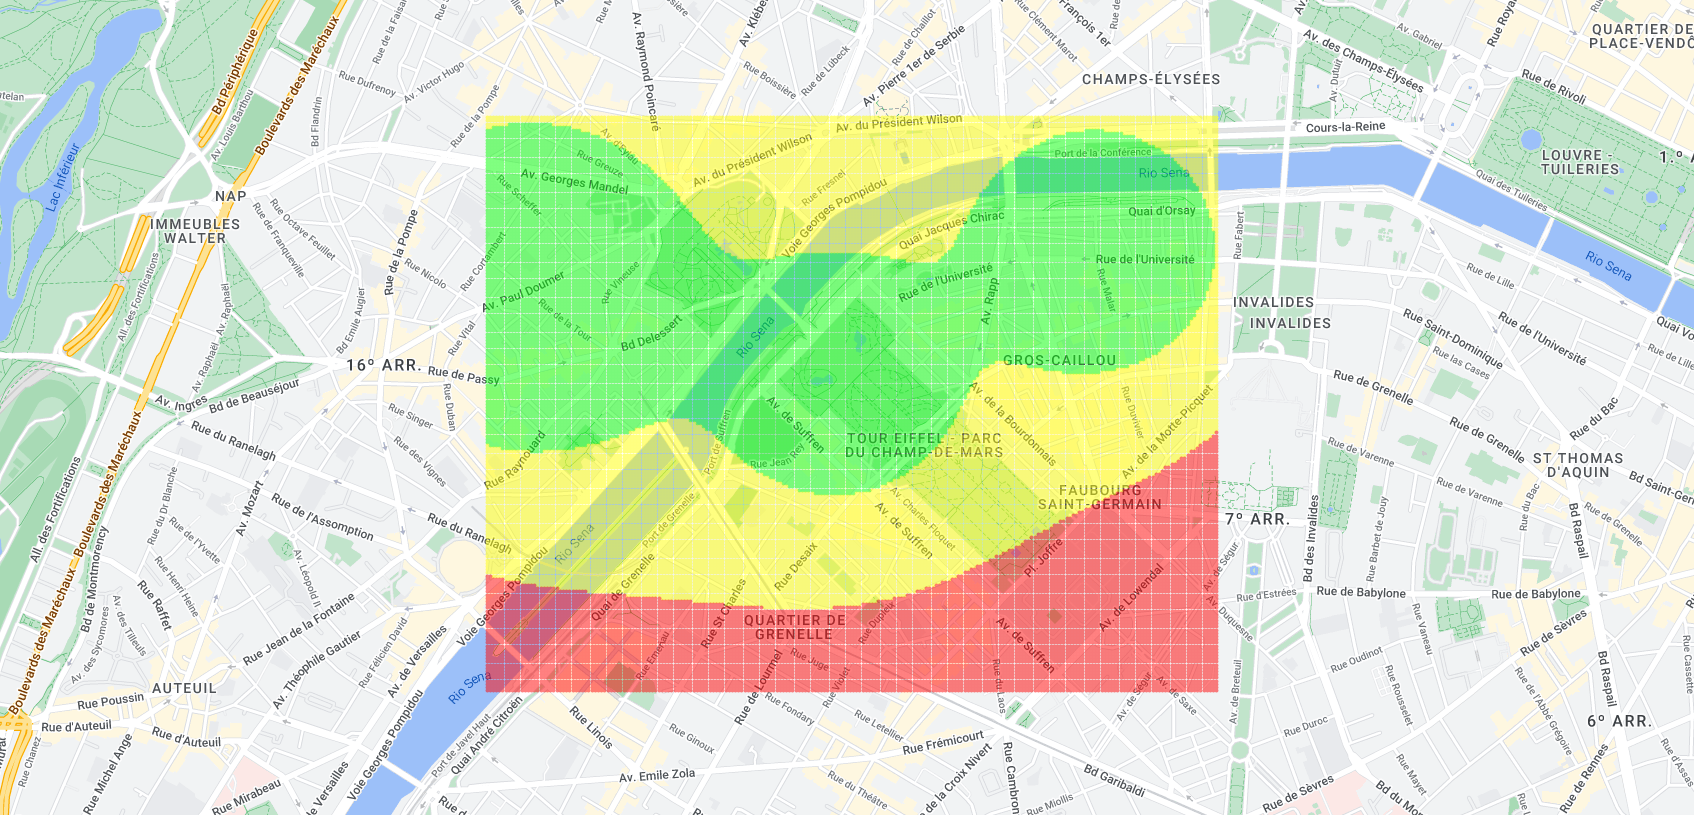
\includegraphics[width=0.9\linewidth]{Chapters/2-EDUs/images/eiffel_M3.png}
  \caption{An AoI within the city of Paris, with three different mitigation levels.}\label{Fig:zones_paris_0}
\end{figure}

When plotting the computed mitigation zones, it is defined that $ML(z_i)=1$ is green, $ML(z_i)=2$ is yellow, and $ML(z_i)=3$ is red. The maps are plotted using the Google Earth Engine (GEE).

As expected, mitigation zones will have a higher risk (red) when they are far from response-related urban infrastructure, considering only information extracted from the defined AoI. This fact leads us to consider bigger AoI, usually comprising at least the area of a city.

Figure \ref{Fig:zones_paris_3} presents an AoI comprising the central urban area of Paris, for $|M|=3$ and the same types of PoIs. A total of 801,241 mitigation zones was processed for $l = 10m$.

%%%%%% Zonas pra Paris, M = 3, AoI inteiro
\begin{figure}[ht!]
  \centering
  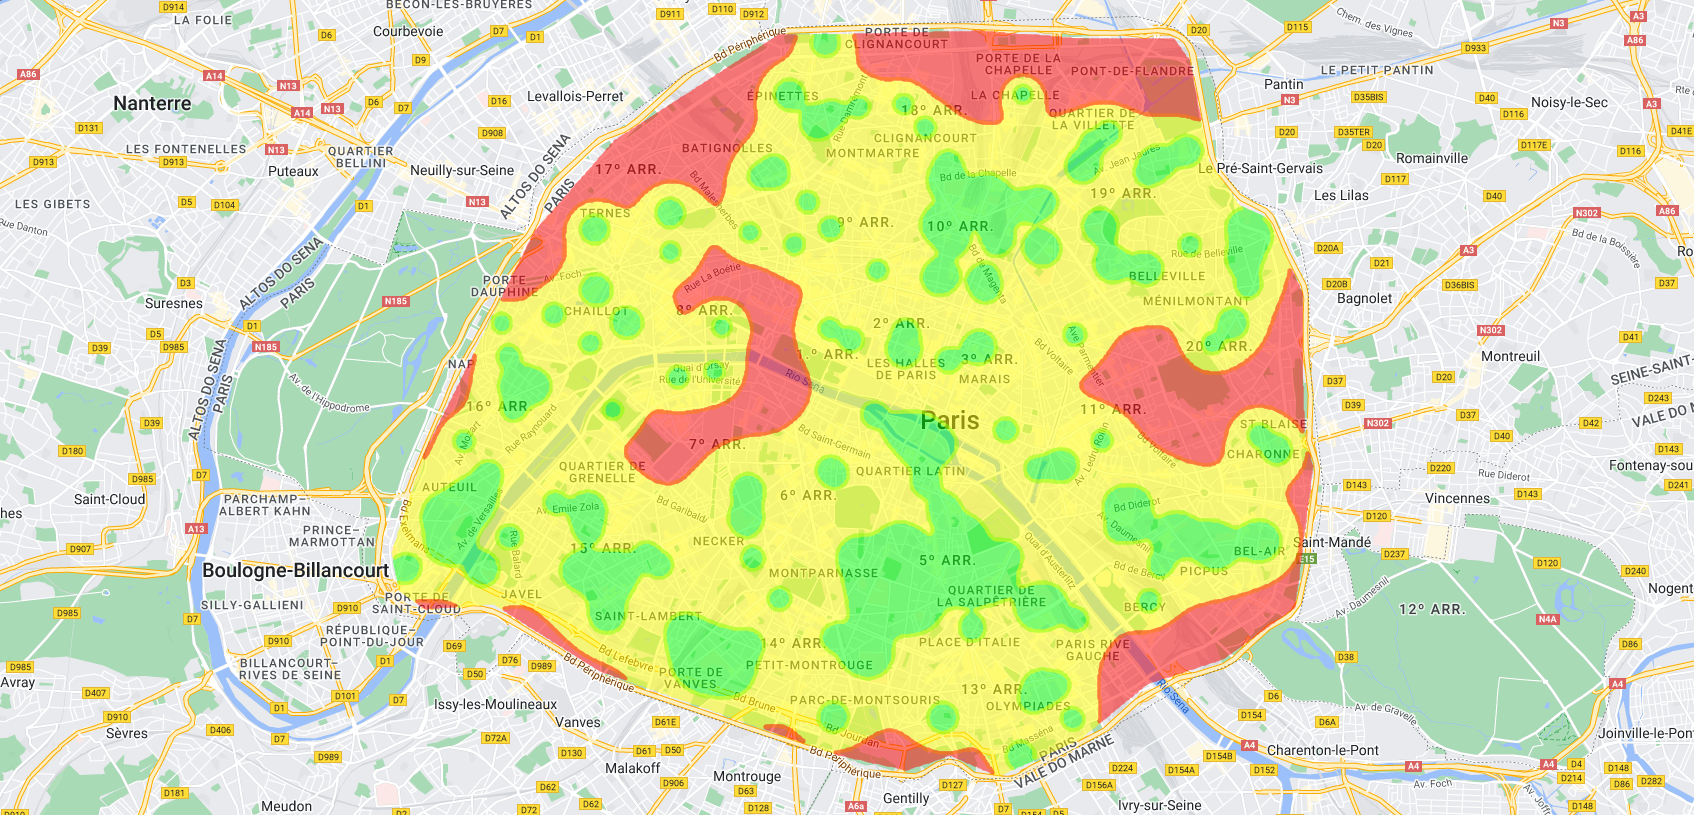
\includegraphics[width=0.9\linewidth]{Chapters/2-EDUs/images/paris_M3.png}
  \caption{A bigger AoI comprising part of Paris, with three different mitigation levels.}\label{Fig:zones_paris_3}
\end{figure}

It is important to remark that the definition of the AoI in this experiment started by the establishment of a rectangle that covered a large part of Paris. Then, all mitigation zones outside the defined limit (Boulevard Périphérique, a road ring) were removed, resulting in the actual AoI for processing. This particular reconfiguration was done as a pre-processing phase in step 1 of Figure \ref{Fig:figFluxograma}. In fact, this is an option that will depend on the intended modelling of a city, according to the expected level of precision (size of the zones) and processing costs. In the performed experiments, we might decide to consider the contours of the cities in order to better highlight the positioning of EDUs, but any configuration for the AoIs are possible.

%%%%%%%% Zonas pro Porto, M = 3
Still addressing the computation of mitigation zones, the city of Porto (smaller than Paris) was considered for $|M|=3$ and with a list of PoIs comprised of hospitals, police stations, fire departments, and metro stations. All PoIs are assumed to have the same weight in this experiment, in the same way of the evaluations for Paris. Figure \ref{Fig:zones_porto_3} presents the achieved result. 

\begin{figure}[ht!]
  \centering
  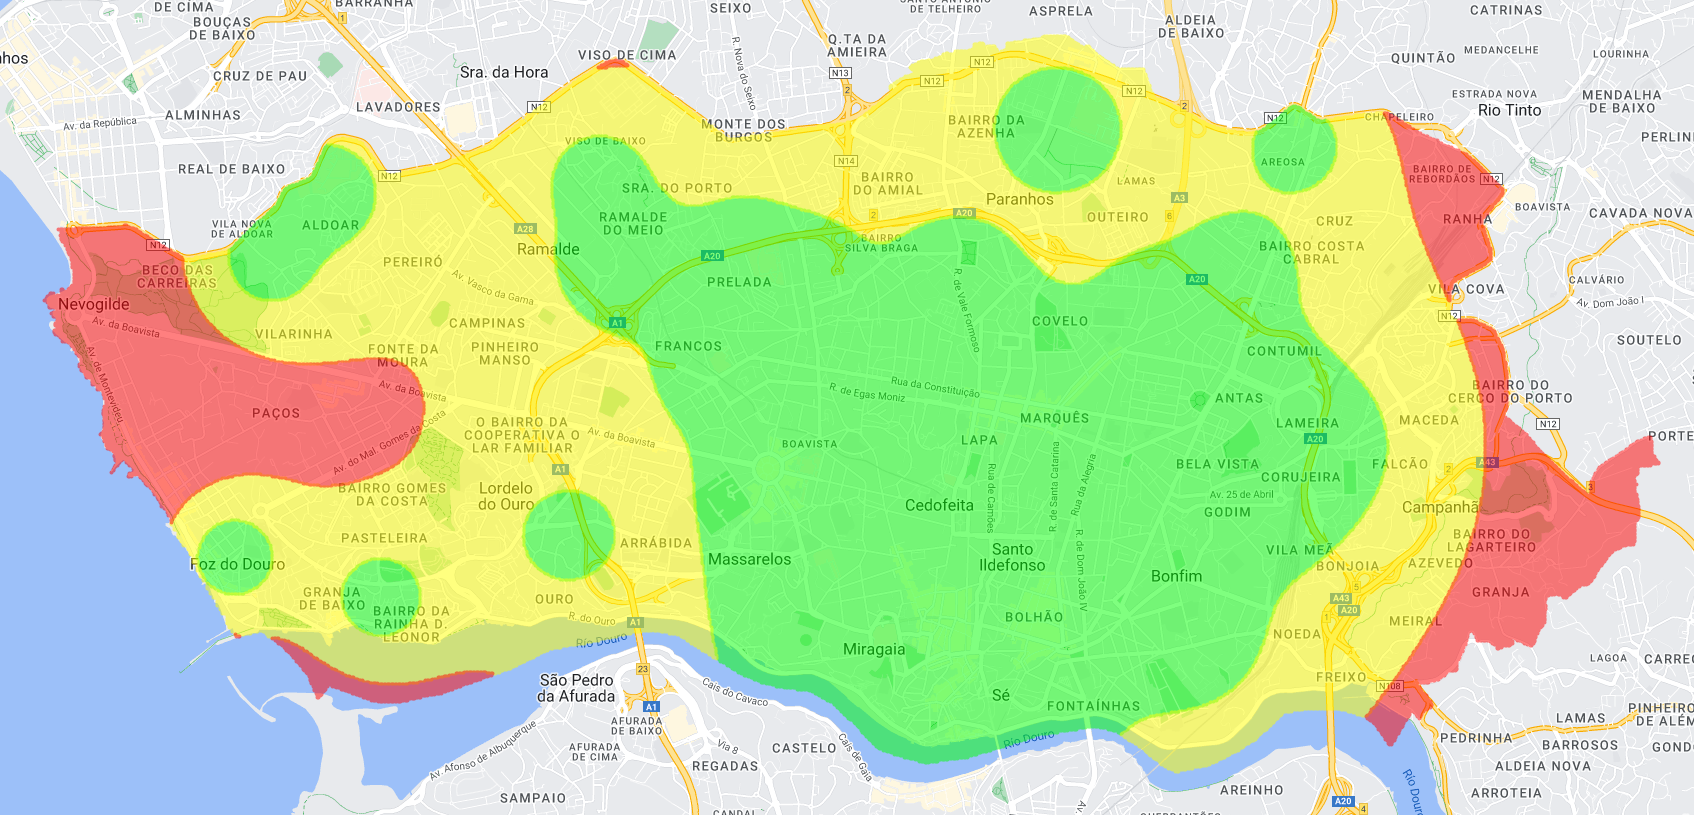
\includegraphics[width=0.9\linewidth]{Chapters/2-EDUs/images/porto_M3_no_weight.png}
  \caption{Computed zones for the city of Porto, with three different mitigation levels.}\label{Fig:zones_porto_3}
\end{figure}

%%%%%%% Zonas pro Porto, M = 5
Figure \ref{Fig:zones_porto_5} presents the same input parameters, but now defining $|M|=5$ for the same list of PoIs.

\begin{figure}[ht!]
  \centering
  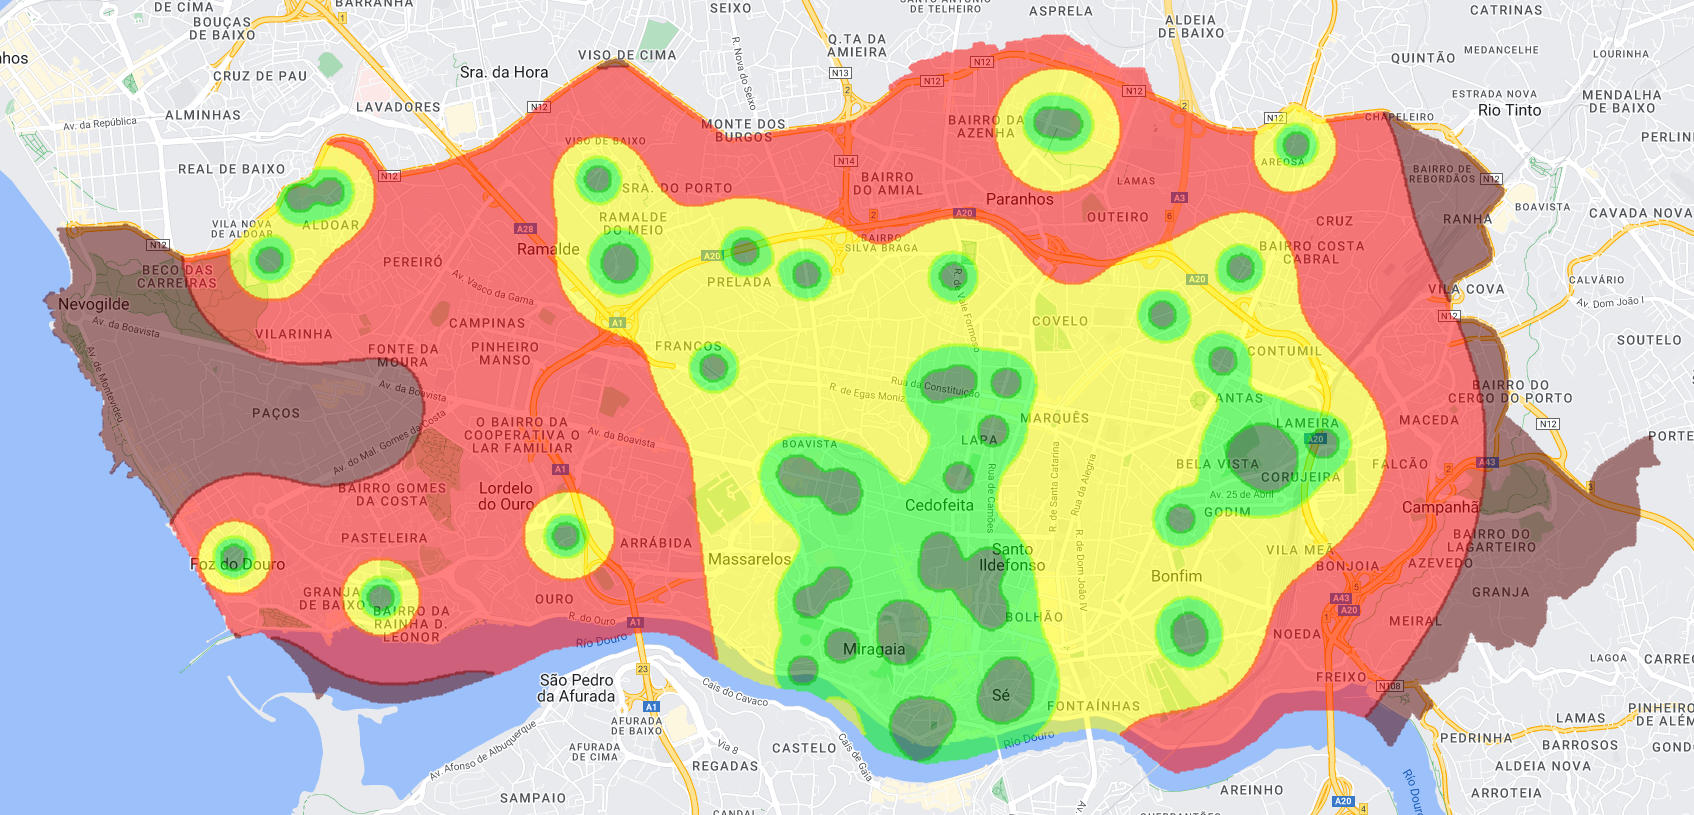
\includegraphics[width=0.9\linewidth]{Chapters/2-EDUs/images/porto_M5_no_weight.png}
  \caption{Computed zones for the city of Porto for five different mitigation levels, with dark-green representing the lowest risk while dark-red is the highest.}\label{Fig:zones_porto_5}
\end{figure}

It is interesting to notice that for higher values of $|M|$, the city is divided into more mitigation levels, but the practical outcome for sensors positioning may be not very different. Since we are using a natural logarithmic scale (Equation \ref{eq:risk_class}), the number of safer zones will be reduced, but the overall ``shape'' of adjacent mitigation zones will be almost the same, as we can see when comparing Figure \ref{Fig:zones_porto_3} and Figure \ref{Fig:zones_porto_5}. This way, after different tests for both Porto and Paris, with $|M|$ ranging from 2 to 10, we believe that $|M|=3$ may be a more usual configuration, defining three levels of criticality (bad, medium and good), which is very common in emergencies management systems \cite{surveyEmergencies}.

As an important remark, the adoption of a natural logarithmic scale in Equation \ref{eq:risk_class} creates a radial behaviour for sensors monitoring, usually irradiating from the cities' central areas where most emergencies-response facilities are located. We argue that this configuration for the mitigation zones may be more meaningful for EDUs positioning, but future works could adopt a scalar scale instead. Whatever the case, this could only change the computing of the mitigation levels, with no direct impact on the definitions of the proposed mathematical model and algorithms, leaving this choice for future evaluations.

Other set of experiments was concerned with the relevance weight of the points of interest. Figure \ref{Fig:zones_porto_3_weight} presents one of the results when $|M|=3$, assuming that $f(p)=10$ for hospitals, $f(p)=5$ for fire departments, $f(p)=2$ for police stations, and $f(p)=1$ for metro stations, considering that all PoIs of the same ``type'' have the same relevance weight. Since we have the definition of a MZ as $l = 10m$, we had 413,012 mitigation zones computed for the city of Porto.

%%%%%% Zonas para Porto, M = 3, PoI com diferentes weights
\begin{figure}[ht!]
  \centering
  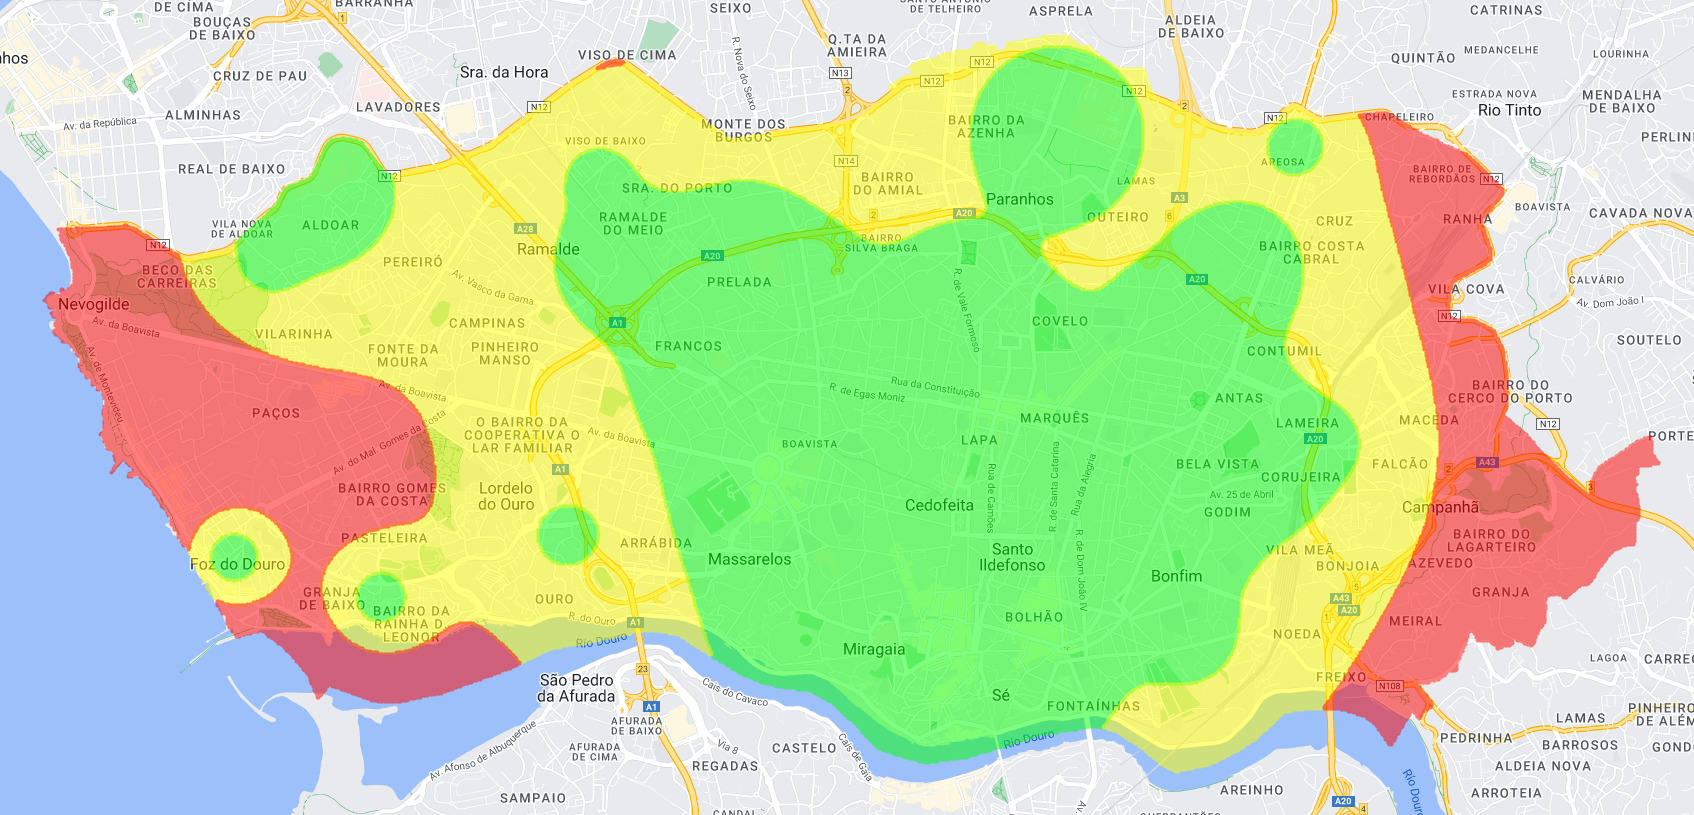
\includegraphics[width=0.9\linewidth]{Chapters/2-EDUs/images/porto_M3.png}
  \caption{Computed zones for the city of Porto, with $|M|=3$ and different relevance for the list of PoIs.}\label{Fig:zones_porto_3_weight}
\end{figure}

The weight of a PoI has the function to better set the relevance for mitigation responses in a city and thus this allows that the particularities of the selected urban area will be properly considered in the modelled scenario. Obviously, such settings will allow not only a differentiation of the types of response-related facilities, but also the configuration of a particular PoI relevance over others of the same type (e.g. when a particular hospital is bigger or better equipped than others). Doing so, the proposed approach assures a significant level of flexibility when modelling cities and emergencies management systems.

After all performed experiments, we achieved two different conclusions: first, considering practical adoption of mitigation zones in a city, $|M|=3$ seems to be the ideal configuration parameter to guide the positioning of EDUs; second, the relevance weights of the PoIs are more effective when there are some response centres that are notably much more relevant than others, once their actual positions seemed to play a more relevant role when computing mitigation zones than their relevance weights.  

%%%%%%%%%%%
\subsection{EDUs positioning}

After computing the mitigation zones for different parameters, the proposed EDUs positioning algorithms could be evaluated. For that, in order to create a uniform reference for comparison purposes, the mitigation zones created for the city of Porto when $|M|=3$ were considered, as depicted in Figure \ref{Fig:zones_porto_3_weight}. We assume the same weight configurations in that Figure, which is $f(p_h)=10$, $f(p_f)=5$, $f(p_p)=2$, and $f(p_m)=1$, for all $p_h \in P$ as hospitals, $p_f \in P$ as fire departments, $p_p \in P$ as police stations, and $p_m \in P$ as metro stations. Additionally, it is defined that $U=300$ for all experiments.

Figure~\ref{Fig:edus_random} presents the graphical results for the proposed Random algorithm.

\begin{figure}[htbp!]
  \centering
  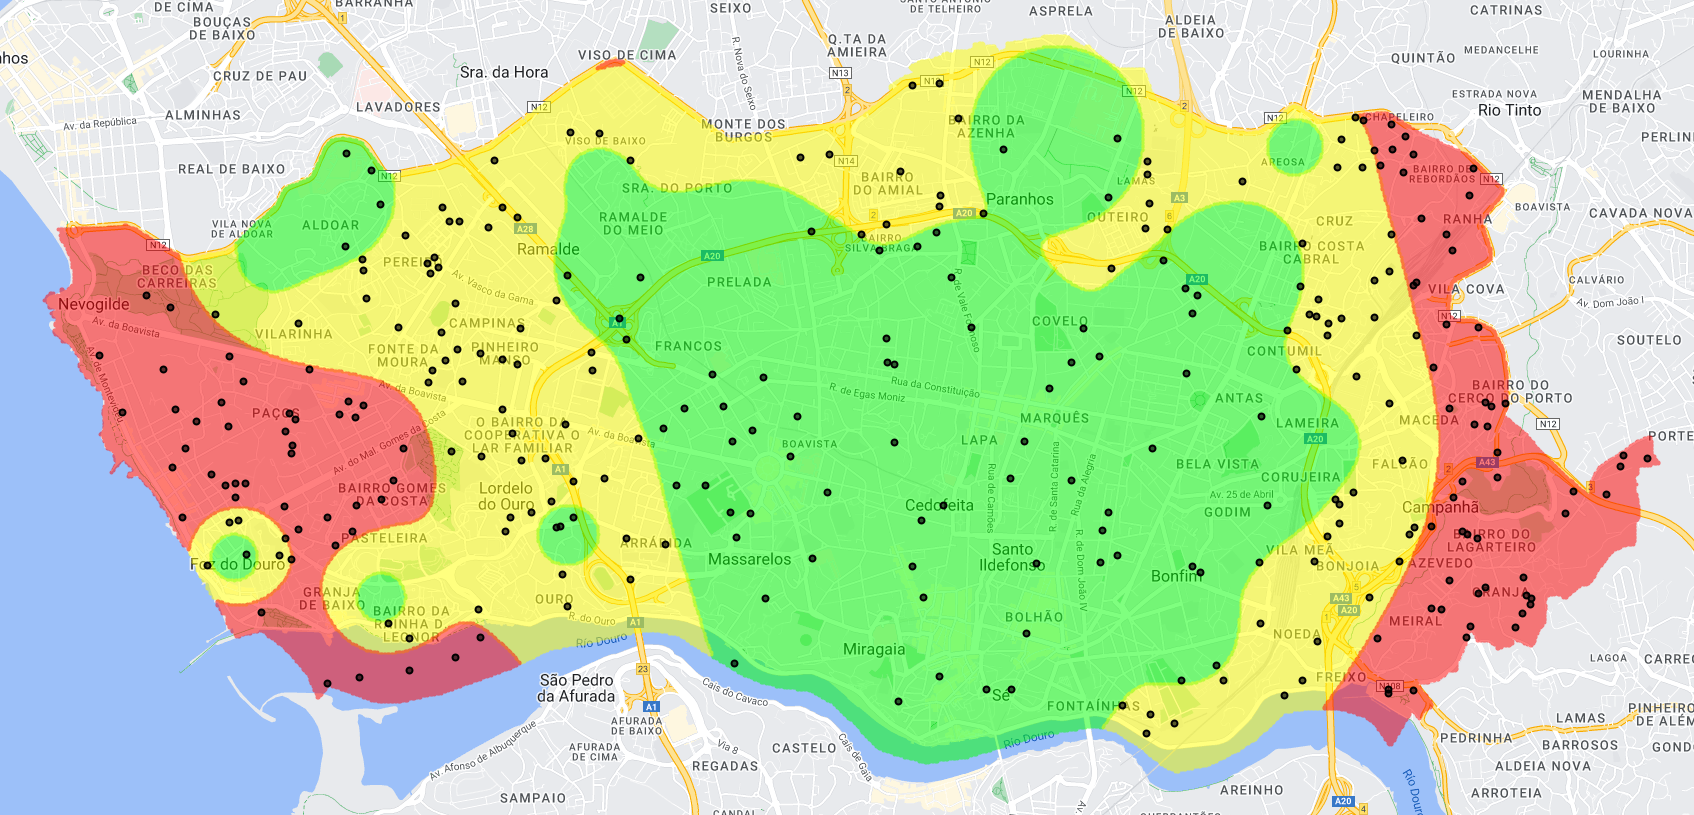
\includegraphics[width=0.9\linewidth]{Chapters/2-EDUs/images/porto_M3_random.png}
  \caption{Random positioning algorithm.}\label{Fig:edus_random}
\end{figure}

As expected, the randomly positioned EDUs do not have any specific criteria for positioning, leading to some undercovered areas and overlapping. In that Figure, the black spots are the suggested computed positions for deployment of the available EDUs.

In order to address most problems of the Random positioning approach, the Balanced algorithm was assessed in the same scenario, as presented in Figure~\ref{Fig:edus_balanced}.

\begin{figure}[htbp!]
  \centering
  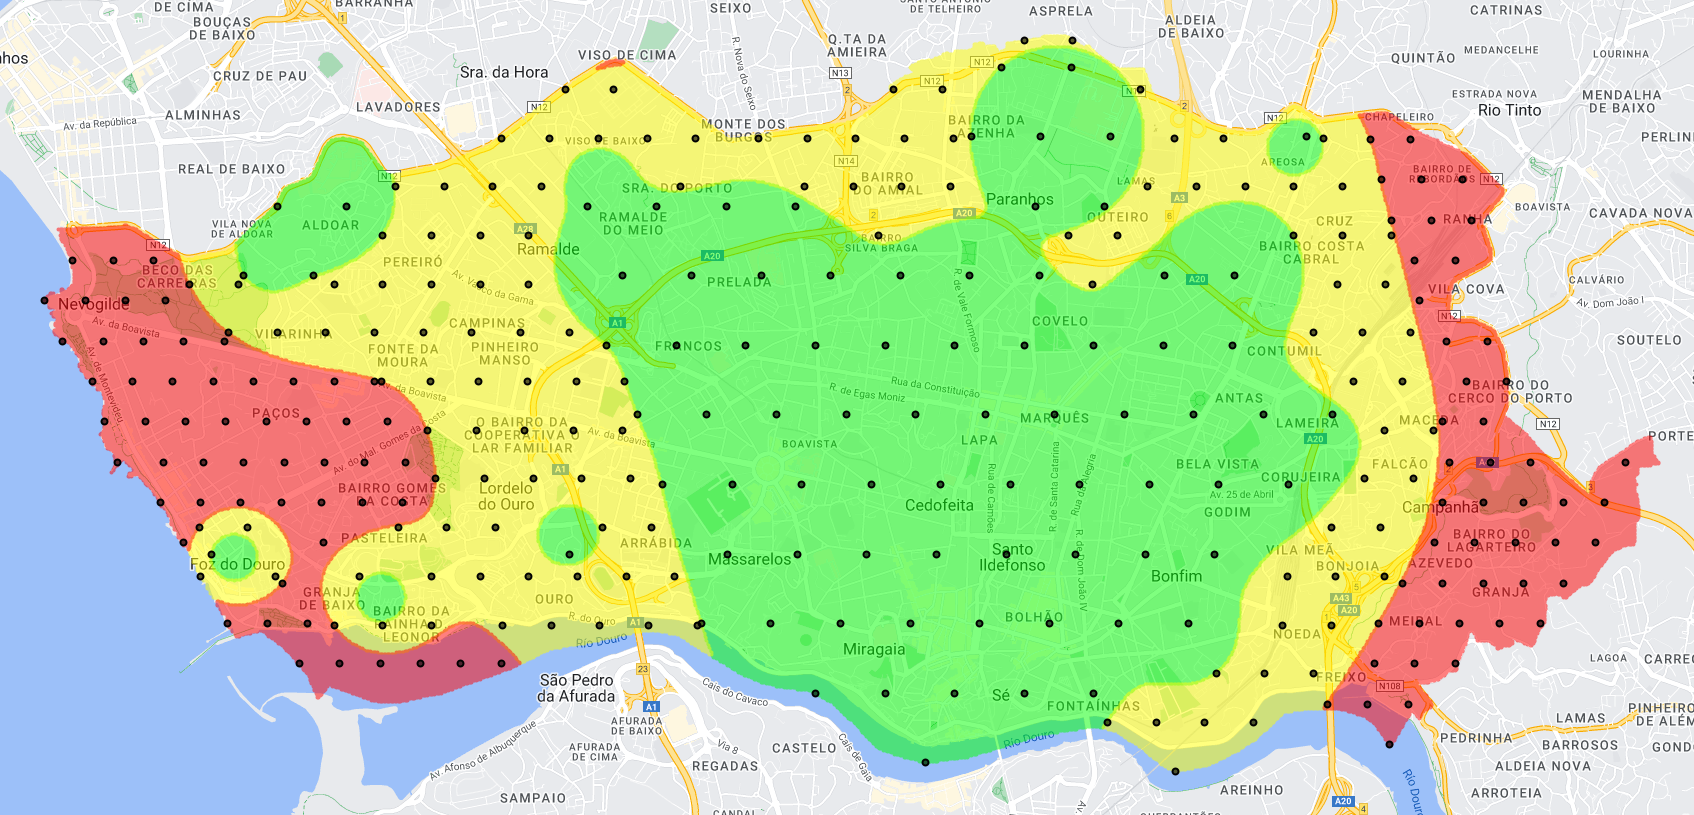
\includegraphics[width=0.9\linewidth]{Chapters/2-EDUs/images/porto_M3_balanced.png}
  \caption{Balanced positioning algorithm.}\label{Fig:edus_balanced}
\end{figure}

The Balanced algorithm performed better, but some EDUs were positioned very close to other units around the borders of the zones. Figure~\ref{Fig:edus_enhanced} presents the Balanced+ algorithm, which overcomes these drawbacks.

\begin{figure}[htbp!]
  \centering
  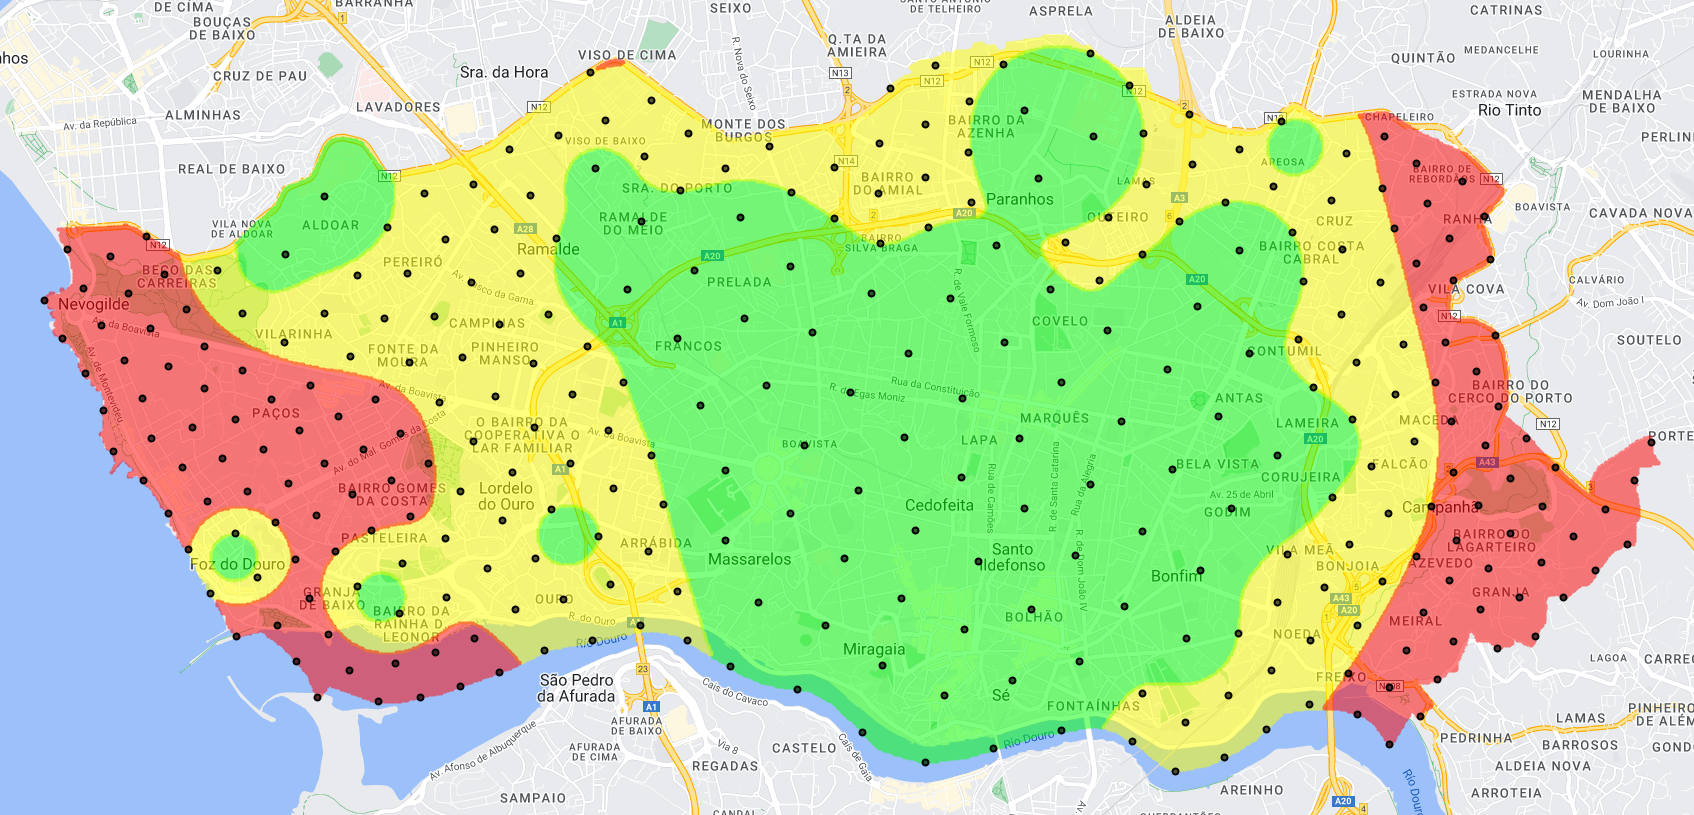
\includegraphics[width=0.9\linewidth]{Chapters/2-EDUs/images/porto_M3_balanced_plus.png}
  \caption{Balanced+ positioning algorithm.}\label{Fig:edus_enhanced}
\end{figure}

Finally, Figure~\ref{Fig:edus_restricted} presents the results for the Restricted algorithm, which we expect to have the most realistic outcome. Now, the EDUs are only positioned on allowed spots, for example avoiding that EDUs are positioned over the water as it may happen in the other algorithms.  

\begin{figure}[htbp!]
  \centering
  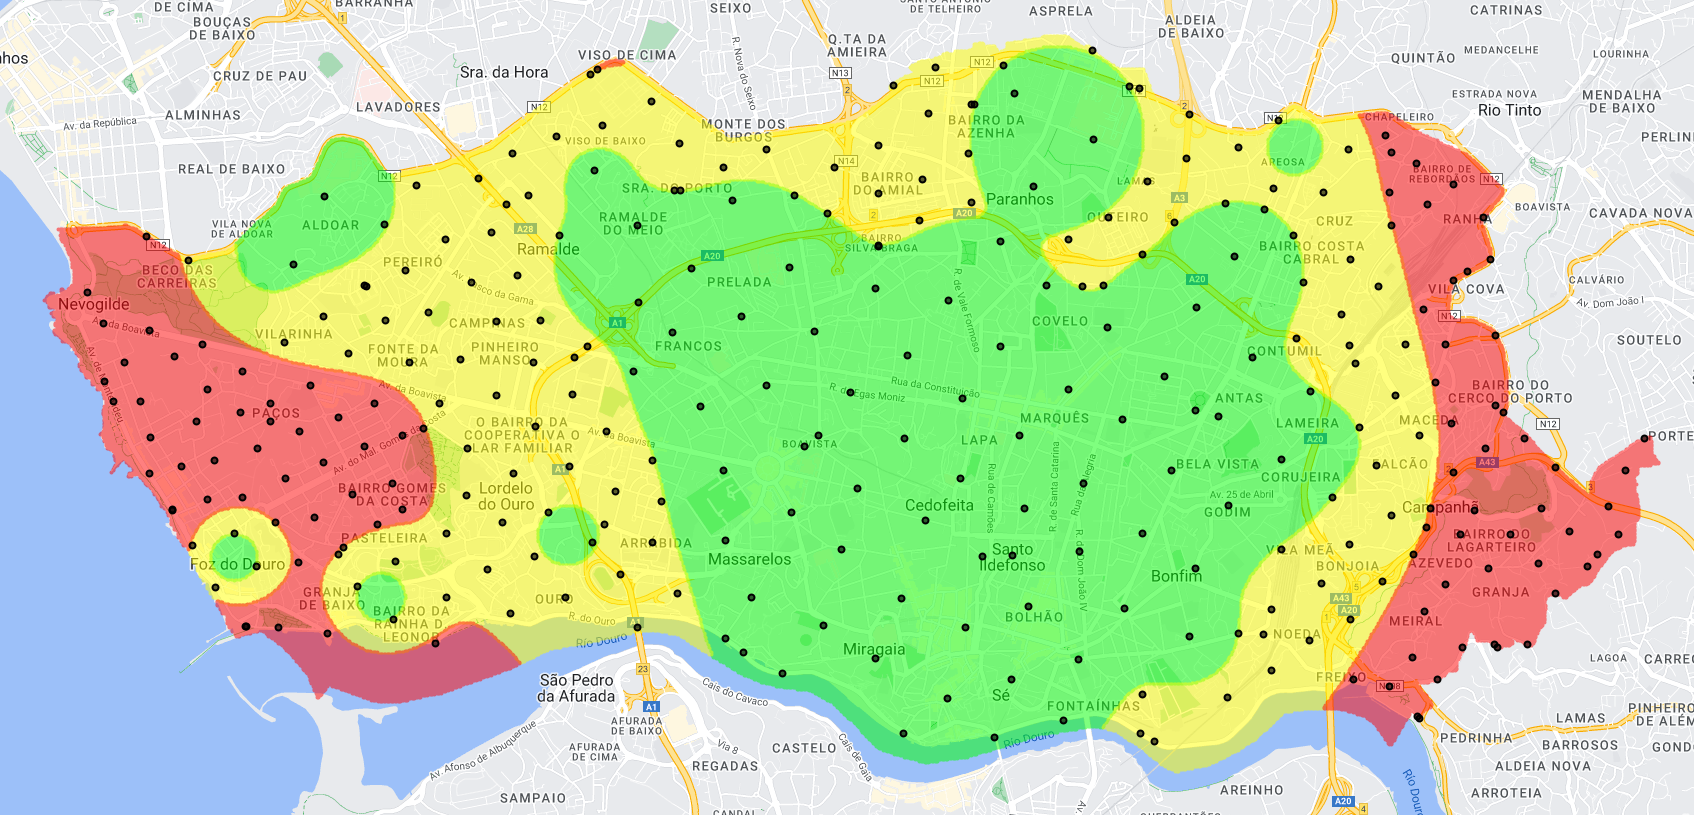
\includegraphics[width=0.9\linewidth]{Chapters/2-EDUs/images/porto_M3_restricted.png}
  \caption{Restricted positioning algorithm.}\label{Fig:edus_restricted}
\end{figure}

When comparing the different results for the Balanced+ and the Restricted algorithms, it is possible to note that the positions of the EDUs are almost the same, varying in just a few meters according to the existence of roads (more realistic spots for deployment of the units). However, such small difference achieves a more realistic result, which should be considered for actual deployment in most cases.

%%%%%%%%%
\subsection{Practical issues and performance evaluations}

When analysing the achieved experimental results with real data from two different large cities, it is possible to see that more critical areas concerning mitigation response will receive more sensors than less critical areas, which may reduce the time between effective detection and response to emergencies. Actually, this is an average reasoning about how emergencies management systems can be deployed, but it already opens new possibilities when planning such systems. Since the proposed mathematical model fits to the particularities of any city, and real OpenStreetMap data is processed as input, the proposed approach as a whole could be applied to any city in the world, which is in fact one of the major goals of this work. The performed evaluations for two different cities concerning both size and urban infrastructure are important demonstrations of the applicability of the proposed approach, which can consider not only any city as input, but also different configuration parameters.

When applying the proposed approach, the size of the AoI, the width/height of mitigation zones and the number of possible mitigation levels are not only important configuration parameters that deals with accuracy, but they will also be related to the computational costs to process the algorithms. However, it is expected that the computation of mitigation levels will be performed only once, typically just after changes in the number and configurations of the list of PoIs. In fact, after computation of the mitigation zones, the chosen positioning algorithm may be executed as a response to a new number of available EDUs, achieving new configurations and helping when searching for the ideal number of EDUs for deployment in a city. 

In order to demonstrate the computational costs of the algorithms, the execution time for the experiments on an AMD Ryzen 5 4600h processor with 16 GB RAM computer was accounted. The execution time of the algorithms for both Porto ($|M|=3$ and $U=300$) and Paris ($|M|=3$ and $U=600$) are presented in Table \ref{Table:costs}.

\begin{table}
  \centering
  \caption{Execution time in seconds for the positioning algorithms.}\label{Table:costs}
  % \resizebox{\textwidth}{!}{
  \begin{tabular}{c|c|c}
    \textbf{Algorithm} & \textbf{Porto} & \textbf{Paris} \\
    \hline
    Random  &  0.124 &  0.215 \\ 
    \hline
    Balanced  & 5.692  &  10.974 \\ 
    \hline
    Balanced+  & 107.578 &  316.359  \\ 
    \hline
    Restricted  & 108.716  & 325.006 \\ 
  \end{tabular}
  % }
\end{table}

The execution time of the positioning algorithms will increase for more complex algorithms, but they will usually deliver better results. In fact, the execution of the positioning algorithms is not the most time-demanding part of the proposed approach, with most time being spent to compute the mitigation zones. For example, when having $|M|=3$, Porto (Figure \ref{Fig:zones_porto_3_weight}) took 998.46 seconds while Paris (Figure \ref{Fig:zones_paris_3}) needed 1341.99 seconds to compute all mitigation zones. At this point, as expected, we can conclude that the final computational cost will depend on multiple variables, although the processing time is not a critical situation in this problem scope.

Finally, the employed geospatial data source could be considered as an important parameter when adopting the proposed approach, affecting the overall processing time of the algorithms. Although the proposed approach is not dependent on the OpenStreetMap database, it is assumed as the reference for processing of mitigation zones, mostly due to the fact that it is an open geospatial database that is collaboratively managed and updated. As long as it is regarded as a reliable source of data to compute mitigation zones, the time needed to pre-process a city and select all PoIs was not significant when using OSM, since such list (and related metadata) was processed in few seconds. However, when other sources of data are selected, the data acquisition time and general data reliability may be important issues that have to be properly considered.

%%%%%%%%%%%%%%%%%%%%%%%%%%%%%5
\section{Discussions and perspectives}\label{S:6}

As discussed throughout this article, the positioning of the EDUs in a city is a very important issue for emergencies detection units, which reinforces the need for flexible positioning algorithms. Overall, the detection of emergencies in smart cities is the first step when handling critical situations in urban areas, and thus the proposed approach comes as a valuable pre-deployment step in such scenario. In this article, we argue that distributed sensors will be one of the main data sources when detecting emergencies, which put their proper assembling, programming, positioning, and deployment, as major issues to be improved. At this point, while the construction of emergencies detection units have been addressed lately \cite{hardware1,hardware2}, their positioning in a city still has many challenges when emergencies detection is being performed.

The four proposed algorithms presented valuable results to guide the deployment of EDUs in a city, mainly when taking the more realistic Balanced+ and Restricted algorithms. As discussed before, this is accomplished by exploiting geospatial data of emergency-response urban infrastructure, which allows the computation of real positions for the units. However, the actual deployment of the units and the issues associated to it such as physical attachment, energy supply, networking coverage, transmission throughput, among others, are out of the scope of this work since they are more related to wireless sensor networks and Internet of Things (IoT) systems than smart cities planning. Additionally, actual deployment of the EDUs would not be very significant to evaluate the proposed algorithms themselves, but it could be valuable when pursing other research goals than the ones already addressed in this work. Finally, due to the necessary cost to deploy hundreds or thousands of EDUs in a city just to evaluate the proposed algorithms, additional evaluations with physical units were not performed.

Still considering additional research issues for actual deployment, it is reasonable to expect that the EDUs will be usually deployed on the outdoors, potentially in public areas. For such deployment, EDUs could be attached to trees, electric poles, bus stops, traffic lights, among other spots. Moreover, public buildings such as schools, post offices and even the city hall could be adopted as deployment spots once they are very close to the area suggested by the proposed algorithms, facilitating actual deployment. 

Other important remark is that some networking issues such as connectivity, throughput, availability, and even security, were not considered by the proposed positioning algorithms, which might lead to disconnected EDUs in cities with poor networking infrastructures. Actually, we consider that these networking ``parameters'' should be processed in a post-positioning phase of the proposed approach, potentially supporting a fine-grained positioning of the EDUs. This way, networking would behave like a response layer, but it would not be directly used to define positioning zones. The idea would be to perform small reallocations of the EDUs within the same mitigation zones when some defined networking quality parameter is improved. In fact, we believe that networking could be incorporated to the proposed solutions through a mathematical model when the actual networking infrastructure of a city is properly known. This remark will be considered in future works.

Finally, after the performed experiments have given important clues about the practical effectiveness of the proposed approach, we could wonder about the way cities may be perceived when mitigating emergencies. Actually, the definition of mitigation zones might be perceived as a Response Layer in a more generic term, which would be only one step of a more comprehensive solution when guiding the positioning of EDUs. Doing so, for example, the average traffic accidents in an urban area could also be defined as a response layer, which would be applied after or before the processing of the mitigation response layer. And the same could be done when accounting the presence of dangerous facilities, such as a factory of dangerous chemical products, or even a nuclear station. In this same direction, the relief of a city could also be processed as a layer that could complement the 2D perspective of zones adopted in this work, for example allowing the processing of higher (or lower) areas as more/less critical for emergencies. Whatever the case, all of these conceptual layers can be processed sequentially in a balanced way, resulting in an integrated perception of risks that will ultimately result in a combined risk index for each subarea in a city. Nevertheless, although we believe that such multi-layers perception is promising, we expect that future solutions can be applied mathematically in a generic way, exploiting open geospatial data from open databases.


%%%%%%%%%%%%%%%%%%%%%%%%%%%%%5
\section{Conclusions}

This article proposed a comprehensive mathematical model and four different positioning algorithms to guide the deployment of Emergencies Detection Units in a city. For that, the concept of mitigation zone was proposed and the procedures to exploit it to position EDUs in a more efficient way were discussed. With the performed experiments, practical issues were analysed, as well as the computational costs of the solutions were accounted. At the end, the expected results of this work were achieved. 

In general, resilience to detected emergencies has been a recurrent issue when creating smart cities. At this sense, although only part of the overall emergencies management cycle was addressed in this article, EDUs positioning has not been properly considered as an actual problem for macro-system solutions that consider an entire city as a deployment area. Therefore, the proposed approach comes as an important improvement to this research area, potentially fostering new investigation efforts in the positioning and deployment of multi-sensor units in smart cities.

As discussed in the previous section, future works will be concerned with the evaluation of the proposed model in order to consider other geospatial urban data, complementing the existence of mitigation response centres. Moreover, other positioning algorithms will be proposed and evaluated, trying to better optimise the positioning of the EDUs. Finally, genetic algorithms will be considered to compute the positions of the EDUs when input parameters other than mitigation zones are considered, opening a new research trend in this area.

% \section{Acknowledgement}

% This work is financially supported by national funds through the FCT/MCTES (PIDDAC), under the project EXPL/EEI-COM/1089/2021. It is also supported by INEGI-LAETA (FCT project UIDB/50022/2020). Finally, this work was financed in part by the Coordenação de Aperfeiçoamento de Pessoal de Nível Superior - Brasil (CAPES) - Finance Code 001.

\printbibliography[heading=subbibliography]

\end{refsection}

    % --------------------------------------------------
% Capitulo 3: CityZones
% --------------------------------------------------
\chapter{CityZones: A geospatial multi-tier software tool to compute urban risk zones}\label{cap:cityzones}

\begin{refsection}

\textbf{ABSTRACT}

CityZones is an online tool to support when computing risk zones in a city, which is performed by mathematically evaluating the emergency response capability of an urban area using real data. The tool allows users to define polygonal Areas of Interest (AoI) on a map, which are categorised into low, medium, and high-risk levels. As urban emergencies in general will typically demand the assistance of hospitals (to attend victims), firefighters (for rescue operations and damages reduction), policemen (to control and manage critical situations), and even metro stations (for evacuation), the risk zones within an AoI will be computed according to the distances to such existing infrastructure, which is extracted from the OpenStreetMap database. The coordinates of an AoI are defined at the client-side and submitted to a server as a regular or irregular polygon, which is then stored in a GeoJSON file along with the computed classifications for further processing according to a multi-tier pipeline. Adopting a configurable square-based mathematical model to compute distances and relative risk levels, the risk zones are computed on-demand and exported to CSV files to be used by any application, with an additional representation for web-based visualisation. Moreover, as a practical exploitation of the computed maps, the CityZones tool also suggests ideal positions for sensors-based Emergency Detection Units (EDUs) within an AoI according to the chosen positioning algorithm, assuming that the computed risk zones indicate how severe an undetected emergency would be. While the CityZones tool is not intended to provide a mitigation approach at all, since it does not have knowledge about current emergency situations, it stands as a valuable pre-mitigation tool to be used in the planning phase of emergency management in smart cities, bringing an important contribution for practical applications in this area.

\textbf{Keywords:} Geospatial data, Urban emergency, Smart cities, OpenStreetMap.

\section{Motivation and significance}

The problem of emergency management in cities can be strongly supported by risk maps that identify zones where eventual critical situations are potentially more severe~\cite{mapping1}. In practical means, risk maps may indicate the level of urgency for emergency detection in an area, as well as which mitigation services are more required to respond an emergency~\cite{surveyemergencies1}. With such information, stakeholders could have a more practical perspective of the current distribution of emergency-response facilities in a urban area, as well as planning of emergency management systems could be significantly facilitated. In this scenario, the challenge has been to identify programmable ways to compute risk zones for any defined area in the world, in a cost-effective way, better preparing a city to the occurrence of emergencies. In fact, although the proper mitigation of an ongoing emergency is not in the scope of the tool, the provided information can support other tools with knowledge about emergency mitigation infrastructure..

Given the unpredictable nature of emergency situations, it is important to assess the expected level of resilience of urban areas in the aftermath of an emergency, with a focus on the presence of emergency mitigation facilities. In our previous work~\cite{riskzones}, we proposed a mathematical model for computing urban risk zones by partitioning an Area of Interest (AoI) into small, continuous squares arranged in a grid-like configuration, which are referred to as Mitigation Zones (MZ). Each MZ is then classified into one of three risk levels (low, medium, or high), based on the relative impact of potential emergencies such as fire, flooding, and earthquakes, and considering the distances from existing mitigation facilities such as fire departments, hospitals, and police stations, each defined by a GPS coordinate as a Point of Interest (PoI). Although our previous work established a flexible mathematical model, further improvements are required to create a more practical tool for addressing real-world problems.

%%%
CityZones is an open-source multi-tier platform that allows users to select any regular or irregular polygonal AoI through a web interface, as well as a set of configuration parameters, allowing the computation of risk zone maps based on the existence of different types of mitigation infrastructure. Such selection in Tier 1 is supported by a JavaScript library that directly access data from the OpenStreetMap for visualisation. Users select any configuration parameters and submit a ``risk zones computation request'' (task) to a cloud-based server through a web interface, which comprises the Tier 2. Then, the received clients' tasks are inserted into a processing FIFO pipeline, with the oldest task being served by the defined algorithms in a sequential way. At a dedicated server at the University of Porto (Tier 3), a file sizing 67~GB containing the metadata of all elements in the OpenStreetMap database was already processed to include only the Points of Interests (hospitals, fire departments, police stations and now also metro stations), for all cities in the world, resulting in a final file sizing 22~GB. This processed file and the clients' requests are the input parameters for the algorithms that will compute the risk zones. The Tier 3 server periodically requests a new task to the cloud-based web server (Tier 2), receiving as response the set of configurations of the first request on the FIFO queue. After running the defined computation algorithms, the Tier 3 server sends back to the cloud server the results in the CSV format containing the classification of each zone, as well as other eventual requested results.

In addition to computing risk zone maps, the CityZones tool can also suggest potential positions for sensor-based Emergency Detection Units (EDUs). To detect emergencies, many cities rely on affordable multi-sensor detection units that monitor various variables and identify abnormal conditions~\cite{sensorsedus,sensorsedus2}. However, deploying a certain number of detection units is not enough; the challenge lies in determining the proportional number of sensors in each region and their optimal position based on the unique characteristics of a city. By classifying different areas according to their risk levels (risk maps), the CityZones tool can compute the proportional risks of each zone and suggest EDU positions accordingly.

This article describes the conceptual structure and the development challenges of the CityZones tool. Practical examples and performance evaluations are also presented, better supporting its adoption in smart city scenarios.

%%
\section{Related works}

In general, supportive tools to facilitate processing of geospatial data are not a novelty, with some works already presenting valuable results in this area~\cite{geospatial1,geospatial2,simulationflood}. When coming to the processing of city-related metadata, the literature has presented some valuable results of how such tools can be helpful in multiple scenarios~\cite{geospatial3,geospatial4}. Actually, the adoption of crowd-sourced geospatial databases has significantly increased in recent years~\cite{geospatial5,geospatial6}, with OpenStreetMap having a great relevance in this scenario as a reliable source of completely access-free geospatial data~\cite{osm}.

Some other works have made proposals to analyse environmental data and classify areas regarding emergencies. In~\cite{classificacao1_calor}, for example, the authors have used the heat-related mortality history in some USA cities to create a correlation between demographic and environmental variables to the risk of dying during hot seasons. The work in~\cite{classificacao2_clima} proposed a resilience index that makes use of several demographic parameters to classify an area into low, medium or high resilience, creating a resilience map of a city. Another example is the work in~\cite{classificacao3_redi}, that also proposed a resilience index based on demographic and environmental data to classify the resilience of a city.

All these works perform some risk or resilience classification of an area so that it could be leveraged by stakeholders when better planning emergency response actions in a city. However, there are some restrictions: for example, the work in~\cite{classificacao1_calor} is specific for heat-related mortality, while the works in~\cite{classificacao2_clima} and~\cite{classificacao3_redi} are more generic, but they rely on data data from specific regions. In this sense, CityZones comes as a tool that integrates multiple services that are based on previous works, creating a configurable multi-tier processing service that provides risk zones maps for any requesting smart city application, relying on publicly available and unbiased data.

%%%%%%%%
\section{Software description}

\subsection{Software architecture}

The defined architecture for the CityZones tool was designed to allow easy access by the users through a powerful but lightweight interface, which is supported by different services with well-defined processing loads. The idea is to achieve a consistent architecture that can be implemented in multiple ways, once the main requirements and conceptual organisation are respected.

The three conceptual tiers of the tool are: Client (Tier 1), Server (Tier 2), and Maps-Service (Tier 3). Each tier will implement one or more software \textit{modules} that will have a well-defined function. Figure~\ref{fig:flow} presents such expected flow in 9 processing steps ($S1$ to $S9$).

\begin{figure}[htb]
  \centering
  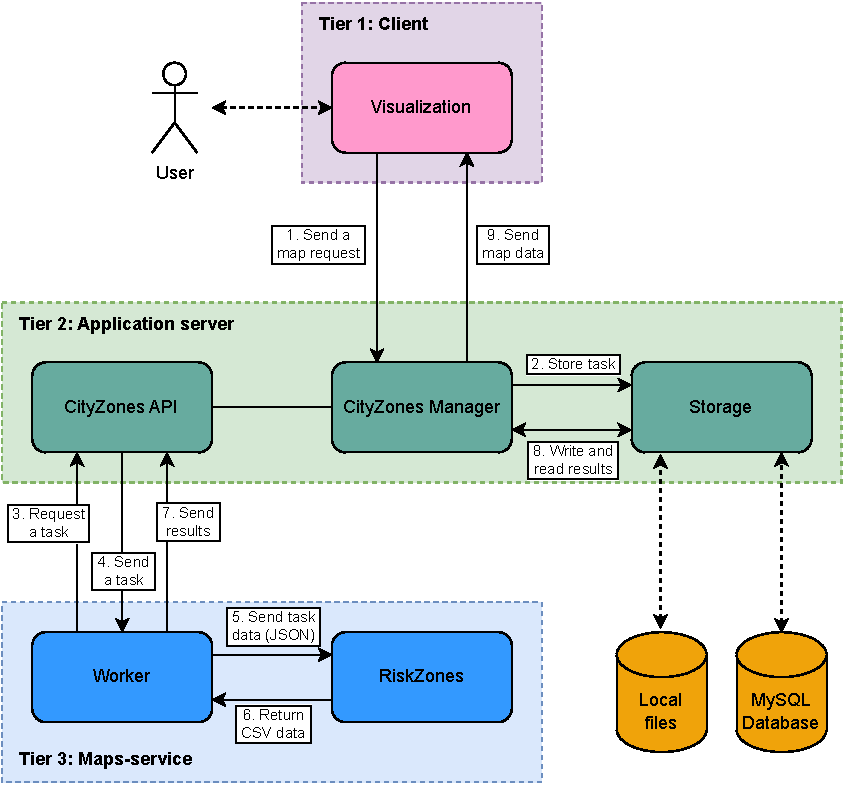
\includegraphics[width=\linewidth]{Chapters/3-CityZones/img/fluxograma_webapp.pdf}
  \caption{Processing flow through the defined modules.}\label{fig:flow}
\end{figure}

%%%%%%
\subsubsection{Tier 1 - Client}

The Client is implemented as a conventional web application to be accessed through a web browser, comprising a visualisation module to handle maps, to display configuration options, and to present the computed results. This module interacts with the application server through the browser, sending requests ($S1$), and receiving computed maps ($S9$) that are then displayed to the user.

The visualisation module will present an interface with a navigable map so that the user can interact with it dynamically, defining the polygon of the AoI and any related parameters (size of the MZ, relevance of each type of PoI, and number of EDUs for deployment). Additional functionalities to facilitate the interaction of the user with the CityZones tool will be also available in this module.

The user interface module was specifically designed to make our proposed algorithms accessible to a wide range of stakeholders, without requiring prior scientific knowledge. This module is recommended for use by public agents involved in city planning, emergency management, and disaster risk reduction, including emergency management coordinators, fire chiefs, police chiefs, EMS (Emergency Medical Services) directors, and directors of public agencies.

%%%
\subsubsection{Tier 2 - Application server}

This tier is implemented as a cloud-based server that is responsible for receiving the users' requests in the form of ``tasks'', managing a FIFO queue of such received tasks, providing an interface to access them, and transmitting the computed results to the client. A task is a client's request to compute a risk zone, considering all associated metadata for that, which is stored until it is requested by a Maps-service device. This architectural configuration allows the implementation of any number of Maps-services, supporting when multiple clients' requests have to be processed within a short period of time.

A task, which is a core element in the software architecture, can be represented by the tuple ($id$, $created\_at$, $requested\_at$, $requests$, $description$, $config$, $geojson$), as described in Table~\ref{tab:task}.

\begin{table}[h]
  \centering
  \begin{tabular}{p{.2\linewidth}p{.7\linewidth}}
    \hline
    \textbf{Parameter} & \textbf{Description} \\
    \hline
    $id$            & The ID of the task, used for its identification when sending and receiving tasks from a Maps-service worker \\
    $created\_at$   & The timestamp of the creation time of the task \\
    $requested\_at$ & The timestamp of the last time it was sent to a Maps-service worker \\
    $requests$      & How many times this task was sent to a Maps-service worker \\
    $description$   & The user-defined description of the task \\
    $config$        & The JSON configuration of the task (contains the boundaries of the grid, zone length, number of EDUs, positioning algorithm and weights of the PoIs) \\
    $geojson$       & The GeoJSON defining the polygon of the AoI \\
    \hline
  \end{tabular}
  \caption{The parameters of a task.}\label{tab:task}
\end{table}

The Application server will be composed of three modules. The first module (CityZones Manager) will handle the overall operation of the server, orchestrating the operation with the other modules. First, it will receive requests to compute risk zones ($S1$) and reply with the corresponding results when they are ready ($S9$). Moreover, the manager module will control the storage of tasks and computed maps, as well as the access to the CityZones API by the Worker module of any number of Maps-service workers. The Storage module will control the access to the database and local storage (steps $S2$ and $S8$), according to the type of data being considered. Finally, the CityZones API module provides the interface so any Maps-service worker receives tasks ($S4$) and sends back the results ($S7$) in an asynchronous way.

%%%%
\subsubsection{Tier 3 - Maps-service}

A Maps-service is expected to be implemented on a ``powerful'' computer to perform the computation of the risk zones, and more than one Maps-service may be implemented to support the CityZones tool.

Two modules are implemented by a Maps-service. The first module (Worker) sends a request for a task ($S3$) and receives the definition of a task to be processed ($S4$) from the application server. After $S3$, it starts processing the received task, extracting the AoI from the OpenStreetMap global data. Then, the second module (RiskZones) is executed ($5$), which computes the risk zones for the AoI and (if requested) the positions of the EDUs for the set of computed zones. Once the results are ready for a particular task ($S6$), the Maps-service sends it back to the application server ($S7$), asynchronously, which will store the resulting CSV files (computed maps) on its local storage ($S8$), as well as any associated metadata to the MySQL database.

%%%%%%%
\subsection{Software implementation}

Different technologies and programming tools were employed to implement CityZones. The Client is a web application that users can access through a web browser, requiring a minimum support to JavaScript. The map interface displayed on the web client is powered by Leaflet~\cite{leaflet}, a JavaScript library that provides a graphical interface for maps. When results are ready, the JavaScript code (retrieved from the application server and executed on the browser) will load the OpenStreetMap image data for map previewing, allowing very intuitive and visual interactions with the users.

The Application server was written in the Python~3 programming language on the Flask framework~\cite{flask}, which provides an easy-to-start environment for web applications. The server codes run on the cloud-based hosting service Dreamhost~\cite{dreamhost}, although any cloud hosting service or UNIX-like server with Python~3 and WSGI Phusion Passenger~\cite{phusion} support for application loading could be employed. Concerning the implemented database, the available MySQL service~\cite{mysql} on the same hosting service was adopted to store the tasks and other relevant metadata. The Application server is a monolithic application that provides the views for the Client.

The Maps-service modules (Worker and RiskZones) are also written in the Python~3 programming language. Concerning this Tier, the Worker module loops forever, while the RiskZones module is executed when requested. The interactions between the Worker module and the Application server through its CityZones API are performed through the REST API.

Any Linux system that supports Python~3, the Osmium command line tool~\cite{osmium} and with the complete OpenStreetMap PBF data file can run the Maps-service modules. To avoid vandalism and unauthorised access, an API key must be set in both the Application server and the Maps-service Workers, so only systems with the correct key can request tasks and transmit results.

%%%
\subsubsection{Files formats}

The configuration for the RiskZones module is given by the Application server in the JSON format (JavaScript Object Notation)~\cite{json}, while the AoI delimitation is provided by the Application server in the GeoJSON format~\cite{geojson}.

When an user requests a new task on the map view, CityZones creates a JSON configuration file and a GeoJSON of the AoI so that the RiskZones tool can use them to process the classification and EDUs positioning. This processing is performed on the Maps-service side. The CityZones tool provides access to the JSON and GeoJSON files generated through the download link that appears at the task's row on ``Tasks'' view, indicated with a down-arrow on a file icon. By clicking in the configuration download link, CityZones will send to the browser a ZIP file containing both JSON and GeoJSON files so that the user can decompress it and run RiskZones tool via command line (if desired). These files allow the user to make modifications to the configuration of the task and run it locally. It is important to notice that this approach requires an OSM or PBF file containing the AoI to be classified. Such file can be exported via OpenStreetMap web interface or downloaded from Planet OSM~\cite{planetosm}.

Another download link indicated by a CSV acronym on a file icon allows the user to download the results of the task. The downloaded ZIP file contains three files: the map CSV for the zones classification, the EDUs CSV for the EDUs positions and the roads CSV for the roads and streets detected in the AoI (this data is used for EDUs restricted positioning). These CSV files can be imported as assets into Google Earth Engine or any other GIS software.

%%%%
\subsubsection{Computing risk zones}

The first step that a Maps-service worker will take after receiving a task is to get its AoI polygon to extract its data from the OpenStreetMap reference data file. That data file is a 67~GB PBF (Protocolbuffer Binary Format) file containing data of the whole world, directly downloaded from the OpenStreetMap collaborative database. Actually, it can be reduced manually by running \emph{osmfilter}, a OpenStreetMap command line tool that filter data from a PBF or OSM file, potentially facilitating processing of geospatial data based on it. Since the initial version of the CityZones tool is currently considering only hospitals, fire stations, police stations, metro stations and roads for classifying zones and positioning EDUs, the file that is actually used by a Maps-service worker is a filtered PBF file with 22~GB of data.

For AoI extraction, a Maps-service worker uses another command line tool from OpenStreetMap: \emph{osmium}~\cite{osmium}. Its Worker module sends the top, bottom, left and right boundaries of the AoI to the osmium tool, so it can extract this specific area from the original data file and save it into another file for further processing. 
 
The RiskZones module makes use of multiprocessing to accelerate the performance of the classification step, using the available cores of the processor and a proper Python library (MultiProcessing). When that module finishes, the corresponding Maps-service worker sends the data to the Application server via its REST API.

Finally, although some initial definitions for the RiskZones module are described in~\cite{riskzones}, we considerably extended that to incorporate new elements, also making it modularized for eventual extensions. When starting the intended classifications, a major change was to consider the definition of an AoI that could be any regular or irregular polygon, instead of only a rectangle as in~\cite{riskzones}. The first processing step is then to check the zones inside the polygon of the AoI, considering a grid of square zones that is previously defined based on a rectangle circumscribing the AoI polygon. For each zone in the grid, this module checks if it is inside the polygon, flagging the zone object as \emph{inside}. This is a very time-consuming task because for each zone in the grid the algorithm has to check for an intersection between an imaginary line from that zone to the infinite and every line segment that makes the polygon of the AoI. The same is done for each PoI. Although the high computational costs, this procedure assures higher flexibility to the users when defining the areas of interest (polygons are better to accurately define zones than squares). 

After computing the list of valid zones and PoIs (the ones inside the AoI), the computation of the risk levels can be performed as described in~\cite{riskzones}. Based on that work, two modifications were made to the computation of the risk zones and EDUs positions. The first one was changing the risk perception computation from a logarithm of base 10 to a natural logarithm (base $\mathrm{e}$). In fact, the use of a natural logarithm is more suitable for the problem of classification within classes in a context of urban risks~\cite{log1,log2}, particularly due to its mathematical properties. Secondly, we extended the EDUs positioning algorithms to take streets as permitted deployment areas.

%%%%%
\subsection{Software functionalities}

The interactive part of the CityZones software tool is the web application interface. The main page of the application shows an interactive map and a toolbar at the right, as shown in Figure~\ref{fig:web_map}. In that figure, the user can mark points on the map by clicking on it, creating the AoI polygon. When the user clicks the first mark again, a polygon is closed and the AoI is defined.

\begin{figure}[htb]
  \centering
  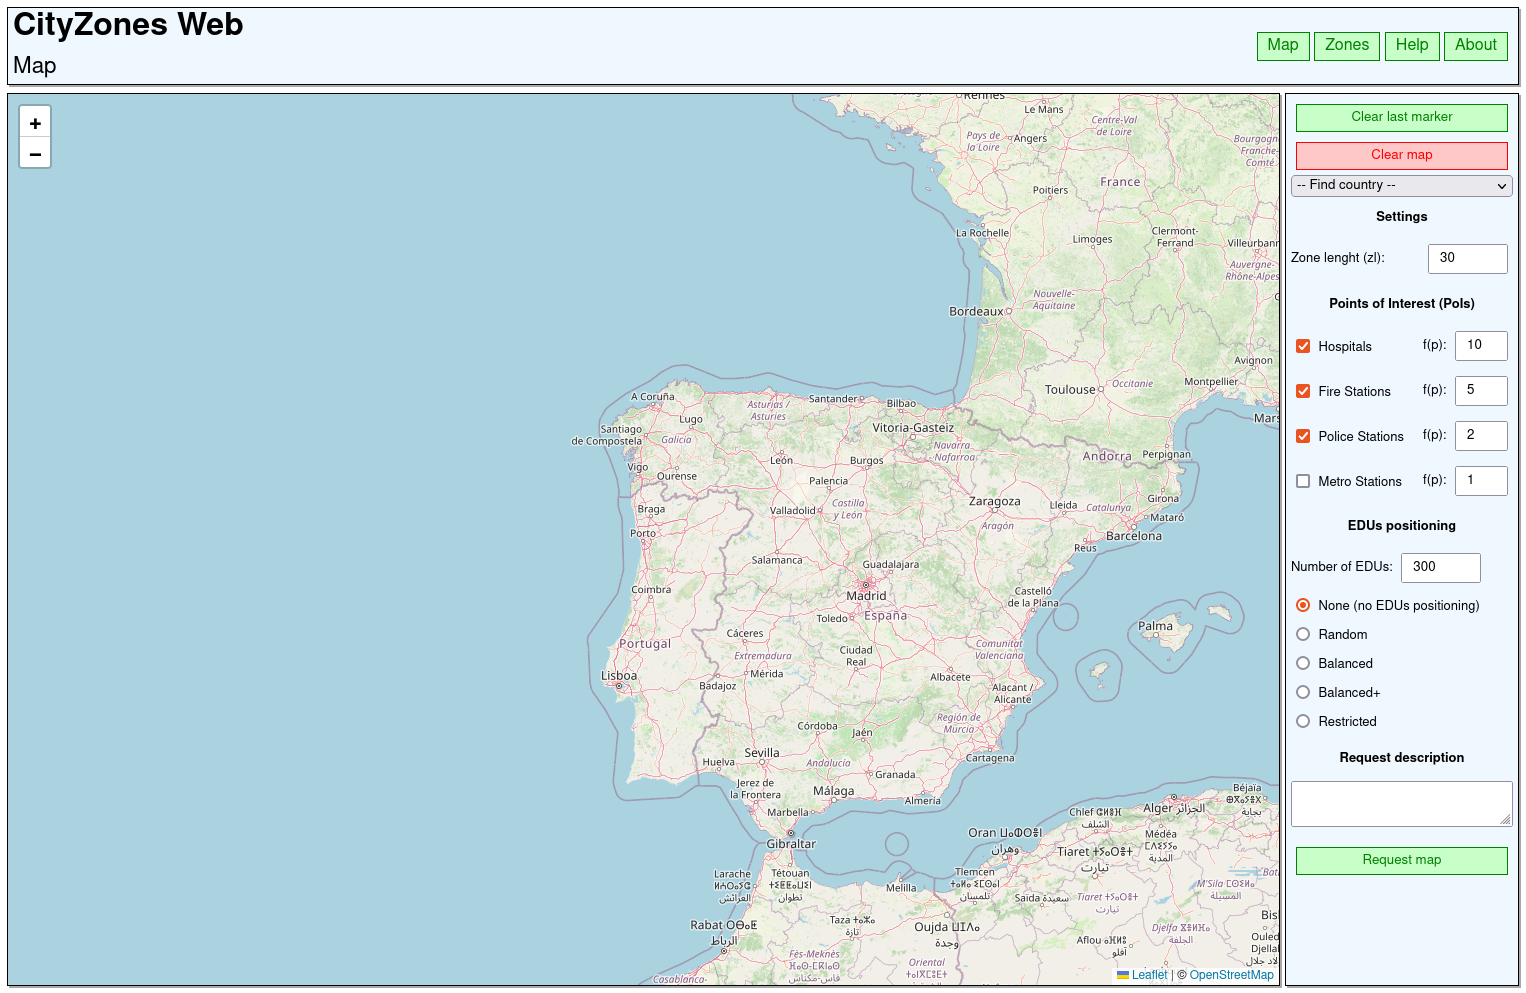
\includegraphics[width=.8\linewidth]{Chapters/3-CityZones/img/cityzones_map.png}
  \caption{A screenshot of the initial page of the CityZones web page.}\label{fig:web_map}
\end{figure}

The toolbar allows the user to clear the visualisation map and start it from scratch, to clear the last mark in case of a mistake, or to upload a GeoJSON file for AoI definition. The most important features are in the settings area of the toolbar, which contains the options for the task processing. The user can select the parameters of the classification: the zone length, which PoIs will be considered and their relevance weight ($f(p)$), the number of EDUs to position, and which positioning algorithm the RiskZones module will use (we implemented four different algorithms). At the bottom of the settings bar there is a input area so the user can write a description of the task for debugging and tracking.

Figure~\ref{fig:web_map_aoi} presents the map view with an user-defined AoI for the city of Porto, Portugal.

\begin{figure}[htb]
  \centering
  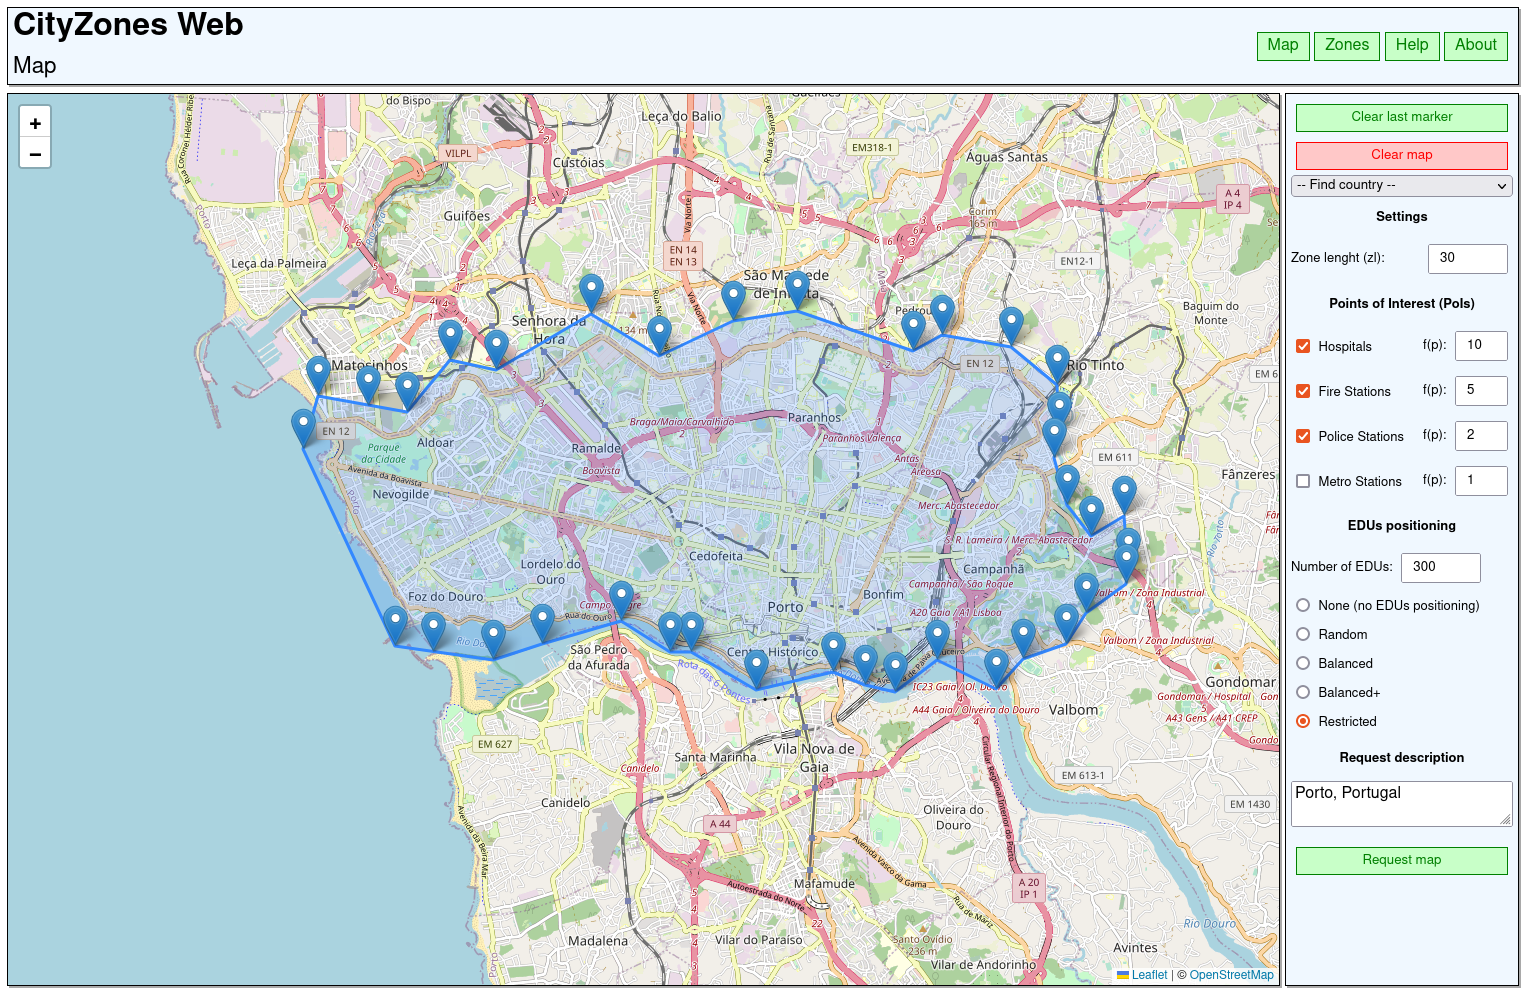
\includegraphics[width=.8\textwidth]{Chapters/3-CityZones/img/cityzones_map_aoi.png}
  \caption{A screenshot presenting a defined AoI for the city of Porto, Portugal.}\label{fig:web_map_aoi}
\end{figure}

After defining an AoI and the configuration of a task, the user can submit it by clicking on ``Request map'' button.  The ``Tasks view'' function in the Client shows all the submitted tasks and their status. New tasks are in the QUEUED state, meaning that the task is ready to be processed, but no Maps-service worker has requested it yet. When a task is assigned and transmitted to a Maps-service, it goes to the PROCESSING state, considering that a single task is assigned to no more than one Maps-service worker.

If a task takes more than one hour to be processed, it is assumed as EXPIRED and returns to the queue of the Application server. This allows the reassignment of a task to any requesting Maps-service worker. Additionally, when the same task is assigned three times in a row, with no computed result, it is assumed as FAILED. This may happen when the configuration is somehow invalid, or when a too large or incorrect AoI polygon is defined.

When a task is finished and the Application server receives the corresponding results, it gets into the DONE state. After that, a user can click the ``Show map'' button in the tasks list to view the resulting classification and EDUs position on map. If needed, the user can also download both the configuration used by the RiskZones module and the result CSV files generated by it using the two links at the task row. The configuration files can be used locally by the user in the RiskZones module and the CSV files can be used in other GIS softwares, including QGIS~\cite{qgis} and Google Earth Engine~\cite{earth}. Also, the list provides a third link that allows the user to repeat the same AoI in another task.

The tasks list in the ``Tasks view'' area displays information about the task. An example of that is presented in Figure~\ref{fig:web_zones}.

\begin{figure}[htb]
  \centering
  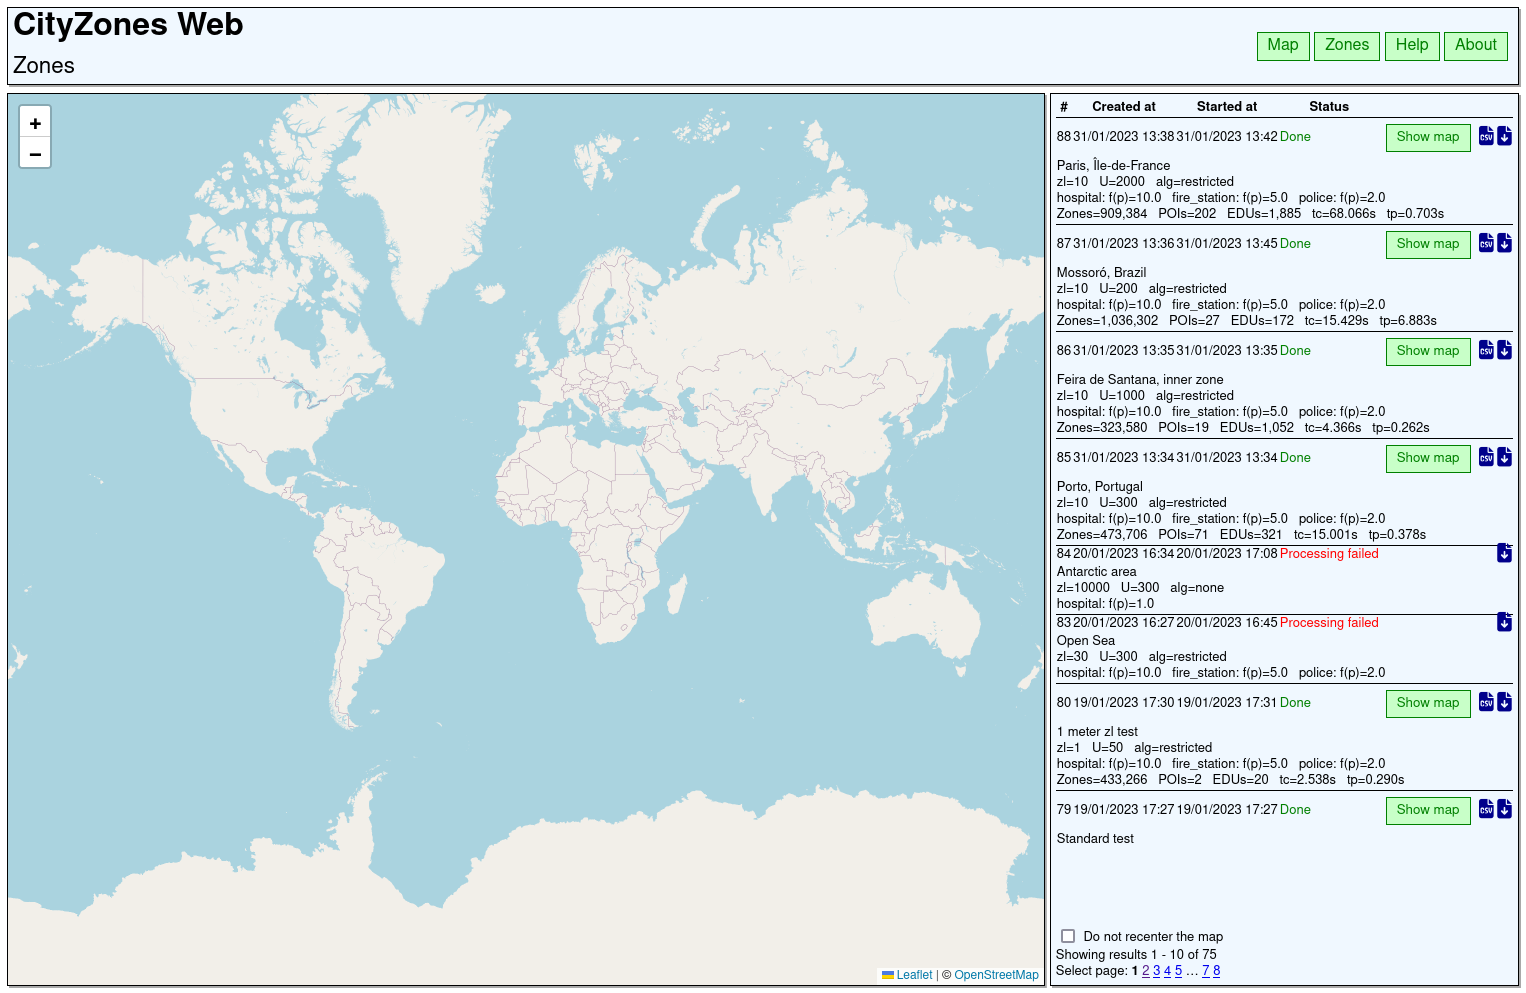
\includegraphics[width=.8\linewidth]{Chapters/3-CityZones/img/cityzones_zones_list.png}
  \caption{A screenshot presenting a list of task with different status.}\label{fig:web_zones}
\end{figure}

After clicking the ``Show map'' button to visualise the results of a classification, a heat-map for the AoI classification is shown, with red being the worst configuration while green is the best. A slider at the bottom of the list allows the user to set the opacity of the heat-map for proper visualisation on the map. Also, a ``Download map image'' button is provided so the user can download a PNG image file of the map shown on the screen. Finally, when properly indicated by the user, the computed map will present the position of the EDUs on the AoI, which are indicated by black dots.

\section{Illustrative example}

\subsection {Risk zones in Berlin}

The presented example in this section is based on the city of Berlin, Germany, which has a total area of 891.82~km$^2$. For that city, any configuration of an AoI is possible, comprising only the area of Berlin or even spreading across multiple adjacent cities. Actually, as an AoI can be any polygon, we can define it by surrounding the Berlin's perimeter, delimiting only this area to define a task, which results in an AoI containing 50 points.

For the initial defined task, the settings in Table~\ref{tab:example_parameters} were considered.

\begin{table}[htbp!]
  \centering
  \begin{tabular}{llp{7.3cm}}
    \hline
    \textbf{Parameter}   & \textbf{Value}      & \textbf{Description} \\
    \hline
    $zl$                 & 30~m                & Size of a squared-sized zone \\
    $U$                  & 2.000               & The total number of EDUs to deploy \\
    $f(hospital)$        & 10                  & Relevance weight of hospitals \\
    $f(fire\_station)$   & 5                   & Relevance weight of fire departments \\
    $f(police\_station)$ & 2                   & Relevance weight of police stations  \\
    $f(metro\_station)$  & 0                   & Relevance weight of metro stations  \\
    Algorithm            & \textit{restricted} & EDUs positioned on streets \\
    \hline
  \end{tabular}
  \caption{Parameters for the initial defined task in these examples.}\label{tab:example_parameters}
\end{table}

After defining the settings, the first task was submitted using the proper button on the CityZones web interface. After being stored by the Application server, it was eventually retrieved by a Maps-service worker, which processed it and returned the final results when concluded. Those results was finally delivered to the Client, being presented as shown in Figure~\ref{fig:berlin_results1}, for a total of 1,199,092 computed zones and 239 PoIs. 

\begin{figure}[!htb]
  \centering
  \subfigure[Results for the initial CityZones classification.]{
    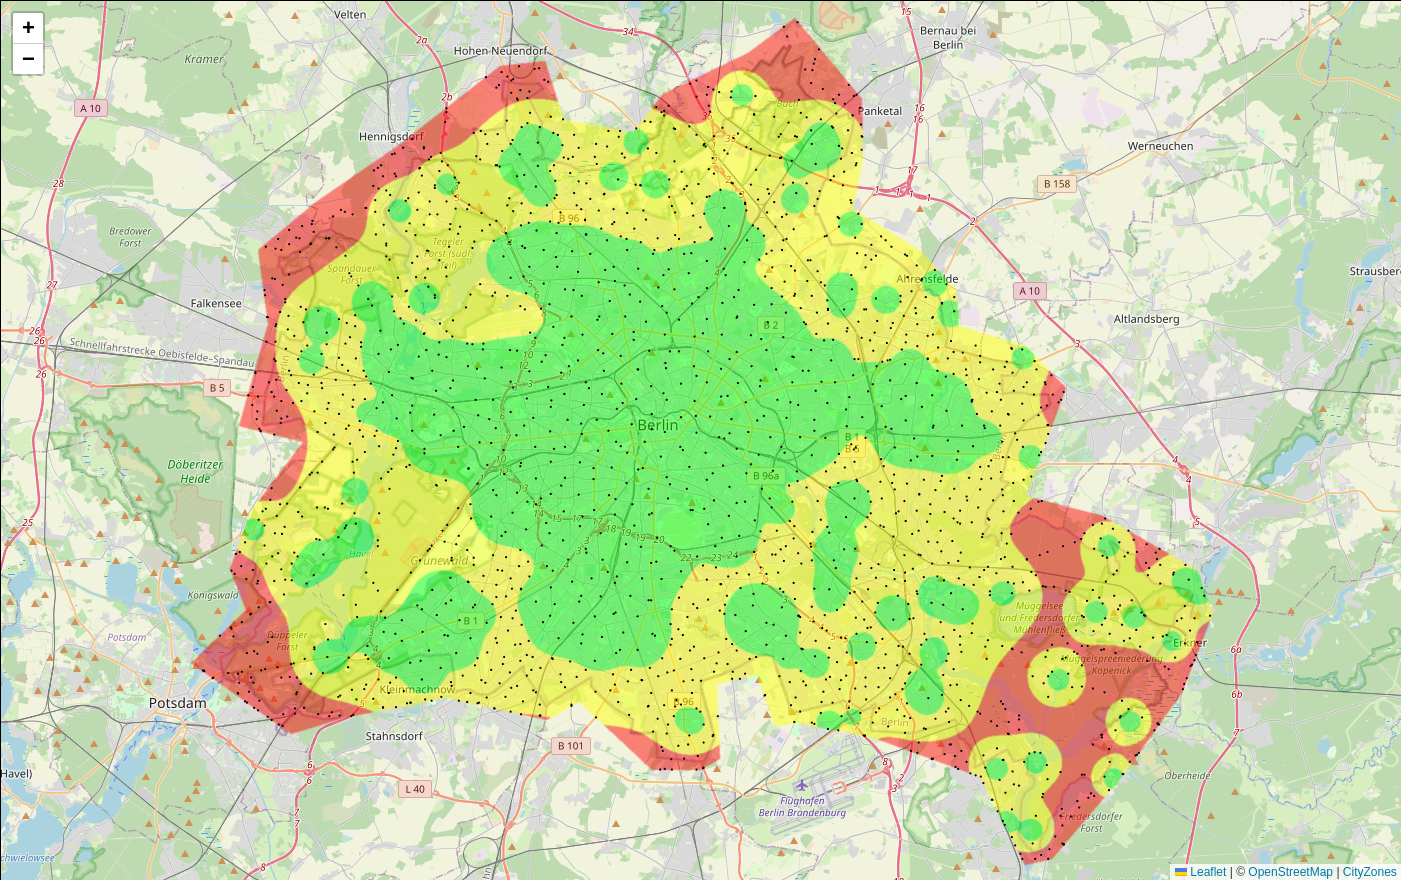
\includegraphics[width=.63\linewidth]{Chapters/3-CityZones/img/berlin/result1.png}\label{fig:berlin_results1}
  }
  \\
  \subfigure[Results for the second task.]{
    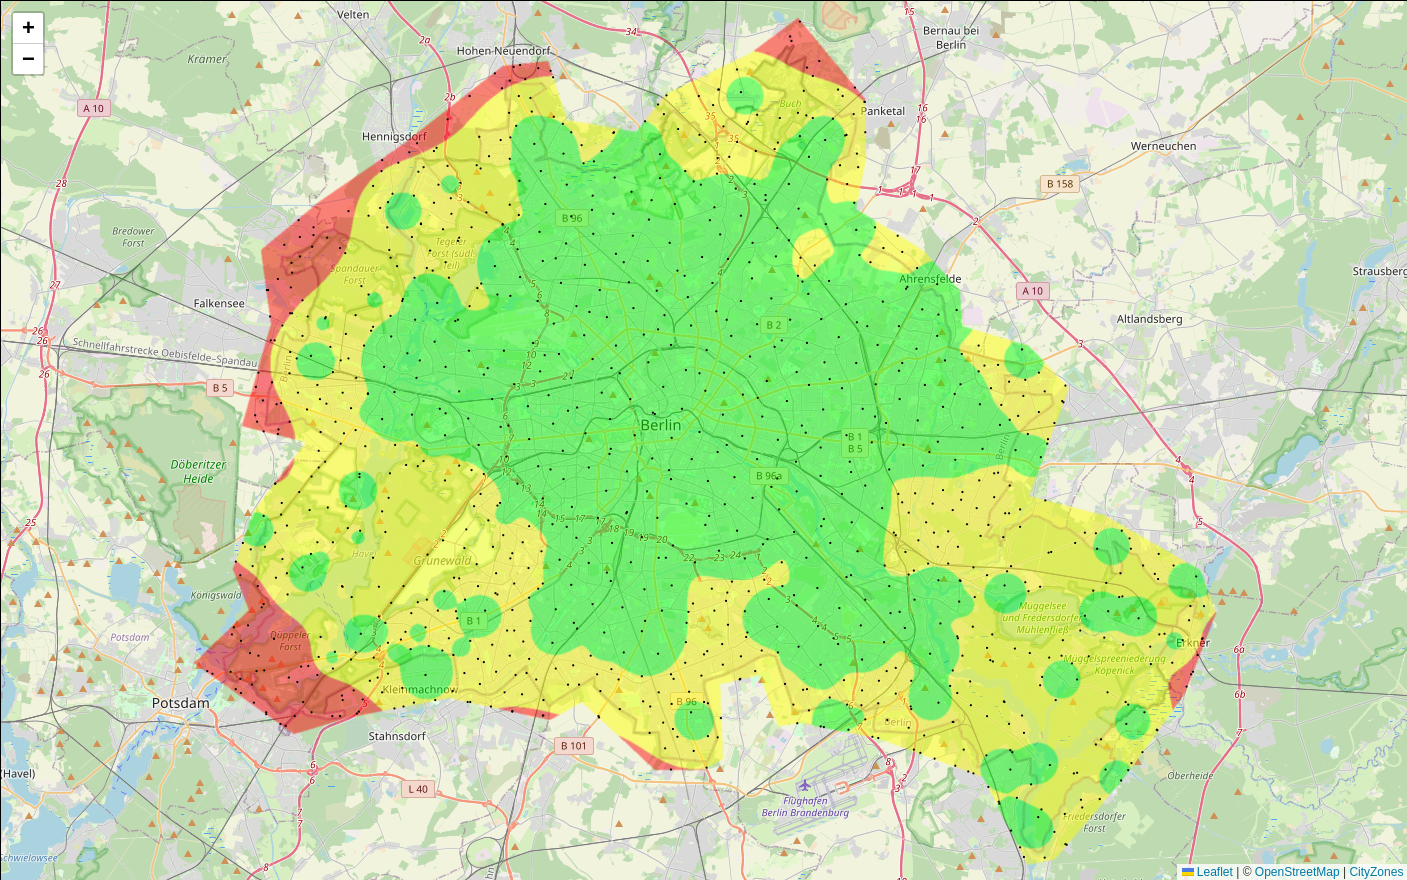
\includegraphics[width=.63\linewidth]{Chapters/3-CityZones/img/berlin/result2.png}\label{fig:berlin_results2}
  }
  \\
  \subfigure[Results for the third task.]{
    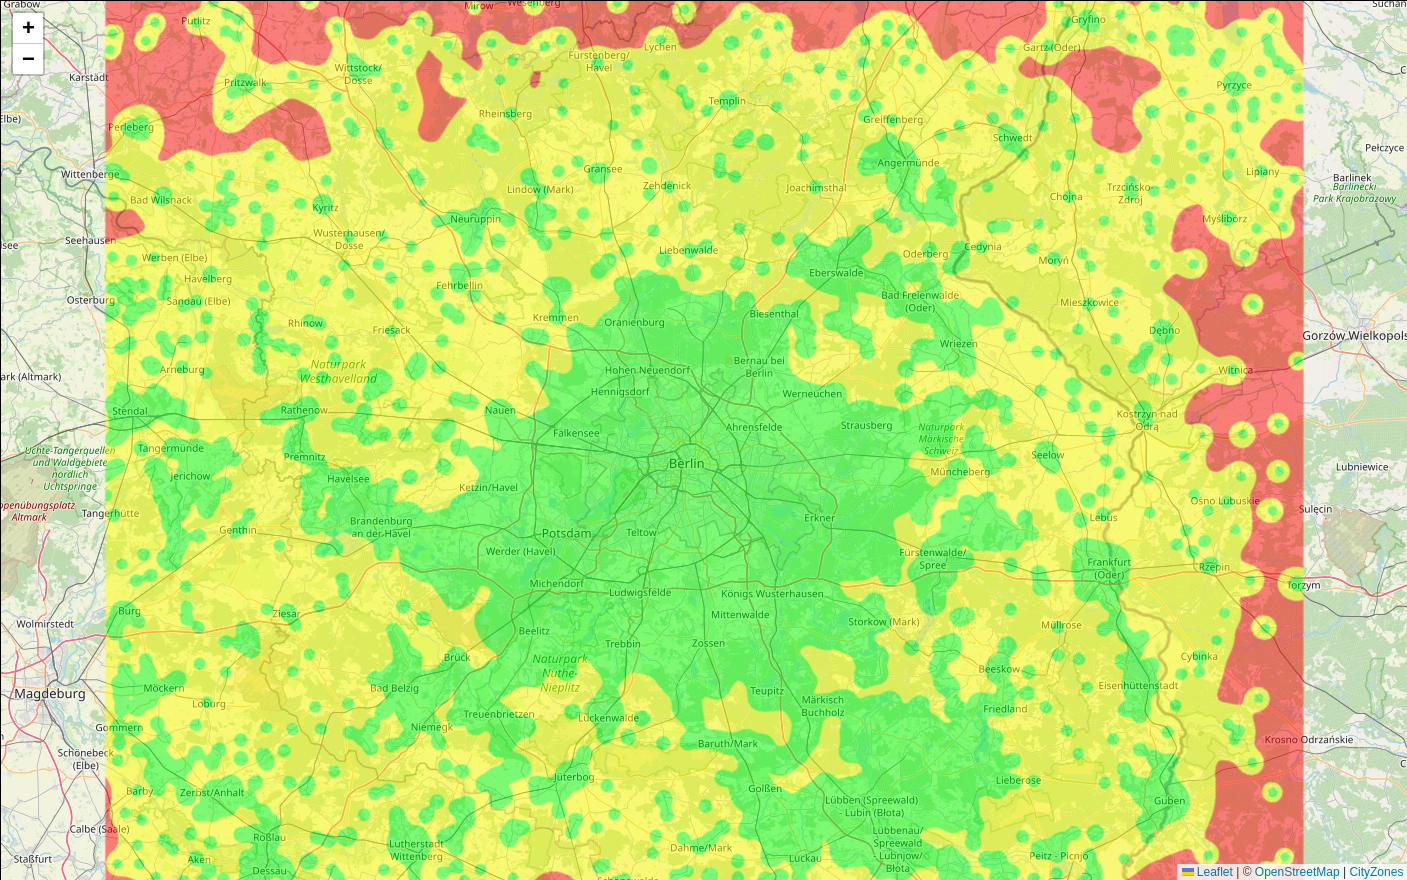
\includegraphics[width=.63\linewidth]{Chapters/3-CityZones/img/berlin/metropolitan_default_noedu.png}\label{fig:berlin_results3}
  }
  \caption{Computed classifications for Berlin. Red areas represent high risk, yellow areas represent medium risk, and green areas represent low risk.}
\end{figure}

The number of zones in an AoI depends not only on its area, but also on the zone length ($zl$). In this scenario, the zone length was 30m. For more detailed results, smaller zones could be used, but more zones would be generated for the same area (higher computational cost). For instance, another test was performed with a zone length of 10m for the same AoI, which resulted in an AoI with 10,797,265 zones. It is possible to set the zone length as lower as 1 meter, but the amount of memory it would need might terminate the RiskZones process due to hardware limits of the running device.

A second test was also conducted for the same AoI. In this test, some parameters were changed: the number of EDUs ($U$ parameter) was reduced by half, while the weight of the PoIs was changed in order to intentionally have a PoI type with a much higher weight than the others, in this case, the fire departments, with results depicted in Figure~\ref{fig:berlin_results2}.

It is noticeable that the heat-map has changed, prioritising the fire station PoIs, thus, zones that were in red in Figure~\ref{fig:berlin_results1} get in yellow or green in Figure~\ref{fig:berlin_results2} if they are near fire stations. This example demonstrates how different results may be produced depending on the settings of the task.

As a third example of using the CityZones tool, a very large AoI was defined surrounding the city of Berlin and taking parts of its metropolitan area, comprising a total area of 35,987.16~km$^2$ and with zones sizing 100m. Moreover, we set $f(hospital)=10$, $f(fire\_station)=5$, $f(police\_station)=2$, and $f(metro\_station)=0$, with $U=0$ (no EDUs positioning was requested). The results for this configuration are presented in Figure~\ref{fig:berlin_results3}, totalling 3,598,716 processed zones for 1,884 PoIs.

The distribution of zones are now different from the other examples because of the change in the AoI. Since the risk levels assignment are relative to the whole area, it is expected that different classifications are obtained with different areas.

%%%%%%%%%%%%%%%%%%
\subsection{Performance evaluation}

The CityZones tool can be implemented in any hardware that supports minimum communication and processing functions, but it is recommended that reasonable processing power is available specially when multiple tasks are requested within a period of time. Currently, the Application server is hosted in a regular cloud-based service as it does not demand much processing power. However, since a Maps-service device will have to process the zones and PoIs for each AoI, also computing the risk zones, it should have reasonable memory and processing resources. An initial Maps-service device was implemented in a computer with an Intel i9 12th generation processor, 64GB DDR5 RAM memory, and 2TB of SSD storage, which is located at the University of Porto. Actually, while the Application server is publicly accessible on the Internet, a Maps-service can operate under any NAT-based network because tasks are requested by it to the Application server, asynchronously. Moreover, as a multi-core processor was selected to be used by the reference Maps-service device, the MultiProcessing Python library is used by the RiskZones module to achieve parallel processing and reduce the overall computation time with the cost of using 100~\% of all CPUs. Regarding the memory usage, the RiskZones module create a list of zones to manage the data of the AoI with each zone consuming 272~bytes, thus, the amount of memory usage depends on how many zones will be instantiated by the module, which is directly related to the area of the AoI and the length of each zone.

Since all the processing is performed in the Maps-service device, the required time for risk classification and EDUs positioning depends on the computer system that is processing the task. Table~\ref{tab:performance} shows some results for tasks processed on the reference Maps-service. 

\begin{table}[htbp]
  \centering
  \begin{tabular}{p{2.3cm}llllll}
    \hline
    \textbf{Region}         & \textbf{AoI points} & \textbf{Zones} & \textbf{PoIs} & \textbf{EDUs} & \textbf{$t_c$ (s)} & \textbf{$t_p$ (s)} \\
    \hline
    Berlin, DE              & 50         & 1,199,092 & 239    & 2,014  & 103.516   & 275.158 \\
    Berlin surroundings     & 4          & 3,598,716 & 1,884  & 0      & 2,324.803 & - \\
    Paris, FR               & 26         & 909,383   & 161    & 2,024  & 53.915    & 144.984 \\
    Porto, PT               & 39         & 473,705   & 60     & 305    & 12.472    & 24.340 \\
    Feira de Santana, BR    & 18         & 355,556   & 19     & 1,002  & 4.059     & 34.061 \\
    \hline
  \end{tabular}
  \caption{Performance of executed tasks, with $t_c$ as the classification time and $t_p$ as the EDUs positioning time.}\label{tab:performance}
\end{table}

Although the final processing time depends on the available hardware resources, the performance of the RiskZones module also depends on the number of zones, PoIs and points that form the AoI polygon. Moreover, regarding the performance of EDUs positioning using the restricted positioning algorithm~\cite{riskzones}, the arrangement of the allowed zones (in this case, the position and form of streets in the AoI), will also influence the time it takes to finish the processing.

It is worth noting that Tiers 1 and 2 do not perform any processing for the classification and positioning steps. Tier 1 only serves as an interface for sending and viewing tasks, while Tier 2 acts as a central data repository, storing and providing task data. Therefore, all performance metrics are measured in Tier 3, where the actual processing takes place.


%%%%%%%%%
\section{Impact}

The CityZones tool may have a significant impact on emergency management in cities. In an initial perspective, it provides stakeholders with an essential tool to identify areas that require urgent attention in case of an emergency. With the risk maps produced by the tool, decision-makers can easily determine the priority of emergency detection in different regions, and plan for mitigation services accordingly. This information is crucial in improving the preparedness of cities for emergencies, which is a critical aspect of public safety. In fact, by identifying the potential risks of different areas in a city, emergency responders can better prepare for potential emergencies and allocate their resources more effectively, potentially leading to faster response times and more efficient use of resources, ultimately saving lives and minimising damage.

The CityZones tool not only helps in understanding the current resilience of cities to emergencies but also extends its impact by identifying potential positions for sensor-based Emergency Detection Units (EDUs). With the efficient deployment of these units, the tool can further improve emergency management systems that operate around the active detection of critical situations by real-time sensing.

Overall, the CityZones tool has great potential for improving the resilience of urban areas in emergency situations, making it a valuable asset for smart city scenarios. The scalability of the tool, enabled by cloud-based servers for processing risk zone computations, makes it capable of handling multiple requests at once. Additionally, the use of data from the constantly updated OpenStreetMap database means that the tool can be used for cities worldwide. Given these advantages, we consider CityZones to be a significant contribution to the field.

%%%%%%%%%
\section{Conclusion}

The computation of risk maps has wide-ranging implications for various applications, including emergency rescuing, urban planning, smart mobility, real estate valuation, public security reinforcement, crisis management, and disaster avoidance. Therefore, having a reliable computational tool to support the computation of such maps can have a significant impact on how these applications are used in practical scenarios, benefiting society as a whole. 

The CityZones tool was implemented as a multi-tier modularized tool with a well-defined programming interface between the modules. This design enables the inclusion of new modules to support additional services. For instance, the AoI definitions and general maps handling can be completely reused by new services, which is one of the design requirements of the tool.

As future works, the CityZones tool will be extended to incorporate new EDUs positioning algorithms based on research works in the literature. Additionally, other types of PoIs will be also considered, taking for example major road junctions and real-time positions of response vehicles as new mitigation-related input parameters.

%%%%%%%%%
% \section*{Acknowledgement}

This work was supported by national funds through the FCT/MCTES (PIDDAC), under the project EXPL/EEI-COM/1089/2021. It is also supported by INEGI-LAETA (FCT project UIDB/50022/2020). Finally, this work was financed in part by the Coordenação de Aperfeiçoamento de Pessoal de Nível Superior - Brasil (CAPES) - Finance Code 001.

\printbibliography[heading=subbibliography]

\end{refsection}

    \selectlanguage{portuguese}

    %%----------------------------------------------------------------------------
    %% Inclui anexos
    %%----------------------------------------------------------------------------
    % Comente qualquer linha que não queira inserir
    \begin{thesisappendices}
        %\chapter{Anexo I}
\label{anex1}
\begin{center}
    \textbf{Aqui pode ser um Título do seu Anexo}
\end{center}

Texto do Anexo.

        % Caso precise de mais anexos, basta criar novos arquivos e acrescentá-los
        % aqui seguindo o modelo acima
    \end{thesisappendices}

    %%----------------------------------------------------------------------------
    %% Configurar as referencias bibliográficas
    %%----------------------------------------------------------------------------
    % \addcontentsline{toc}{chapter}{Referências}
    %\bibliographystyle{abntex2}
    %\bibliography{refs}

    %\bibliographystyle{unsrt}
    %\bibliographystyle{abnt}
    % \bibliography{References/refs_tese}
    
    %%----------------------------------------------------------------------------
    %% Finalização
    %%----------------------------------------------------------------------------
    %==========================================================
%        Document: PPGM-UEFS
%        File....: UltimaFolha.TEX
%        Author..: Gilney Zebende
%        Date....: 24 de abril de 2018
%==========================================================
\begin{ultimafolha}

\vspace*{\fill}

\begin{flushleft}
{\it \thetitle} \\
\ \\
\theauthor \\
\ \\
\ppgmcidade, \ppgmmes\space de \ppgmano.
\end{flushleft}
\end{ultimafolha}

\end{document}

%%%-------------------------------------------------------------------------------
%%% Aqui finalizamos a formatação. Faça um bom trabalho.
%%%-------------------------------------------------------------------------------
